% Hyperparameter optimization survey and implementation guide.
% Build: pdflatex main && bibtex main && pdflatex main && pdflatex main
% Fonts: mathptmx + helvet (newtxtext/sourcesanspro are not installed on this machine).
\documentclass[11pt]{report}

\usepackage[margin=1.1in]{geometry}
\usepackage{mathptmx}
\usepackage[scaled=0.92]{helvet}
\usepackage{microtype}
\usepackage{amsmath,amssymb,bm}
\usepackage{booktabs,longtable,array,tabularx}
\usepackage{enumitem}
\usepackage[round]{natbib}
\usepackage{xcolor}
\usepackage{framed}
\usepackage{caption}
\usepackage{url}
\usepackage{tikz}
\usetikzlibrary{positioning,arrows.meta,calc,decorations.pathreplacing}
\usepackage[colorlinks=true,linkcolor=blue!50!black,citecolor=blue!50!black,urlcolor=blue!60!black]{hyperref}

\setlength{\emergencystretch}{2em}
\bibliographystyle{plainnat}

% Decision boxes: the operational layer for readers deciding what to build.
% A thick left rule marks them; they restate section verdicts in plain terms
% and are skippable by readers following the teaching layer.
\newenvironment{decisions}{%
  \def\FrameCommand{{\color{blue!50!black}\vrule width 2.5pt}\hspace{8pt}}%
  \MakeFramed{\advance\hsize-\width\FrameRestore}\small}%
{\endMakeFramed}

\newcommand{\config}{\bm{\lambda}}
\newcommand{\cspace}{\Lambda}
\newcommand{\E}{\mathbb{E}}
\newcommand{\R}{\mathbb{R}}
\newcommand{\N}{\mathcal{N}}
\newcommand{\gp}{\mathcal{GP}}

\title{Tuning the machines that tune themselves:\\
a survey of hyperparameter optimization\\
and a plan for building our own tuner}
\author{Internal research note, prepared for the workspace projects\\
(reinforcement learning, Hamiltonian networks, neural-transport samplers,\\
multi-objective models)}
\date{August 24, 2026}

\begin{document}
\maketitle

\begin{abstract}
We are planning a shared hyperparameter-tuning system for the training
workloads in our workspace: reinforcement learning through RLlib,
Hamiltonian neural networks, neural-transport samplers, and
multi-objective models. This document surveys the tuning literature
through August 2026 at a level meant to teach, with the load-bearing
mechanisms derived in place and illustrated on one running example
rather than quoted from their papers, audits the open-source tooling
library by library against primary sources, and turns both into an
implementation plan.

The architectural conclusion is to keep Ray Tune
as the execution layer (its distributed trials, checkpointing, and
population-based training remain the strongest available, and we already
operate Ray) while owning the search layer ourselves, since Tune's
algorithm side has been in maintenance while method development moved to
Optuna, BoTorch, and the AutoML groups' libraries.

The algorithmic
conclusion is a tiered roadmap: asynchronous successive halving plus a
carefully configured Bayesian optimizer as the spine; noise-aware
multi-objective acquisition with multi-objective early stopping, expert
priors, cost-aware search, and the PB2-to-BG-PBT population line for
reinforcement learning as the differentiators; freeze-thaw scheduling
with a pre-trained learning-curve surrogate as the frontier bet. Each
recommendation is tied to the controlled evidence that supports it, and
a validation suite is specified before any of it is built.

\end{abstract}

\setcounter{tocdepth}{1}
\tableofcontents
\clearpage

\part{The problem}
\chapter{Introduction}
\label{sec:intro}

This document answers two questions we posed ourselves while planning a
shared tuning system for the projects in our workspace: whether Ray Tune
is the right architecture to build on, given that RLlib already runs our
reinforcement-learning work, and which algorithms such a system should
implement to serve very different customers, from reinforcement-learning
agents through Hamiltonian neural networks and neural-transport samplers to
multi-objective models in finance. Both questions turn out to have
reasonably confident answers once the literature is laid out, and laying
it out carefully is most of the document: our local paper collection
thins out around 2023, and several things a 2023 reader would recommend
are no longer what a 2026 reader should build.

The short answers, defended over the following chapters; the method
names that follow are only names for now, each taught from zero in its
chapter, so read this section as a map to return to rather than an
argument to absorb. Ray Tune: yes,
as the execution layer, and deliberately not as the source of search
algorithms. Tune's distributed trial execution, checkpoint machinery, and
population-based training support remain the strongest in open source and
compose naturally with RLlib, but its own algorithm layer has been in
maintenance for roughly two years while the method frontier moved into
other projects (Chapters~\ref{sec:libraries}
and~\ref{sec:architecture}).

The algorithms: a spine of asynchronous successive halving plus a
well-configured Bayesian optimizer covers the routine work at low cost;
the differentiators worth building are noise-aware multi-objective
acquisition with a multi-objective early-stopping scheduler, expert
priors, cost-aware acquisition, and a population line for reinforcement
learning. The method names that follow are only names for now, each
taught from zero in its chapter: qLogNEHVI with MO-ASHA
(Chapters~\ref{sec:moo}), priors in the PriorBand style
(Chapter~\ref{sec:transfer}), and the population line as PB2 extended to
mixed spaces and then BG-PBT, the method we were specifically asked to
assess (Chapter~\ref{sec:population}). Freeze-thaw scheduling with a
pre-trained learning-curve surrogate is the one frontier bet we recommend
(Chapter~\ref{sec:multifidelity}), and Chapter~\ref{sec:roadmap} puts
the whole list in build order with the evidence attached to each item.

The document is written to teach as well as to conclude, because the
people extending this system next year will need the reasoning, not just
the verdicts, and a verdict whose derivation you cannot reconstruct is
one you cannot safely modify. Three habits follow, and knowing them up
front makes the document easier to read.

First, one running example
carries the whole text: tuning PPO on a Brax locomotion task, in the
fifteen-dimensional search space introduced in
Section~\ref{sec:running}, with a Hamiltonian network as the second
thread wherever several objectives compete. When a formula arrives, its
symbols are read against that example before anything is done with
them.

Second, every load-bearing equation is derived or unpacked in
place rather than quoted: the Gaussian-process posterior, expected
improvement and the floating-point failure that motivates its modern
replacement, the tree-structured Parzen estimator's ratio rule, the
budget arithmetic of successive halving, the geometry that breaks
weighted-sum scalarization.

Third, the figures are schematic drawings
of mechanisms, not plots of measured data, and their captions say what
each one is supposed to show; when a number matters, it is computed in
the text where the reader can check it.

The document also carries a decision layer, kept visually separate from
the teaching so that neither gets in the other's way. Each method
chapter ends in a boxed \emph{Decisions from this chapter} marked by a
thick left rule: plain-language verdicts, include or exclude, with the
cost to build, the evidence behind the call, and the comparison against
the alternatives, written to be judged without opening any cited paper.

The box is earned rather than asserted: each method chapter closes by
first teaching the experiments its verdict rests on, their designs,
arenas, and sponsors, so the evidence can be judged rather than taken
on citation, and then arguing the verdict from several independent
angles, ending with the criterion that would overturn it in our own
validation suite.

Table~\ref{tab:decisions} in Chapter~\ref{sec:roadmap} collects every
verdict on one page. A glossary at the end defines every term of art in
plain language. And because several of our readers come from economics
and statistics rather than machine learning, the text flags the bridges
where they exist: the Gaussian process is kriging, expected improvement
is an option value, the Pareto front (the set of configurations
undominated in objective space) is the welfare-theoretic one.

Chapter~\ref{sec:problem} pins down the problem, fixes the running
example, and maps the four ways our workloads bend the textbook
formulation. Chapters~\ref{sec:modelfree} through~\ref{sec:transfer}
build up the method families in increasing order of structure: searching
without a model, modeling the objective, exploiting partial evaluations,
tuning while training, handling several objectives, and importing
knowledge from priors, past studies, and scale. Each chapter opens with
the failure of the previous chapter's best answer, which is not a
storytelling flourish: it is the actual dependency structure of the
field, and it is why the chapters are in this order.

Chapter~\ref{sec:workloads} turns back to our four workload families and
says what to do for each. Chapter~\ref{sec:libraries} audits the
open-source field library by library, with maintenance status checked
against primary sources on August 22, 2026, and re-verified on
August 23. The closing part turns the verdicts into a concrete product
proposal: Chapter~\ref{sec:product} states what we ship and walks a
first study through it, Chapter~\ref{sec:architecture} gives the
architectural design, Chapter~\ref{sec:contracts} pins the interfaces
and data schemas, Chapter~\ref{sec:validation} specifies the test
suite, and Chapter~\ref{sec:roadmap} the build plan and the bill.

A reader who wants
only decisions can read Chapter~\ref{sec:problem}, the decision boxes
at the ends of Chapters~\ref{sec:modelfree}
through~\ref{sec:workloads}, and then Chapters~\ref{sec:libraries},
\ref{sec:architecture}, and~\ref{sec:roadmap} with
Table~\ref{tab:decisions}; a reader implementing a searcher should
read the method chapters in order, since each one leans on the
machinery of its predecessors.

A note on sourcing. Claims about specific methods are tied to the papers
that introduced or tested them, and the load-bearing ones (BG-PBT, the
RL tuning study of Eimer, Lindauer, and Raileanu, and the current
defaults of the major libraries) were checked against the primary texts
and pages rather than summaries; a companion file records, for every
source, what was inspected and at what depth. The derivations added for
teaching (Gaussian conditioning, the expected-improvement closed form
and its underflow arithmetic, the successive-halving budget count, the
hypervolume and scalarization geometry) are elementary and stand on
their own; they explain the cited results rather than extend them.
Where a comparison rests on one paper's experiments we say so, and
where the honest answer is that two methods are indistinguishable on
current evidence, we say that too, in preference to manufacturing a
ranking.

\chapter{The problem we are actually trying to solve}
\label{sec:problem}

Every project in our workspace trains something: a reinforcement-learning
(RL) agent through RLlib (Ray's RL library), a Hamiltonian
neural network on trajectory data (a network whose architecture builds in
energy conservation), a normalizing flow that preconditions a sampler (a
neural map that reshapes a hard posterior into an easier one), a
forecasting model with several competing losses. Each of these is taught
properly where it matters (Chapter~\ref{sec:workloads} devotes a section
to each); for now they are simply the customers. Each of these training procedures exposes ten to twenty
knobs, and the knobs come in four kinds. The kinds are worth meeting one
at a time, because every method in this document has to handle all four,
and more than one otherwise-good method stumbles on exactly one of them.

A \emph{continuous} knob takes any value in an interval. The learning
rate is the canonical case: $3 \times 10^{-4}$ is a legal setting, so is
$2.9 \times 10^{-4}$, and so is everything between them. Entropy
coefficients and integrator step sizes are the same kind. Continuous
knobs are the friendliest kind, because ``nearby'' means what it seems
to mean: settings close together usually behave similarly, and every
model-based method in this document leans on that.

An \emph{ordinal} knob is an integer with a natural order. Batch size
runs 128, 256, 512; network width and the number of integrator steps
inside a sampler are the same kind. The order carries real information, since 256 genuinely
sits between 128 and 512 and performance usually moves through it on
the way from one to the other, but the grid is coarse, and treating
the values as just another continuum papers over the coarseness. How
much that ordering is worth respecting returns as a concrete design
choice in Chapter~\ref{sec:bayesian}.

A \emph{categorical} knob is a choice among labels with no ``between''
at all. There is no activation function halfway from $\tanh$ to ReLU,
and no gradual path between using spectral normalization (a training
stabilizer we will meet again in the running example) and not using
it. Methods built on continuity must do something special here, and
what they do (overlap kernels, per-category bandits) occupies real
space in Chapters~\ref{sec:bayesian} and~\ref{sec:population}.

A \emph{conditional} knob exists only when another knob takes a
particular value. Learning-rate annealing is the standing instance: if
annealing is switched off, the final learning-rate multiplier is not
merely irrelevant, it is undefined, and a tuner that keeps proposing
values for it is spending budget on configurations that do not differ.
(Off-policy algorithms supply the same structure elsewhere in our
workloads: the temperature of a soft target update is undefined when
hard updates are selected.)
Conditional structure is why realistic search spaces are trees rather
than boxes, and it decides real verdicts later; it is much of the case
for one of Chapter~\ref{sec:bayesian}'s searchers.

Choosing these values well is routinely worth more than
the next clever idea, and choosing them badly can make a sound method look
broken. \citet{eimer2023hyperparameters} swept eleven hyperparameters of
PPO, the same reinforcement-learning algorithm our running example will
tune below, across standard environments and found that almost every one of them had a
large effect on final return in at least one environment, including knobs that
most papers never tune, such as the clipping range. The same study found that
the worst value of a swept hyperparameter landed within one standard deviation
of the best value in only 7 of 126 sweeps. Tuning is not optional in our line
of work; the only question is how much compute and attention it consumes.

\section{A running example, and the loop every method lives in}
\label{sec:running}

Abstract definitions slide off the mind unless they have something to stick
to, so we fix a concrete case now and return to it in every section. Our
running example is the one our own cluster runs most often: tuning PPO,
the workhorse reinforcement-learning algorithm of our RLlib stack, as it
learns a locomotion task in Brax, a suite of fast physics-simulated
environments.

Since PPO's knobs will follow us through the whole document, one
plain-language pass through the algorithm is worth its space; nothing
deeper than this pass is ever assumed. The agent holds two neural
networks. The \emph{policy} maps what the agent observes to a
distribution over actions; the \emph{value network} predicts how much
reward is still to come from a given situation. Training alternates two
activities: the agent acts in the simulated environment for a while,
collecting observations, actions, and rewards, and then the optimizer
takes gradient steps that make the actions which worked out better than
the value network expected (the \emph{advantage}) more probable, with a
clip that keeps the updated policy close to the policy that collected
the data. The name PPO, proximal policy optimization, is a description:
optimize the policy, but stay proximal. A trained agent's score, its
\emph{return}, is the total reward it accumulates over an episode of
play.

The full search space, taken from the experiments behind BG-PBT, the
population-based method Chapter~\ref{sec:population} examines in
detail, has fifteen
dimensions: nine training hyperparameters (learning rate, discount, entropy
coefficient, unroll length, reward scaling, batch size, update epochs,
the generalized-advantage-estimation parameter GAE
$\lambda$, clipping $\epsilon$) and six architecture parameters (width,
depth, and a spectral-normalization flag, separately for the policy and
value networks) \citep{wan2022bgpbt}.

\subsection{Reading the fifteen knobs}

Fifteen numbers is a lot to hold, so read them in groups, by what each
group controls. The aim is not to memorize the list but to see that
each entry is a lever a practitioner can explain, not a mystery
constant.

Three knobs govern the size of an update. The learning rate scales how
far every gradient step moves the network, and it is the most
notorious hyperparameter in deep learning for a reason: too large
diverges, too small never arrives, and the usable range spans decades.
PPO's clipping $\epsilon$ bounds how far one update may move the
\emph{policy} away from the policy that collected the current data, a
trust leash rather than a step size. Reward scaling sets the units of
the training signal itself, and every gradient inherits those units.

Two knobs decide what the future is worth. The discount $\gamma$
weights a reward $t$ steps ahead by $\gamma^{t}$, so it is exactly a
time-preference parameter, and the conventional $\gamma = 0.99$ gives
an effective horizon of about $1/(1-\gamma) = 100$ steps. GAE's
$\lambda$ (generalized advantage estimation) sets how far into the
observed future the advantage estimate
looks, trading the bias of short lookaheads against the variance of
long ones.

One knob buys experimentation. The entropy coefficient pays the policy
a bonus for staying random, so that it keeps trying actions it would
otherwise have abandoned. Too little and the agent commits early to a
mediocre habit; too much and it never commits at all.

Three knobs meter the data per update: the unroll length (how many
environment steps are collected before an update), the batch size (how
many of those steps each gradient estimate averages over), and the
number of update epochs (how many passes the optimizer makes over the
same collected data before discarding it).

The remaining six are the architecture: width and depth for the policy
network and again for the value network, capacity in four integers,
plus a spectral-normalization flag for each, a stabilizer and our
standing example of a categorical knob.

None of these levers acts alone. The size of a stable gradient step
depends on how much data estimated it, so batch size and learning rate
tend to move together; a longer unroll changes what $\gamma$ and
$\lambda$ can see; extra capacity changes how much restraining the
entropy bonus and the clip must do. This coupling is why turning one
knob at a time misleads, and why methods that model the joint surface
(Chapter~\ref{sec:bayesian}) earn their complexity. Whenever a figure
needs a space we can draw, we will slice out the two knobs everyone
recognizes: the learning rate, searched on a log scale from $10^{-5}$
to $10^{-2}$, and the entropy coefficient.

\subsection{Expensive, noisy, and without gradients}

One evaluation of one configuration means training an agent for up to
150 million environment steps, hours of wall-clock on several
accelerators. Everything else in this document is downstream of that
number: a hundred-trial study is hundreds of GPU-hours, a line item
someone has to defend, and Section~\ref{sec:costmodel} prices it out.

The resulting score is noisy. Each training run reports the mean
evaluated return over a handful of episodes, and two agents differing only in
random seed can land far apart. When the formal statement below takes
an expectation over seeds, this spread is what the expectation is
pricing.

And the score arrives without gradients in the knobs. Backpropagation
supplies derivatives of the loss with respect to the network's
weights, not with respect to the batch size that fed it or the
discount that shaped its targets; between $\config$ and the final
return stands an entire non-differentiable training procedure. Nothing
like gradient descent is available in the space we are actually
searching.

Expensive, noisy, and gradient-free: those three properties are the
whole reason this document exists.

A second, smaller case will carry the multi-objective thread: a Hamiltonian
neural network from our physics projects, where one training run is minutes
rather than hours, and where nobody can say in advance how many units of long-rollout
energy drift one unit of short-horizon prediction error is worth. We will
meet it properly in Chapters~\ref{sec:moo} and~\ref{sec:workloads}.

\subsection{The loop, and the words for its parts}

Every method in this document, from grid search to the most elaborate
population scheme, is an instance of one loop, and it is worth drawing once
so that later chapters can point at its parts
(Figure~\ref{fig:loop}). A \emph{tuner} holds two responsibilities that we
will keep separate throughout, because the literature develops them
separately and our own design (Chapter~\ref{sec:architecture}) implements
them behind separate interfaces. The \emph{searcher} decides which
configuration to try next. The \emph{scheduler} decides how long each trial
runs, which trials to stop early, and which paused trials to resume. The
executor trains the model and streams back intermediate scores; everything
observed lands in a store that the tuner (and, later, other studies) can
consult. Grid search is this loop with a trivial searcher and no scheduler;
Bayesian optimization upgrades the searcher
(Chapter~\ref{sec:bayesian}); successive halving upgrades the scheduler
(Chapter~\ref{sec:multifidelity}); population-based training entangles the
two on purpose (Chapter~\ref{sec:population}).

\begin{figure}[t]
\centering
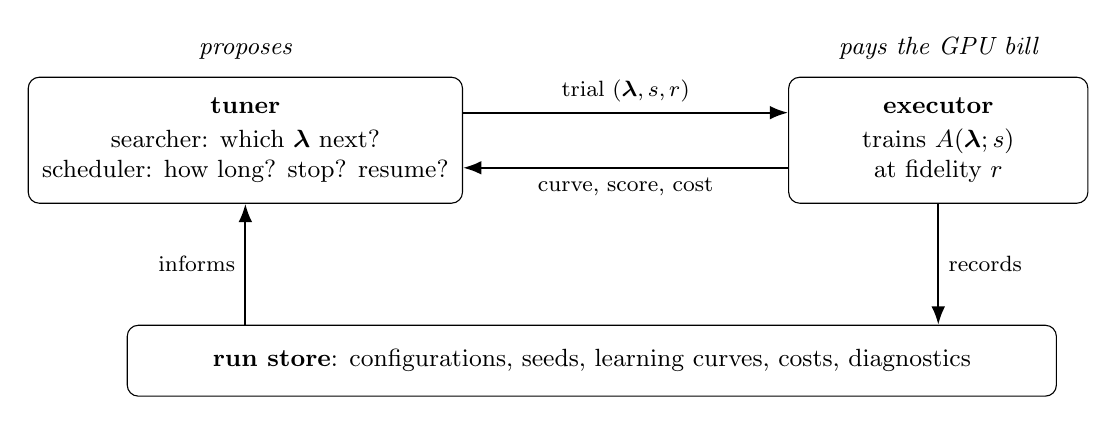
\begin{tikzpicture}[
  box/.style={draw, rounded corners, align=center, inner sep=5pt, font=\small},
  arr/.style={-{Latex}, thick}]
\node[box, minimum width=46mm, minimum height=16mm] (tuner) at (0,0)
  {\textbf{tuner}\\[1pt] searcher: which $\config$ next?\\ scheduler: how long? stop? resume?};
\node[box, minimum width=38mm, minimum height=16mm] (exec) at (8.8,0)
  {\textbf{executor}\\[1pt] trains $A(\config; s)$\\ at fidelity $r$};
\draw[arr] ([yshift=3.5mm]tuner.east) -- node[above, font=\footnotesize] {trial $(\config, s, r)$} ([yshift=3.5mm]exec.west);
\draw[arr] ([yshift=-3.5mm]exec.west) -- node[below, font=\footnotesize] {curve, score, cost} ([yshift=-3.5mm]tuner.east);
\node[box, minimum width=118mm, minimum height=9mm] (store) at (4.4,-2.8)
  {\textbf{run store}: configurations, seeds, learning curves, costs, diagnostics};
\draw[arr] (exec.south) -- node[right, font=\footnotesize] {records} (exec.south |- store.north);
\draw[arr] (store.north -| tuner.south) -- node[left, font=\footnotesize] {informs} (tuner.south);
\node[font=\small\itshape, above=1mm of tuner.north] {proposes};
\node[font=\small\itshape, above=1mm of exec.north] {pays the GPU bill};
\end{tikzpicture}
\caption{The loop every tuning method instantiates. The searcher and the
scheduler are separate decisions: one picks configurations, the other
allocates training budget across them. Everything observed flows into a
store, which is what later lets a new study start smarter than its
predecessor (Chapter~\ref{sec:transfer}).}
\label{fig:loop}
\end{figure}

Three words from the figure recur on nearly every page, so we fix them now.
A \emph{trial} is a single training run with a fixed configuration (and, we
will insist later, a recorded seed). The \emph{incumbent} is the best
configuration found so far. The \emph{fidelity} of a partial evaluation is
its resource level: epochs trained, environment steps consumed, chain length
run. In the running example, a full-fidelity trial is 150 million steps; a
one-tenth-fidelity trial of the same configuration costs one tenth of the
GPU bill and tells us something, but not everything, about the full run.

To see the loop turn once, walk a young study through it. The searcher,
knowing nothing yet, proposes a first configuration: learning rate
$3 \times 10^{-4}$, width 256, annealing off. The scheduler grants
it a tenth of full fidelity, 15 million steps. The executor trains,
streaming back a learning curve, and the store records the
configuration, the seed, the curve, and the bill. At the next decision
point the scheduler looks at that curve and either buys the trial more
steps or stops payment, and the searcher, now holding one completed
record rather than none, proposes a second configuration a little less
blindly. Every chapter that follows upgrades one arrow of
Figure~\ref{fig:loop} and leaves the rest of the loop alone.

\section{The formal problem, and where it bends}
\label{sec:formal}

The textbook formulation is simple, and we will need it on the page because
every method chapter refines some part of it. A training algorithm $A$ maps a
configuration $\config \in \cspace$ and a random seed $s$ to a trained model,
and a cost function $c$ scores that model on held-out data, so we want
\begin{equation}
\config^{\star} \in \arg\min_{\config \in \cspace}
\; \E_{s}\!\left[ c\!\left( A(\config; s) \right) \right],
\label{eq:hpo}
\end{equation}
where the expectation runs over seeds (and, when relevant, over draws of the
training data or of environment instances). Read the pieces against the
running example: $\cspace$ is the fifteen-dimensional product of intervals
(learning rate), integer ranges (width, batch size), and finite sets (the
spectral-normalization flag), sometimes with conditional branches; $A$ is
the machine-learning training loop as a whole, here PPO and everything
around it; $c$ is the negative of the evaluated return; the expectation
over $s$ is the part beginners drop and RL practitioners regret dropping.
Each evaluation of the objective means training a model, so evaluations are
expensive, noisy, and yield no gradients with respect to $\config$. This is
black-box optimization under noise, and Chapter~\ref{sec:bayesian} describes
the machinery built for exactly this setting.

The expectation in \eqref{eq:hpo} deserves one concrete reading before
it starts doing work. Suppose, schematically, that configuration A
trains to evaluated returns of 900 and 300 on two seeds, while
configuration B trains to 640 and 660. A leaderboard that remembers
best single runs crowns A, whose 900 is the best number anyone has
seen. The expectation averages instead, 600 against 650, advantage B,
and that is the right verdict for anyone who must ship one
configuration and then live with whatever seed the production run
draws. Optimizing the average of a noisy objective and optimizing its
luckiest observed value are different problems, and \eqref{eq:hpo}
commits us, deliberately, to the first.

Formulation~\eqref{eq:hpo} bends in four places for our workloads, and each
bend picks out a branch of the literature. The four bends are worth reading
slowly: they are the map of Chapters~\ref{sec:modelfree}
through~\ref{sec:transfer}, and each one will reappear as the opening
problem of its chapter.

\subsection{Bend one: the seed is part of the problem}

The expectation over seeds is not a nuisance term; in reinforcement
learning it is often the dominant source of variation.
\citet{eimer2023hyperparameters} observed single seeds crashing while sibling
seeds of the same configuration finished well, and found that a configuration
selected on one seed can sit far below average on others. Concretely: if we
tune the running example on seed 1 and the winning configuration happened to
draw a lucky initialization, we have optimized for the luck, not the
configuration, and the ``win'' evaporates on seeds 2 through 5. Their remedy,
which we adopt in Chapter~\ref{sec:roadmap}, is to treat the seed budget as
part of the tuning protocol: evaluate candidates on several training seeds,
and report final results on test seeds that the tuner never saw. The
structure is the same train/test split that protects supervised learning
from overfitting, applied one level up, to the tuner itself. The same
discipline appears in the sampler world, where a single chain can look
excellent by luck.

\subsection{Bend two: the best configuration drifts during training}

The best configuration is not constant in time.
Learning-rate schedules exist because the loss surface a network sees at the
end of training is not the one it saw at the start, and in reinforcement
learning the data distribution itself shifts as the policy improves: the
running example's agent collects its own training data, so better play
produces different data, which changes what the next gradient step should
be. \citet{eimer2023hyperparameters} formalize the distinction as algorithm
configuration, which seeks one fixed $\config^{\star}$, versus dynamic
algorithm configuration, which seeks a policy mapping training state to
configuration; landscape studies that refit the response surface at
several points during RL training find the good region genuinely drifting
\citep{mohan2023landscapes}. Population-based training and its descendants
(Chapter~\ref{sec:population}) live in the dynamic setting: they output a
schedule of hyperparameters rather than a point, which is precisely why they
appeal for RL and why they need more parallel compute than pointwise methods.

\subsection{Bend three: several costs at once}

We often care about several costs at once. A Hamiltonian network
trades prediction error against violation of energy conservation; a trading
model trades expected return against drawdown; any model on shared hardware
trades quality against training or inference cost. When the exchange rate
between objectives is unknown in advance, the honest target is the Pareto
front, the set of configurations that cannot be improved in one objective
without paying in another; fixing weights up front would answer by
assumption the question the study exists to ask.
Chapter~\ref{sec:moo} develops this properly,
including the geometry of why the obvious fix (just add the objectives with
weights) quietly discards solutions.

\subsection{Bend four: cheap evidence is biased evidence}

A partial evaluation is cheap and informative. A learning curve at
epoch ten says a great deal about epoch one hundred; a short MCMC run says
something (though, as Chapter~\ref{sec:workloads} discusses, not everything)
about a long one. Methods that exploit partial evaluations, called
multi-fidelity methods, are the single largest lever for cutting tuning cost,
routinely saving an order of magnitude of compute over full-length
evaluations (Chapter~\ref{sec:multifidelity}). The catch, previewed here
because it shapes everything in that section: cheap evidence is biased
evidence, and the bias has a sign. Configurations that invest early (large
learning rates) look better at low fidelity than configurations that invest
late (small learning rates, heavy regularization), so a scheduler that
trusts early scores too much systematically kills the slow starters. Keeping
that bias in view is most of the art.

\section{What ``fast and cheap'' should mean}
\label{sec:costmodel}

The phrase ``low computation cost'' hides three different quantities, and a
tuner can be good at one while being poor at another. Before comparing any
two methods we need to know which bill we are trying to shrink.

The first is the compute consumed by the trials themselves: the sum of
GPU-hours over every training run the tuner launches, including the runs it
kills early. This is where essentially all the money goes, and it is the
quantity multi-fidelity methods attack. In the running example, a 100-trial
study at full fidelity is hundreds of GPU-hours; every other cost in this
subsection is rounding error next to it. A useful way to compare tuners is
the total trial compute needed to reach a target quality with, say,
probability one half, estimated over repeated tuning runs.

The second is wall-clock time to a good configuration, which depends on how
well the tuner exploits parallel workers. A method that needs its evaluations
one after another (classical Bayesian optimization in its sequential form)
can lose to a dumber parallel method simply by leaving GPUs idle;
asynchronous variants exist precisely to close that gap. The
arithmetic separating the two bills is worth one line: a
sixty-four-trial study at full fidelity burns the same GPU-hours on
one worker as on eight, but the calendar time differs by a factor of
eight, and a tuner that can only propose sequentially cannot use the
other seven workers at all.
\citet{wan2022bgpbt} report that a sequential Bayesian optimization baseline
needed roughly six times more resources than their population method to reach
comparable quality on Brax tasks, and more still in wall-clock terms, because
the population trains in parallel while sequential optimization cannot. The
distinction matters to us operationally: cluster GPU-hours and a researcher's
calendar week are different budgets, held by different people.

The third is the tuner's own overhead: fitting whatever internal model
the tuner carries, scoring candidates with it, moving checkpoints. This
is usually negligible next to
training. \citet{eimer2023hyperparameters} measured minutes of optimizer
overhead against days of trial compute in their RL study, with only their
most elaborate population method (BG-PBT) reaching about two hours of overhead at
their largest budget of 64 runs. Overhead only starts to matter when trials
themselves are short, in the regime of small Hamiltonian networks or quick
supervised probes, where a heavyweight distributed stack can dominate the
cost of the work. This is worth remembering when we weigh Ray against
lighter execution backends in Chapter~\ref{sec:architecture}.

\section{What this document does not cover}

Three neighboring topics are out of scope, with pointers for the curious.
Gradient-based hyperparameter optimization differentiates the validation loss
through the training procedure itself, either exactly on small problems or by
implicit differentiation at scale; \citet{lorraine2020millions} tune millions
of regularization hyperparameters this way. It is powerful when the
hyperparameters enter the training loss smoothly, but it requires
intrusive access to the training loop and does not apply to discrete
choices, so we treat it as a specialist tool rather than product scope.

Learned optimizers and meta-gradient methods that adapt hyperparameters inside
a single run, such as the self-tuning actor-critic of
\citet{zahavy2020selftuning}, sit inside the training algorithm rather than
outside it; they compete with outer-loop tuning and we note in
Chapter~\ref{sec:workloads} where internal adaptation should simply be
switched on and left alone.

Full neural architecture search with weight
sharing is a large field of its own; Chapter~\ref{sec:workloads} takes from
it only the pieces that have survived independent evaluation and that fit a
tuning product, and explains why we do not recommend building a
differentiable-NAS capability.


\part{Methods that choose configurations}
\chapter{Search without a model: grid, random, quasi-random, evolutionary}
\label{sec:modelfree}

The simplest tuners evaluate configurations chosen without reference to any
model of the objective. They are worth understanding not because we would
ship them as the product's centerpiece but because they are the baselines
every fancier method must beat, they parallelize perfectly, and one of them
(random search) is quietly load-bearing inside several of the modern methods
in later chapters.

\section{Why random beats grid: an argument in one picture}

Grid search evaluates the Cartesian product of a few values per axis. Its
appeal is legibility: the results form a table a human can read. Its flaw is
arithmetic. With a budget of $n$ trials spread over $d$ axes, each axis
receives only $n^{1/d}$ distinct values. In the running example's full
fifteen-dimensional space, a generous budget of $n = 100$ trials gives each
axis $100^{1/15} \approx 1.36$ distinct values: the ``grid'' cannot even
afford two settings per knob. Even on the two-dimensional slice we can draw,
$n = 9$ trials buys a $3 \times 3$ grid, three distinct learning rates in
total.

Why is that so bad? \citet{bergstra2012random} made the now-standard
observation that machine-learning objectives typically have low
\emph{effective} dimensionality: a couple of hyperparameters dominate, but
which ones dominate varies by problem. Suppose, as is typical for PPO, the
learning rate matters enormously and the entropy coefficient barely at all.
Then what determines a trial's quality is essentially its learning-rate
coordinate alone, and the right question is not ``how well do the trials
cover the plane'' but ``how well do their \emph{projections} cover the
learning-rate axis.'' Figure~\ref{fig:gridrandom} shows the answer. The
$3 \times 3$ grid projects onto three distinct learning rates, each tested
three redundant times; nine random points project onto nine distinct
learning rates. The grid wastes two thirds of its budget re-measuring values
of the axis that matters while random search, which draws each coordinate
afresh for every trial, places $n$ distinct values on every axis
simultaneously, without needing to know in advance which axis is the
important one.

\begin{figure}[t]
\centering
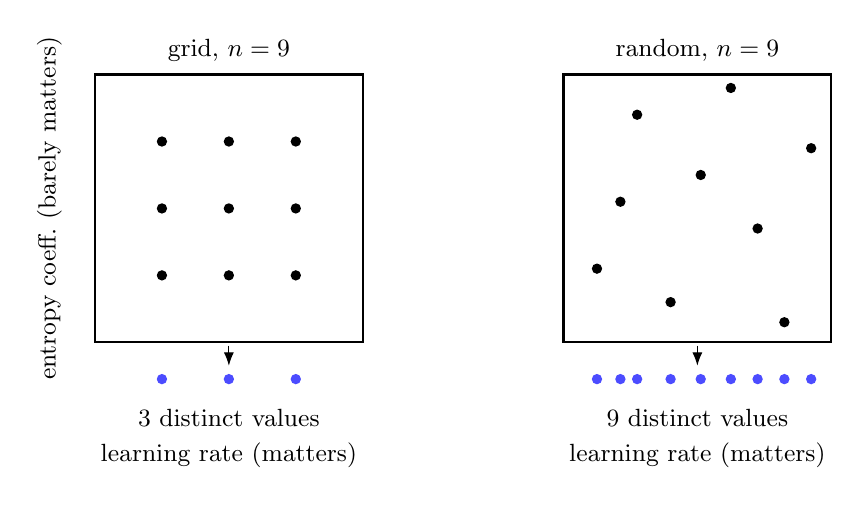
\begin{tikzpicture}[scale=0.85, font=\small]
% left panel: grid
\begin{scope}
\draw[thick] (0,0) rectangle (4,4);
\foreach \x in {1,2,3}
  \foreach \y in {1,2,3}
    \fill (\x,\y) circle (2.2pt);
% projections
\foreach \x in {1,2,3}
  \fill[blue!70] (\x,-0.55) circle (2.2pt);
\draw[-{Latex}] (2,-0.05) -- (2,-0.35);
\node[anchor=north] at (2,-0.85) {3 distinct values};
\node[anchor=south] at (2,4.05) {grid, $n=9$};
\node[rotate=90, anchor=south] at (-0.35,2) {entropy coeff.\ (barely matters)};
\node[anchor=north] at (2,-1.35) {learning rate (matters)};
\end{scope}
% right panel: random
\begin{scope}[xshift=7cm]
\draw[thick] (0,0) rectangle (4,4);
\foreach \p in {(0.5,1.1),(1.1,3.4),(1.6,0.6),(2.05,2.5),(2.5,3.8),(2.9,1.7),(3.3,0.3),(3.7,2.9),(0.85,2.1)}
  \fill \p circle (2.2pt);
\foreach \x in {0.5,1.1,1.6,2.05,2.5,2.9,3.3,3.7,0.85}
  \fill[blue!70] (\x,-0.55) circle (2.2pt);
\draw[-{Latex}] (2,-0.05) -- (2,-0.35);
\node[anchor=north] at (2,-0.85) {9 distinct values};
\node[anchor=south] at (2,4.05) {random, $n=9$};
\node[anchor=north] at (2,-1.35) {learning rate (matters)};
\end{scope}
\end{tikzpicture}
\caption{The projection argument for random search, after
\citet{bergstra2012random}, drawn schematically. When one axis dominates the
objective, only the coverage of that axis's projection (blue) matters. The
same nine trials give the important axis three distinct values under a grid
and nine under random sampling, and random search does not need to know
which axis is important to collect this advantage.}
\label{fig:gridrandom}
\end{figure}

The same point can be made with elementary probability, and the number is
worth carrying around. Suppose ``good'' configurations occupy some fraction
$p$ of the search space, say the top 5 percent. Each uniform random trial
lands in the good region with probability $p$ independently, so the chance
that $n$ trials all miss it is $(1-p)^n$, and
\begin{equation}
\Pr[\text{at least one good trial}] \;=\; 1 - (1-p)^n .
\label{eq:coverage}
\end{equation}
With $p = 0.05$, sixty trials give $1 - 0.95^{60} \approx 0.95$: sixty
random trials find a top-5-percent configuration with 95 percent
probability, in any number of dimensions.

The dimension-free character of
\eqref{eq:coverage} is the honest content of the phrase ``random search
scales'': what it cannot do is exploit structure, so when the good region
is much smaller than 5 percent, or when we want the best of the good region
rather than a member of it, the model-based methods of
Chapter~\ref{sec:bayesian} earn their complexity.

The empirical side of
\citet{bergstra2012random} showed random search matching or beating grid
search on neural-network tuning at a fraction of the cost, and the result
has aged well: fifteen years later, tuning studies in reinforcement
learning still reach for random search as the honest cheap baseline
\citep{eimer2023hyperparameters}, and it remains the recommended floor in
methodological guides \citep{bischl2023hyperparameter}.

\section{Two free upgrades}

Two refinements cost nothing and should be our defaults wherever
plain random sampling appears. First, sample in a transformed space:
learning rates and other scale parameters should be drawn log-uniformly, since
the difference between $10^{-3}$ and $10^{-4}$ matters as much as the
difference between $10^{-4}$ and $10^{-5}$. A uniform draw from
$[10^{-5}, 10^{-2}]$ puts 90 percent of its samples above $10^{-3}$,
crowding into the top decade of the range; a log-uniform draw spends a
third of its budget in each of the three decades. The transform matters
more than any sophistication layered on top of it, and the same logic will
reappear as input warping inside Gaussian-process surrogates
(Chapter~\ref{sec:bayesian}).

Second, replace independent draws with a low-discrepancy sequence (Sobol
points), which spreads samples more evenly than chance and removes the
unlucky clusters and gaps of independent sampling: independent uniform draws
are perfectly happy to put two of nine samples almost on top of each other,
which purchases the same information twice. The gain is modest but free, and
quasi-random initialization is already the default first phase inside
several Bayesian optimization packages.

\section{Respecting the baseline}

Random search has one property that deserves respect when we evaluate our own
product: it is unbiased and easy to reason about. \citet{wan2022bgpbt} found
random search over their full 15-dimensional joint space to be, in their
words, a surprisingly strong baseline on several Brax environments, on par
with or better than the original population-based training on four of seven
tasks; that is our running example's own search space, and the lesson
transfers directly.

When a proposed method fails to beat well-configured
random search at matched compute, the method, not the baseline, is on trial.
That said, model-based methods do beat it when configured sensibly: the
analysis of the 2020 black-box optimization challenge, run on real tuning
problems, found Bayesian optimization entries clearly ahead of random search
across the board \citep{turner2021bayesian}.

Both facts fit in one sentence:
random search is hard to beat when its budget is generous relative to the
difficulty of the space, and clearly beatable when trials are scarce enough
that each one has to be chosen with care. Scarce, expensive trials are our
situation, which is why Chapter~\ref{sec:bayesian} exists.

\section{Adapting the sampler without modeling the objective}

Evolutionary and direct-search methods occupy a middle ground: no fitted
model of the objective, but the sampling distribution adapts. CMA-ES
(covariance matrix adaptation evolution strategy)
maintains a multivariate Gaussian over a continuous search space and, at
each generation, samples a population from it, ranks the samples by
objective value, and updates the Gaussian toward the successful ones: the
mean moves to a weighted average of the best samples, and the covariance is
updated so that directions in which good steps were recently taken become
directions the sampler explores more boldly \citep{hansen2016cmaes}.

Only
the \emph{ranking} of samples enters the update, never the raw objective
values, which buys invariance to any monotone rescaling of the objective, a
genuinely useful robustness when losses are heavy-tailed.

The price is
appetite: covariance adaptation needs generations of populations to learn
the geometry, so CMA-ES is a strong choice when trials are cheap enough to
afford hundreds to thousands of evaluations, when the space is purely
continuous, and when noise is moderate \citep{hansen2016cmaes}. In the
running example's regime of hours-long trials it is mis-matched; in the
Hamiltonian-network regime of minutes-long trials it is a live option.

Differential evolution, the other family member we will need, proposes new
points by recombining coordinate differences of existing population members:
a mutant is formed by adding the scaled difference of two population members
to a third, then crossed with a parent coordinate by coordinate. Its role
for us is as the engine inside DEHB (Chapter~\ref{sec:multifidelity}),
currently one of the most reliable budget-constrained tuners in
reinforcement learning \citep{eimer2023hyperparameters}. The practical
reading: evolutionary machinery earns its place at low fidelities and inside
hybrid methods, not as a standalone tuner for expensive trials, where its
appetite for evaluations collides with our budgets.

\section{The baseline's case, argued from four angles}
\label{sec:mf0-angles}

The chapter's verdict, transforms and Sobol sampling on by default,
random search enthroned as the mandatory baseline, grid retired to a
debugging view, the evolutionary methods wrapped or embedded rather
than built, is modest, which is why it is worth noticing that four
separate arguments underwrite it.

From arithmetic: the two computations of this chapter are one line
each and dimension-free. The exponent $n^{1/d}$ says a grid starves
every axis long before budgets we can afford; the bound
\eqref{eq:coverage} says sixty random trials find the top twentieth
with 95 percent confidence in any dimension. Between them they fix
both the floor's strength and its limit, since nothing in
\eqref{eq:coverage} improves when the good region shrinks or when we
want its best member rather than any member.

From evidence: the floor held up in the two most adversarial arenas
this document has. In the BG-PBT authors' own fifteen-dimensional
space, random search matched or beat the original population methods
on four of seven tasks (Section~\ref{sec:pop-evidence}); in the
outsiders' challenge on real tuning problems, the model-based entries
beat it across the board (Section~\ref{sec:bo-evidence}). The two
results are one fact seen from its two sides: generous budgets make
the floor hard to beat, scarce trials make deliberation pay, and our
studies live on the scarce side.

From operations: random search has no state, no hyperparameters worth
arguing about, no failure modes, and perfect parallelism, which makes
it the one component whose behavior never needs explaining; the log
and Sobol upgrades are free and are inherited by every later method,
since quasi-random points are also the GP searcher's opening phase;
and grid's single virtue, a table a human can read, survives intact
as the two-knob visual sweep.

From decision theory: the baseline's real product is epistemic. Every
verdict in the chapters ahead has the form ``this method beats the
honest cheap alternative at matched budget,'' and that sentence is
only checkable if the honest cheap alternative is permanently
installed in the validation suite. Carrying it costs nothing;
dropping it would convert every later claim from a measurement into
an opinion.

The falsification here runs in both directions. The chapter's own
positive claims are the cheapest in the document to test, the same
searcher with and without the log transform on a pinned task settles
the transform's value in an afternoon, and the chapter's main export
is the standing criterion the rest of the document is judged by: any
searcher that cannot beat the upgraded floor at matched budget, with
seeds and uncertainty reported, is not shipped.

\begin{decisions}
\noindent\textbf{Decisions from this chapter.} For each method: what it
is in one sentence, and whether it goes in the package.
\begin{itemize}[leftmargin=1.3em, itemsep=2pt]
\item \textbf{Log-scale and Sobol sampling} (include, days of work).
Drawing scale-type knobs on a log scale, and drawing the opening batch
from a scrambled Sobol sequence rather than independently. An
engineering default, not a theorem: the log transform applies to knobs
that span decades (learning rates, coefficients, step sizes) and not to
ordinals or categories, and Sobol's even coverage is a claim about
initialization batches, where it is also the GP searcher's opening
phase anyway. Two caveats worth carrying: scrambling matters, since an
unscrambled sequence's low-order points are visibly structured, and at
budgets of a handful of trials the difference from independent sampling
is below the noise we are measuring against.
\item \textbf{Random search} (include, trivial). Not as a product
feature but as the mandatory baseline in our validation suite: any
searcher that cannot beat it at matched budget is not shipped. The
arithmetic of \eqref{eq:coverage} is why it is harder to beat than its
reputation suggests.
\item \textbf{Grid search} (exclude as a search method). Keep only as a
debugging utility for two-knob visual sweeps; Figure~\ref{fig:gridrandom}
is the entire case against it as a tuner.
\item \textbf{CMA-ES} (include by wrapping an existing implementation,
low priority). Only competitive when a study can afford hundreds of
cheap, continuous trials, which for us means the Hamiltonian-network
regime and nothing else. Building it ourselves would buy nothing.
\item \textbf{Differential evolution} (no standalone entry). It enters
the package only inside DEHB in Chapter~\ref{sec:multifidelity}.
\end{itemize}
\end{decisions}

\section{What would overturn these verdicts}

The floor baseline is structural, not empirical: if the GP searcher
cannot beat log-scale Sobol at matched budget on the pinned tasks of
Chapter~\ref{sec:validation}, it is demoted and this chapter
rewritten. CMA-ES's inclusion is conditional on the wrap remaining
thin; if the dependency becomes unmaintained or the adapter requires
ongoing surgery, the verdict changes to exclude and the register
records it. Grid search's debug-view limit holds unless a colleague
requests it as a search method with a use case the decision boxes
did not consider, at which point the box is reopened.

\chapter{Model-based search: Bayesian optimization and its relatives}
\label{sec:bayesian}

Random search treats trial fifty exactly like trial one: it has learned
nothing. When each trial costs GPU-hours, that indifference is expensive,
and it pays to think hard between trials. Bayesian optimization (BO) spends
that thought in two steps: fit a probabilistic model of the objective from
the trials seen so far (the \emph{surrogate}), then choose the next
configuration by maximizing an \emph{acquisition function} that scores
candidate points by how useful evaluating them would be. The surrogate is
cheap to evaluate, so the inner maximization can afford thousands of
candidate evaluations to decide where to spend one real trial. Modern
references are the book by \citet{garnett2023bayesoptbook} and the survey by
\citet{shahriari2016taking}; here we develop the machinery far enough that
the design choices in our product are not acts of faith, starting from the
question the surrogate must answer: after eight trials of the running
example, what do we believe about the loss at a learning rate we have never
tried, and how sure are we?

\section{Gaussian process surrogates}
\label{sec:gp}

The default surrogate is a Gaussian process (GP), and its entire content is
one modeling assumption stated positively: we model the objective $f$ as a
random function such that any finite collection of values
$(f(\config_1), \dots, f(\config_n))$ is jointly Gaussian, with prior mean
zero and covariance given by a kernel,
$\operatorname{Cov}[f(\config), f(\config')] = k(\config, \config')$. The
kernel is where all the prior knowledge lives: it says how similar the
objective's values at two configurations should be as a function of how far
apart the configurations are. The common default, and ours, is the
Mat\'ern-5/2 kernel with a lengthscale per dimension,
\begin{equation}
k(\config, \config')
= \sigma_f^2 \left( 1 + \sqrt{5}\,\rho + \tfrac{5}{3}\rho^2 \right)
  e^{-\sqrt{5}\,\rho},
\qquad
\rho^2 = \sum_{j=1}^{d} \frac{(\lambda_j - \lambda'_j)^2}{\ell_j^2},
\label{eq:matern}
\end{equation}
which produces functions that are twice differentiable but not infinitely
smooth, a better match for loss surfaces than the very smooth squared
exponential \citep{rasmussen2006gaussian}. Each lengthscale $\ell_j$ has a
direct reading: it is the distance along axis $j$ over which the objective's
values decorrelate. A long lengthscale on the entropy-coefficient axis says
that moving the entropy coefficient barely changes the loss.

It is worth pausing on why the model is nonparametric, because the
obvious alternative is one every applied statistician has fit. Response
surface methodology would posit a global parametric form, a quadratic in
the knobs, and estimate its coefficients by least squares. That imposes
one curvature on the entire space: the model must believe the loss bends
the same way near $10^{-5}$ as near $10^{-2}$, and eight trials estimating
a fifteen-dimensional quadratic are hopeless anyway (the quadratic alone
has over a hundred coefficients). The kernel assumption is weaker and
better matched to what we actually know: not the shape of the surface,
only that configurations close together perform similarly, with
``close'' learned per axis from the data. The GP is what Bayesian
regression becomes when the parametric form is dropped and only that
smoothness belief is kept; the price is that predictions lean on nearby
data rather than on a global formula, which is exactly the right
epistemic posture for a surface we know nothing else about.

We assume observations are the true objective plus Gaussian noise,
$y_i = f(\config_i) + \varepsilon_i$ with
$\varepsilon_i \sim \N(0, \sigma^2)$, which is our stand-in for seed
variation; it is a modeling choice, adopted because it keeps every formula
below in closed form, and Section~\ref{sec:gp-practical} returns to what to
do when the noise is visibly not Gaussian. Under these assumptions the
prediction problem solves itself by pure linear algebra. The observed vector
$\mathbf{y} = (y_1, \dots, y_n)$ and the unknown value $f(\config)$ at a new
point are jointly Gaussian,
\begin{equation}
\begin{pmatrix} \mathbf{y} \\ f(\config) \end{pmatrix}
\sim \N\!\left(
\mathbf{0},
\begin{pmatrix}
\mathbf{K} + \sigma^2 \mathbf{I} & \mathbf{k}(\config) \\
\mathbf{k}(\config)^\top & k(\config, \config)
\end{pmatrix}
\right),
\qquad
\mathbf{K}_{ij} = k(\config_i, \config_j),
\quad
\mathbf{k}(\config)_i = k(\config_i, \config),
\label{eq:joint}
\end{equation}
and the standard formula for conditioning one block of a Gaussian on
another (condition the second block on the first) gives the posterior at
$\config$ as another Gaussian,
\begin{equation}
\mu_n(\config) = \mathbf{k}(\config)^\top
\left( \mathbf{K} + \sigma^2 \mathbf{I} \right)^{-1} \mathbf{y},
\qquad
s_n^2(\config) = k(\config, \config) - \mathbf{k}(\config)^\top
\left( \mathbf{K} + \sigma^2 \mathbf{I} \right)^{-1} \mathbf{k}(\config)
\label{eq:gp}
\end{equation}
\citep{rasmussen2006gaussian}. Readers who know kriging from spatial
statistics or Bayesian linear regression from econometrics are on home
ground here: \eqref{eq:gp} is exactly that conditioning, with the kernel
playing the role of the spatial covariance function.

The two formulas
carry the whole story, and they are worth reading term by term. The posterior mean is a weighted
combination of the observed values, with weights
$\mathbf{k}(\config)^\top (\mathbf{K} + \sigma^2 \mathbf{I})^{-1}$ set by
similarity under the kernel: observations near $\config$ (as measured in
lengthscale units) dominate the prediction.

The posterior variance starts
from the prior variance $k(\config,\config)$ and \emph{subtracts} a term
that grows as data approaches $\config$; at fixed kernel
hyperparameters nothing about the observed \emph{values} appears in it,
only the observed \emph{locations}, so the model knows where it is
ignorant before it knows what the answer is. The qualifier is not
decoration: once the lengthscales and the noise variance are estimated
from the data by \eqref{eq:mll}, the observed values do influence the
variance, through the fitted hyperparameters rather than through the
conditioning formula.

The noise term $\sigma^2 \mathbf{I}$ deserves its own sentence: with
$\sigma^2 = 0$ the posterior mean passes exactly through every
observation, treating each score as gospel, while $\sigma^2 > 0$ turns
interpolation into smoothing, letting the mean pass \emph{near} noisy
scores instead of through them. Readers who know ridge regression will
recognize the mechanism, since $(\mathbf{K} + \sigma^2\mathbf{I})^{-1}$
applies precisely ridge's shrinkage, with the noise variance as the
regularization constant; estimating $\sigma^2$ from the data by
\eqref{eq:mll} below is what lets the model decide for itself how much
of the spread in RL returns is signal and how much is seed luck.

Figure~\ref{fig:gp} shows the shape this produces on the running example's
learning-rate axis: the band of uncertainty is pinched near the trials we
have paid for and swells between and beyond them, which is exactly the
information an acquisition function needs.

\begin{figure}[t]
\centering
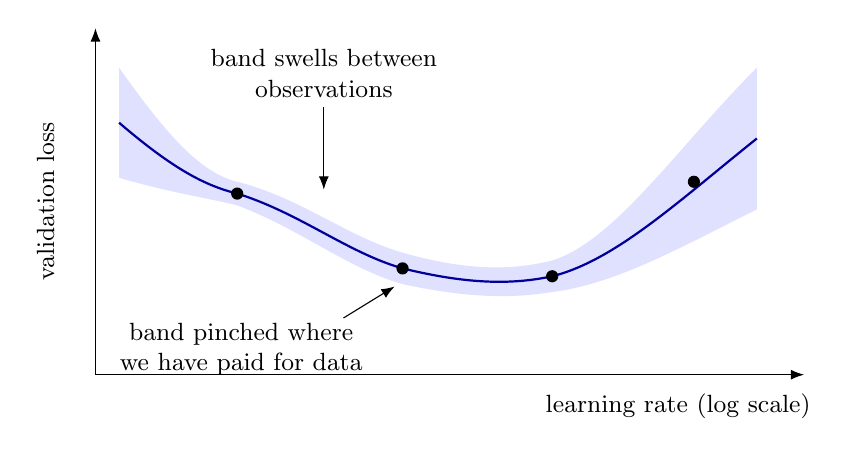
\begin{tikzpicture}[scale=1.0, font=\small]
% axes
\draw[-{Latex}] (0,0) -- (9,0);
\node[anchor=north] at (7.4,-0.12) {learning rate (log scale)};
\draw[-{Latex}] (0,0) -- (0,4.4);
\node[rotate=90, anchor=south] at (-0.4,2.2) {validation loss};
% uncertainty band (upper then lower reversed)
\fill[blue!12]
  (0.3,3.9) .. controls (1.0,2.9) and (1.4,2.55) .. (1.8,2.45)
  .. controls (2.6,2.25) and (3.2,1.75) .. (3.9,1.55)
  .. controls (4.6,1.35) and (5.2,1.30) .. (5.8,1.45)
  .. controls (6.6,1.70) and (7.4,2.9) .. (8.4,3.9)
  -- (8.4,2.1)
  .. controls (7.4,1.6) and (6.6,1.15) .. (5.8,1.05)
  .. controls (5.2,0.95) and (4.6,1.00) .. (3.9,1.15)
  .. controls (3.2,1.35) and (2.6,1.85) .. (1.8,2.15)
  .. controls (1.4,2.25) and (1.0,2.3) .. (0.3,2.5)
  -- cycle;
% mean
\draw[thick, blue!60!black]
  (0.3,3.2) .. controls (1.0,2.6) and (1.4,2.4) .. (1.8,2.3)
  .. controls (2.6,2.05) and (3.2,1.55) .. (3.9,1.35)
  .. controls (4.6,1.18) and (5.2,1.12) .. (5.8,1.25)
  .. controls (6.6,1.45) and (7.4,2.2) .. (8.4,3.0);
% data points
\fill (1.8,2.3) circle (2.2pt);
\fill (3.9,1.35) circle (2.2pt);
\fill (5.8,1.25) circle (2.2pt);
\fill (7.6,2.45) circle (2.2pt);
% annotations
\draw[-{Latex}] (3.15,0.72) -- (3.8,1.12);
\node[anchor=north, align=center] at (1.85,0.78) {band pinched where\\we have paid for data};
\draw[-{Latex}] (2.9,3.4) -- (2.9,2.35);
\node[anchor=south, align=center] at (2.9,3.4) {band swells between\\observations};
\end{tikzpicture}
\caption{A Gaussian-process posterior on the running example's
learning-rate axis after four trials (schematic illustration of the
mechanism, not measured data). The mean~\eqref{eq:gp} passes near the
observations; the shaded one-standard-deviation band shows
$\mu_n \pm s_n$, which is pinched near observed points and grows away
from them. The figure is drawn in the low-noise regime for legibility:
with $\sigma^2 > 0$ the mean does not interpolate exactly and the
variance at an observed location stays strictly positive, and only in
the noiseless limit $\sigma^2 \to 0$ does the band close completely.
Given the kernel hyperparameters, the posterior variance depends only on
\emph{where} we have evaluated, not on the values we saw, so the model
maps its own ignorance; once those hyperparameters are themselves fitted
by marginal likelihood (below), the observed values re-enter the
variance indirectly through them.}
\label{fig:gp}
\end{figure}

The kernel hyperparameters (the lengthscales $\ell_j$, signal variance
$\sigma_f^2$, and noise $\sigma^2$) are learned by maximizing the marginal
likelihood of the data,
\begin{equation}
\log p(\mathbf{y} \mid \boldsymbol{\ell}, \sigma_f, \sigma)
= -\tfrac{1}{2} \mathbf{y}^\top (\mathbf{K} + \sigma^2 \mathbf{I})^{-1}
   \mathbf{y}
  \;-\; \tfrac{1}{2} \log \det (\mathbf{K} + \sigma^2 \mathbf{I})
  \;-\; \tfrac{n}{2} \log 2\pi ,
\label{eq:mll}
\end{equation}
whose two data-dependent terms pull in opposite directions: the first
rewards kernels under which the observed values are unsurprising (fit), the
second penalizes kernels that could explain anything (complexity), so
maximizing the sum performs a built-in Occam trade-off
\citep{rasmussen2006gaussian}.

This is how a GP quietly performs the
sensitivity analysis that grid search cannot: if the data can be explained
with a very long lengthscale on some axis, the likelihood prefers it, and
that axis is effectively switched off. The fitted numbers are worth
reading, not just using: if the running example's model learns a
lengthscale of half a decade on the log learning-rate axis, then trials
a decade apart are nearly independent evidence and the axis needs dense
coverage; a fitted lengthscale of five decades says the axis is
effectively flat and the search can spend its trials elsewhere.

The $n \times n$ solve in
\eqref{eq:gp} and \eqref{eq:mll} costs $O(n^3)$ time, irrelevant at our
trial counts (tens to low hundreds) but a real constraint for methods that
model learning curves point by point, a fact that returns in
Chapter~\ref{sec:multifidelity}.

\subsection{What actually goes wrong in practice}
\label{sec:gp-practical}

Two practical amendments matter more than any exotic kernel choice, and
both are the same move we made for random search: respect the data's
geometry. First, inputs should be warped: search axes like learning rate
live on a log scale, and beyond fixed transforms it helps to learn a
monotone warping of each axis (HEBO uses a Kumaraswamy distribution
function per axis) so that the objective looks stationary to the kernel;
a kernel with one lengthscale per axis assumes the objective wiggles at
the same rate everywhere along that axis, and warping is how we make that
assumption true rather than hoping it holds.

Second, outputs should be
transformed toward Gaussianity by a power transform, because raw losses are
often heavy-tailed and heteroscedastic: one diverged trial with a loss of
$10^{6}$ will otherwise dominate the fit of \eqref{eq:mll} and flatten the
model's view of the interesting region.

HEBO's authors open their paper
with hypothesis tests on 108 real tuning tasks showing that
heteroscedasticity and non-stationarity are the rule, not the exception,
and HEBO won the NeurIPS 2020 black-box optimization challenge with exactly
these amendments plus one more hedge: instead of trusting any single
rule for choosing the next trial, HEBO scores candidates by three
standard such rules at once (the acquisition functions of the next
section) and picks candidates that no rival beats on all three
\citep{cowenrivers2022hebo, turner2021bayesian}. The lesson for
implementers is encouraging: the wins come from respecting the data's
geometry, not from acquisition novelty.

\section{Acquisition functions}
\label{sec:acquisition}

The surrogate summarizes belief; the acquisition function turns belief into
a decision, and the decision has a tension in it. Sampling where the mean
$\mu_n$ is best exploits what we know; sampling where the variance $s_n^2$
is largest explores what we do not. Every acquisition function is a
different exchange rate between the two.

\subsection{Expected improvement, derived and then broken}

Expected improvement (EI), the traditional default, scores a candidate by
the expected amount by which it beats the best value seen so far. Write
$f^{\star}$ for the incumbent value (in minimization). If we evaluate at
$\config$ and observe $f(\config)$, the improvement is
$\max(f^{\star} - f(\config), 0)$: the amount by which we beat the
incumbent, or zero if we fail to. An economist will recognize the shape
immediately: this is an option payoff with strike $f^{\star}$, and EI is
its expected value under the posterior, so Bayesian optimization spends
its trials the way one prices options, paying for upside while the
downside is capped at the cost of the trial.

Under the posterior \eqref{eq:gp},
$f(\config) \sim \N(\mu_n, s_n^2)$, and the expectation of the improvement
has a closed form. Substituting $z = (f - \mu_n)/s_n$ and writing
$u = (f^{\star} - \mu_n)/s_n$ for the incumbent's position in posterior
standard units,
\begin{equation}
\alpha_{\mathrm{EI}}(\config)
= \int_{-\infty}^{f^{\star}} (f^{\star} - f)\,
  \frac{1}{s_n}\varphi\!\Big(\frac{f-\mu_n}{s_n}\Big)\, df
= s_n \int_{-\infty}^{u} (u - z)\, \varphi(z)\, dz
= s_n \left[ u\,\Phi(u) + \varphi(u) \right],
\label{eq:ei-derive}
\end{equation}
using $\int_{-\infty}^{u} \varphi(z)\,dz = \Phi(u)$ and
$\int_{-\infty}^{u} z\,\varphi(z)\,dz = -\varphi(u)$, the latter because
$\varphi'(z) = -z\varphi(z)$. Rearranged into its usual form,
\begin{equation}
\alpha_{\mathrm{EI}}(\config)
= \left( f^{\star} - \mu_n(\config) \right) \Phi(u)
  + s_n(\config)\, \varphi(u),
\qquad
u = \frac{f^{\star} - \mu_n(\config)}{s_n(\config)},
\label{eq:ei}
\end{equation}
with $\varphi$ and $\Phi$ the standard normal density and distribution
function \citep{jones1998efficient}. The two terms are the two halves of
the tension made explicit: the first rewards a promising mean (how much
better than the incumbent we expect to be, times the probability of being
better at all), the second rewards uncertainty, and the balance between
them is automatic, with no exploration knob to tune.

A small worked case shows the balance operating, and it is worth doing
once by hand. Suppose the incumbent loss in the running example is
$f^{\star} = 0.60$. Candidate A sits in unexplored territory: the
posterior says $\mu_n = 0.62$, $s_n = 0.05$, so $u = -0.4$, and
\eqref{eq:ei} gives
$\alpha_{\mathrm{EI}} = (-0.02)(0.345) + (0.05)(0.368) \approx 0.012$.
Candidate B sits next to the incumbent: $\mu_n = 0.59$, $s_n = 0.005$, so
$u = 2$, and
$\alpha_{\mathrm{EI}} = (0.01)(0.977) + (0.005)(0.054) \approx 0.010$.

Candidate A has the \emph{worse} expected loss, yet EI ranks it slightly
ahead, because its wide posterior leaves real probability of a large
improvement, while candidate B can improve on the incumbent by at most a
hair. That preference for informative gambles over safe pennies is the
entire personality of EI, and Figure~\ref{fig:ei} draws where it comes
from: the acquisition is the mass of the posterior lying below the
incumbent line, weighted by how far below it lies.

\begin{figure}[t]
\centering
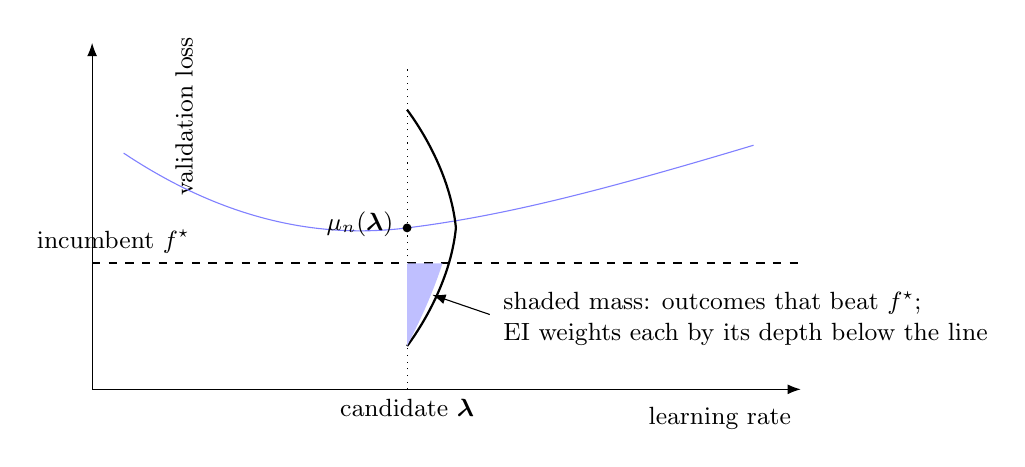
\begin{tikzpicture}[scale=1.0, font=\small]
\draw[-{Latex}] (0,0) -- (9,0) node[below left=1mm and 0mm] {learning rate};
\draw[-{Latex}] (0,0) -- (0,4.4) node[rotate=90, above left=2mm and -14mm] {validation loss};
% incumbent line
\draw[dashed, thick] (0,1.6) -- (9,1.6) node[pos=0.03, above, font=\small] {incumbent $f^{\star}$};
% posterior mean curve (light)
\draw[blue!50]
  (0.4,3.0) .. controls (1.6,2.2) and (2.8,1.9) .. (4.0,2.05)
  .. controls (5.2,2.2) and (6.4,2.5) .. (8.4,3.1);
% candidate location
\draw[dotted] (4.0,0) node[below] {candidate $\config$} -- (4.0,4.1);
% rotated gaussian at x=4 centered at mu=2.05, drawn as profile to the right
\draw[thick]
  (4.0,3.55) .. controls (4.15,3.35) and (4.55,2.75) .. (4.62,2.05)
  .. controls (4.55,1.35) and (4.15,0.75) .. (4.0,0.55);
% shade improvement region: part of bell below y=1.6
\fill[blue!25]
  (4.0,1.6) -- (4.45,1.6)
  .. controls (4.3,1.15) and (4.15,0.85) .. (4.0,0.55) -- cycle;
\node[anchor=west, align=left] at (5.1,0.9)
  {shaded mass: outcomes that beat $f^{\star}$;\\
   EI weights each by its depth below the line};
\draw[-{Latex}] (5.05,0.95) -- (4.32,1.2);
\fill (4.0,2.05) circle (1.6pt);
\node[anchor=east] at (3.95,2.1) {$\mu_n(\config)$};
\end{tikzpicture}
\caption{What expected improvement measures (schematic). At the candidate,
the posterior over the unknown loss is the sideways bell curve. Only the
shaded tail below the incumbent line counts as improvement, and
\eqref{eq:ei} is exactly this tail's mass weighted by its depth. When the
whole bell sits far above the line, the shaded region, and with it EI and
its gradient, vanishes; that observation is the doorway to the numerical
failure discussed next.}
\label{fig:ei}
\end{figure}

Now the flaw, which is not conceptual but floating-point, and which
matters because we will inherit it the day we ship a naive
implementation. Once a decent incumbent exists, most of the search space
has $\mu_n$ far above $f^{\star}$, so $u$ is a large negative number. For
large negative $u$ the standard tail expansion of $\Phi$ gives
$\alpha_{\mathrm{EI}} \approx s_n \varphi(u)/u^2$, and $\varphi(u)$ decays
like $e^{-u^2/2}$: at $u = -6$ the acquisition is already of order
$10^{-10} s_n$, and near $u \approx -38$ the density $\varphi(u)$ leaves
the range of double-precision numbers entirely, so \eqref{eq:ei} evaluates
to exactly zero, its gradient with it. A value of $u = -6$ is not exotic;
it just means the posterior mean is six posterior standard deviations
worse than the incumbent, which describes most of the domain once the
search has found anything good. In that regime multi-restart gradient
ascent on the acquisition degenerates into random search among its own
starting points.

\citet{ament2023logei} analyze this failure, show that
the affected region grows with observations, dimensions, and constraints,
and repair it by optimizing numerically careful $\log$ transforms of the
whole EI family (analytic, batch, constrained, and hypervolume variants):
$\log \alpha_{\mathrm{EI}}$ is computed directly from stable asymptotic
expansions rather than by taking the logarithm of an underflowed number,
and smooth approximations replace the hard maximum inside the Monte
Carlo versions, the sampling-based batch variants that arrive later in
this section. The logarithm does not change where the maxima are; it changes
whether an optimizer can find them, because gradients of order
$10^{-300}$ become gradients of order one.

The repaired acquisitions
match or beat more elaborate alternatives across standard benchmarks,
which suggests much of EI's mixed reputation was numerics all along. Our
implementation should treat the LogEI variants as the default and never
optimize raw EI.

\subsection{The rest of the family, and when we need it}

A different family spends its budget on information rather than
improvement: predictive entropy search values a candidate by how much its
observation would shrink uncertainty about the optimum's location
\citep{hernandez2014pes}, max-value entropy search replaces the location
(a $d$-dimensional object) with the optimum's value (a scalar), making the
computation far cheaper \citep{wang2017mes}, and joint entropy search
conditions on fantasized optimal input-output pairs to capture both at
once \citep{hvarfner2022jes}.

These acquisitions are elegant and
occasionally worth their cost on very expensive problems, but given the
LogEI result above we treat them as optional extras rather than defaults;
\citet{frazier2018tutorial} is the standard tour of the whole acquisition
zoo, including the knowledge gradient that Chapter~\ref{sec:moo} meets
again in multi-objective form.

Two families beyond EI matter for us directly. Upper confidence bound
(UCB) style rules score a candidate by an optimistic quantile of the
posterior,
\begin{equation}
\alpha_{\mathrm{UCB}}(\config)
= \mu_n(\config) - \beta^{1/2}\, s_n(\config)
\label{eq:ucb}
\end{equation}
for minimization: pretend every point is as good as its posterior allows
at confidence level $\beta$, then pick the best pretend value. Larger
$\beta$ explores harder. The rule comes with regret guarantees under
GP-bandit assumptions, with $\beta$ growing slowly over time so that no
region is starved forever \citep{srinivas2010gaussian}, and it extends
naturally to the time-varying setting that population-based methods
inhabit; PB2, a population-based tuner taught in
Chapter~\ref{sec:population}, uses exactly such a rule, so
the formula is worth remembering.

Noise-aware variants of EI stop pretending the incumbent value
$f^{\star}$ is known, and the reason they must is a bias economists
teach under its own name. With noisy observations the ``best value
seen'' is the \emph{minimum of noisy draws}, and the minimum of noisy
draws is optimistically biased: the trial that reported the best return
in the running example is disproportionately likely to be a decent
configuration that also drew a lucky seed. This is the winner's curse,
and plugging the lucky number into \eqref{eq:ei} as $f^{\star}$
transmits the curse to every later decision: the reported incumbent is
better than the true incumbent, so genuine improvements look smaller
than they are, the acquisition under-rewards them, and the search
stalls defending a score that no configuration, including the
incumbent itself, can reproduce.

The repair is to stop conditioning on
the noisy draws and integrate over what the true values might be. Let
$f(\config_{1:n})$ be the (unknown) true objective values at the
evaluated points; the noisy-EI acquisition is
\begin{equation}
\alpha_{\mathrm{NEI}}(\config)
= \E\!\left[ \max\!\Big( \min_{i \le n} f(\config_i) - f(\config),\; 0
\Big) \right],
\label{eq:nei}
\end{equation}
where the expectation runs over the \emph{joint} posterior of
$f(\config)$ and $f(\config_{1:n})$: the incumbent value inside the
expectation is the true best, not the lucky observed best, and the
average over the posterior prices the luck out.

The integral has no
closed form and is estimated by Monte Carlo, jointly sampling the true
values at old and candidate points; this is the formalization of the
approach used in production at Meta and now standard in BoTorch
\citep{letham2019noisyei, balandat2020botorch}, and its log-stabilized
version inherits the LogEI repair \citep{ament2023logei}.
Reinforcement learning returns and effective-sample-size measurements
are noisy enough that a tuner without the noise-aware acquisition can
waste budget refining estimates of points the GP already knows about
rather than exploring genuinely new candidates, so we ship the
noise-aware variant by default. A user whose observations are nearly
deterministic may switch it off, but RL and sampling workloads keep
it on.

Batch and asynchronous proposals fall out of the same Monte Carlo
formulation, and they answer the wall-clock concern of
Section~\ref{sec:costmodel}. To propose $q$ points jointly, one optimizes
the expected improvement of the \emph{best} of the $q$, which
automatically spreads the batch out (two candidates next to each other
mostly duplicate each other's improvement, so the joint objective prefers
diversity without any explicit diversity penalty).

To propose while $k$
trials are still running, one conditions on their unknown outcomes by
sampling them from the posterior (so-called fantasies) and averages the
resulting decisions \citep{balandat2020botorch}. This is the machinery
that lets model-based search keep a pool of workers busy rather than
idling between sequential suggestions, and it is a hard requirement for
us, not a luxury.

One mechanical detail completes the picture, because ``maximize the
acquisition'' is itself an optimization problem and its failure mode is
the one LogEI fixed. In continuous spaces the standard recipe scores a
few thousand quasi-random candidates (Sobol points again), keeps the
best handful, and polishes each by gradient ascent, which is possible
because $\mu_n$ and $s_n$ in \eqref{eq:gp} are differentiable in
$\config$ and the Monte Carlo acquisitions are built to be
differentiated \citep{balandat2020botorch}. In mixed spaces the
gradient steps apply to the continuous coordinates and local moves to
the discrete ones, the interleaving that Casmopolitan formalizes
(Section~\ref{sec:highdim}). The polish step is exactly where a flat,
underflowed acquisition strands the optimizer at its starting points,
which is why the numerics of the previous subsection are an
engineering requirement rather than a refinement.

\section{Density-ratio and tree-based alternatives}
\label{sec:tpe}

The tree-structured Parzen estimator (TPE) inverts the modeling question,
and the inversion is worth deriving because it explains both TPE's
strengths and its blind spot. Instead of modeling $p(y \mid \config)$ as
the GP does, TPE splits the observed trials at the $\gamma$-quantile of
their scores $y^{\star}$ (say the best 25 percent versus the rest) and
fits kernel density estimates to the two groups of \emph{configurations}:
$\ell(\config)$ for configurations that scored well, $g(\config)$ for the
rest \citep{bergstra2011tpe}. New candidates are proposed where the ratio
$\ell(\config)/g(\config)$ is largest: where good trials cluster and bad
trials are rare (Figure~\ref{fig:tpe-fig}).

The connection to EI is not a
heuristic. Under TPE's model, $p(\config \mid y)$ equals $\ell(\config)$
when $y < y^{\star}$ and $g(\config)$ otherwise, so by Bayes' rule the
marginal is
$p(\config) = \gamma\, \ell(\config) + (1-\gamma)\, g(\config)$, and the
expected improvement below the threshold becomes
\begin{equation}
\alpha_{\mathrm{EI}}(\config)
= \int_{-\infty}^{y^{\star}} (y^{\star} - y)\,
  \frac{p(\config \mid y)\, p(y)}{p(\config)} \, dy
\;=\; \frac{\ell(\config)\int_{-\infty}^{y^{\star}}(y^\star - y)p(y)\,dy}
  {\gamma\, \ell(\config) + (1-\gamma)\, g(\config)}
\;\propto\;
\left( \gamma + (1 - \gamma)\, \frac{g(\config)}{\ell(\config)}
\right)^{-1},
\label{eq:tpe}
\end{equation}
since the integral in the numerator does not depend on $\config$. The
right-hand side is a monotone increasing function of
$\ell(\config)/g(\config)$: maximizing the density ratio \emph{is}
maximizing EI under this model \citep{bergstra2011tpe}.

What the model
gives up is visible in the same derivation: the densities are typically
factorized per coordinate, so the ratio cannot represent ``this learning
rate is good only when the batch size is large,'' an interaction a GP
kernel captures without effort.

\begin{figure}[t]
\centering
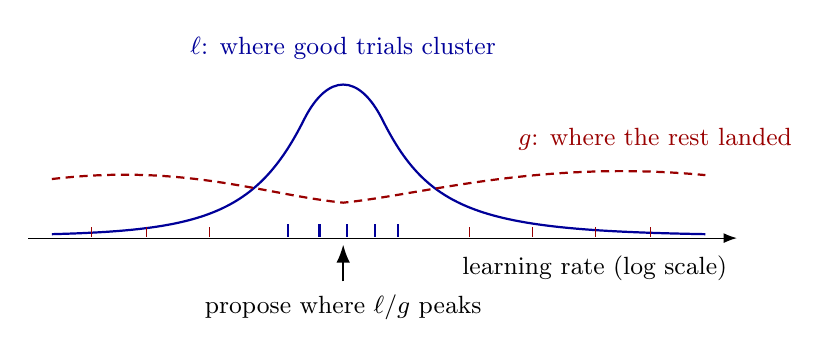
\begin{tikzpicture}[scale=1.0, font=\small]
\draw[-{Latex}] (0,0) -- (9,0) node[below left=1mm and 0mm] {learning rate (log scale)};
% good density l(x): concentrated bump
\draw[thick, blue!60!black]
  (0.3,0.05) .. controls (2.2,0.1) and (2.9,0.3) .. (3.5,1.5)
  .. controls (3.8,2.1) and (4.2,2.1) .. (4.5,1.5)
  .. controls (5.1,0.3) and (5.8,0.1) .. (8.6,0.05);
\node[blue!60!black, anchor=south] at (4.0,2.15) {$\ell$: where good trials cluster};
% bad density g(x): broad
\draw[thick, red!60!black, densely dashed]
  (0.3,0.75) .. controls (2.0,0.95) and (3.0,0.55) .. (4.0,0.45)
  .. controls (5.0,0.55) and (6.5,1.0) .. (8.6,0.8);
\node[red!60!black, anchor=west] at (6.1,1.25) {$g$: where the rest landed};
% ratio argmax marker
\draw[-{Latex}, thick] (4.0,-0.55) -- (4.0,-0.08);
\node[anchor=north] at (4.0,-0.6) {propose where $\ell/g$ peaks};
% data ticks
\foreach \x in {3.3,3.7,4.05,4.4,4.7} \draw[blue!60!black, thick] (\x,0.02) -- (\x,0.18);
\foreach \x in {0.8,1.5,2.3,5.6,6.4,7.2,7.9} \draw[red!60!black] (\x,0.02) -- (\x,0.14);
\end{tikzpicture}
\caption{TPE's view of the running example's learning-rate axis
(schematic). Trials are split at a score quantile; the configurations of
the good fraction (solid ticks) get density $\ell$, the rest (dashed
ticks) get $g$, and the next candidate maximizes $\ell/g$, which
by~\eqref{eq:tpe} is the same as maximizing expected improvement under
TPE's model. The construction never represents interactions between axes;
that is the price of its speed and its ease with categorical and
conditional parameters.}
\label{fig:tpe-fig}
\end{figure}

Three properties make TPE the workhorse of Optuna, the open-source
tuning library where sampler development is most active (its record is
audited in Chapter~\ref{sec:libraries}). It
handles conditional (tree-structured) spaces natively, because densities
are fit per branch of the configuration tree; it tolerates categorical
and integer parameters without kernel gymnastics, since a kernel density
over a finite set is just a weighted histogram; and its cost grows gently
with both dimension and trial count, with none of the $O(n^3)$ algebra
of~\eqref{eq:gp}. Its weakness is the flip side of the factorized
densities above: blindness to interactions, and in low dimensions with
smooth objectives a GP squeezes more out of each trial. The recent
tutorial by \citet{watanabe2023tpe} documents the many small design
choices (bandwidths, splitting quantile, prior weight) that separate a
good TPE from a poor one; since Optuna implements these carefully,
wrapping Optuna's sampler is more sensible than reimplementing TPE
ourselves.

SMAC replaces the GP with a random forest surrogate, which natively
digests mixed and conditional spaces and yields uncertainty from the
spread across trees \citep{lindauer2022smac3}. Forest surrogates are less
sample-efficient than GPs on smooth low-dimensional problems but degrade
gracefully on the awkward spaces where GPs struggle, and SMAC3 pairs the
surrogate with multi-fidelity racing (Chapter~\ref{sec:multifidelity}).
We cite it here both as an algorithmic reference point and because it is
the tuner that \citet{wan2022bgpbt} used as their sequential BO baseline.

\section{High-dimensional and mixed spaces}
\label{sec:highdim}

Vanilla GP BO has a reputation for failing beyond ten or twenty
dimensions, which would be disqualifying for the running example's
fifteen. The reputation is only half deserved, and the recent literature
sorts out which half; the sorting matters to us because it changes what
we build first.

The mechanism behind the failures is worth stating before the fixes. In
high dimension, with standard lengthscale priors, the fitted GP tends
toward one of two degenerate postures: lengthscales so short that every
observation is an island (posterior variance is high everywhere, and the
acquisition chases pure exploration into the corners), or a fit that
contorts itself around noise. Each published fix restricts the model in a
different way, and each restriction is a bet about the objective.

TuRBO bets that good local models beat bad global ones. It abandons the
global search problem and maintains local trust regions: boxes around
good points, inside each of which an independent BO runs with its own GP
(Figure~\ref{fig:turbo}). A region's side length grows after runs of
successes (the local model is trustworthy, let it see further) and
shrinks after runs of failures (the local model is misleading, tighten
the box); a region that shrinks below a floor is abandoned and restarted
elsewhere, and a bandit allocates trials across regions
\citep{eriksson2019turbo}. This concentrates samples where the model has
earned trust and scales to hundreds of dimensions; it is the backbone
that BG-PBT adapts for population training (Chapter~\ref{sec:population}),
which is the specific reason this document cares about its details.

\begin{figure}[t]
\centering
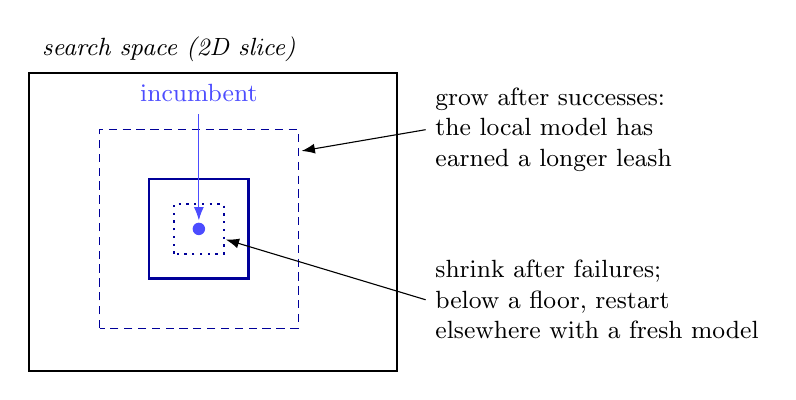
\begin{tikzpicture}[scale=0.9, font=\small]
\draw[thick] (0,0) rectangle (5.2,4.2);
\node[anchor=south west, font=\small\itshape] at (0.05,4.22) {search space (2D slice)};
% incumbent
\fill[blue!70] (2.4,2.0) circle (2.5pt);
% trust region boxes
\draw[blue!60!black, thick] (1.7,1.3) rectangle (3.1,2.7);
\draw[blue!60!black, densely dashed] (1.0,0.6) rectangle (3.8,3.4);
\draw[blue!60!black, dotted, thick] (2.05,1.65) rectangle (2.75,2.35);
% arrows and labels
\draw[-{Latex}] (5.6,3.4) -- (3.85,3.1);
\node[anchor=west, align=left] at (5.6,3.4) {grow after successes:\\the local model has\\earned a longer leash};
\draw[-{Latex}] (5.6,1.0) -- (2.78,1.85);
\node[anchor=west, align=left] at (5.6,1.0) {shrink after failures;\\below a floor, restart\\elsewhere with a fresh model};
\draw[-{Latex}, blue!70] (2.4,3.62) -- (2.4,2.12);
\node[anchor=south, blue!70] at (2.4,3.66) {incumbent};
\end{tikzpicture}
\caption{TuRBO's trust region around the incumbent (schematic). All
modeling and acquisition happen inside the current box; success and
failure counters resize it, and collapse triggers a restart. The bet is
that a GP asked only local questions stays reliable in dimensions where
a global GP degenerates, and the same box-resizing logic reappears
inside BG-PBT in Chapter~\ref{sec:population}.}
\label{fig:turbo}
\end{figure}

SAASBO (sparse axis-aligned subspace BO) bets that only a few axes
matter. It keeps the global view but
places sparsity-inducing half-Cauchy priors on the kernel's inverse
squared lengthscales, so that every axis starts effectively switched off
(infinite lengthscale) and only axes with evidence of mattering wake up;
inference is fully Bayesian over these priors, which buys striking sample
efficiency in hundreds of nominal dimensions and costs enough per
iteration to confine the method to small evaluation budgets
\citep{eriksson2021saasbo}. If the effective-dimension picture behind
Figure~\ref{fig:gridrandom} is right for a problem, SAASBO is that
picture taken seriously as a prior. A related line grows a random
embedding of the space as evidence accumulates rather than committing to
one up front, with a mixed-space successor for combinatorial problems
\citep{papenmeier2022baxus, papenmeier2023bounce}.

Then the twist that reorders the whole subsection. \citet{hvarfner2024vanilla}
showed that much of the classical failure was a prior mistake rather than
a fundamental one: simply scaling the GP's lengthscale prior with the
dimension, so that the model's complexity stays controlled as axes are
added, lets plain BO with standard acquisitions outperform the
specialized high-dimensional methods on common benchmarks, with no
structural assumption about the objective. The intuition connects
straight back to \eqref{eq:mll}: the complexity penalty a kernel pays
scales with how much the function can wiggle across the whole space,
which grows with dimension unless lengthscales grow too, so the fix is a
prior that expects longer lengthscales in higher dimension. The
practical ordering for us follows: fix the priors first (cheap, one line
of configuration), reach for trust regions when the space is genuinely
large or the budget is generous, and reserve SAASBO for sample-starved,
high-stakes searches.

Mixed spaces need kernels that understand their coordinates. Continuous
axes take standard kernels; categorical axes take overlap or
Hamming-style kernels (two configurations are similar to the extent they
agree, with no notion of ``between''); ordinal axes (integers with
order, like batch size or network width) should be treated as coarse
continuous axes rather than unordered categories, because width 256
really is between width 128 and width 512, and throwing that ordering
away discards exactly the structure a kernel can use.

Casmopolitan
combines these with trust regions and interleaved acquisition
optimization, alternating local search over the discrete coordinates
with gradient steps over the continuous ones \citep{wan2021casmopolitan},
and the BG-PBT paper reports that explicitly respecting ordinal
structure gives measurable gains in the RL setting \citep{wan2022bgpbt}.

An alternative with BoTorch support is probabilistic reparameterization,
which relaxes discrete choices into distributions over them and
optimizes the relaxation with gradients \citep{daulton2022pr}. Our
product needs exactly one good mixed-space GP searcher; Casmopolitan-style
kernels inside a trust region, reusing BoTorch primitives, is the path of
least resistance and doubles as the core of a future BG-PBT
implementation.

\section{The evidence, and how it was produced}
\label{sec:bo-evidence}

Everything so far argues that model-based search \emph{should} work.
A skeptical reader is entitled to ask what would count as evidence that
it does, and to ask it before accepting any verdict, so this section
describes the experiments themselves, not just their conclusions.

The evidence problem in this field is selection bias, and it is worth
naming before weighing any result. A paper introducing a method chooses
its own benchmarks, its own baselines, and its own tuning of those
baselines, and only successful comparisons reach print; a reader
cannot tell how much of a reported gain is method and how much is
choice of arena. The strongest evidence therefore comes from settings
the method's authors did not control. Two such settings anchor this
chapter's verdicts.

The first is the NeurIPS 2020 black-box optimization challenge, a
public competition in which entrant tuners were run on real
machine-learning hyperparameter tuning problems at matched evaluation
budgets, with the organizers rather than the entrants choosing the
tasks. The organizers' published analysis found the Bayesian
optimization entries clearly ahead of random search across the board
\citep{turner2021bayesian}: an adversarial arena, fixed budgets, and
the baseline of Chapter~\ref{sec:modelfree} still cleanly beaten. The
winning entry, HEBO, is instructive for \emph{why} it won. Its
authors' paper opens not with a new acquisition function but with
hypothesis tests on 108 real tuning tasks showing that
heteroscedastic, non-stationary objectives are the rule rather than
the exception, and the winning design is essentially the standard GP
machinery of this chapter plus the input and output transformations
that make such objectives look well behaved to it
\citep{cowenrivers2022hebo}. The reading we take: the competition
validates the framework, and the margin came from respecting the
data's geometry, which is an engineering discipline we can copy, not a
secret.

The second setting is the controlled RL tuning study of
\citet{eimer2023hyperparameters}. Three algorithms (PPO, SAC, DQN)
across eleven environments; tuners compared at matched budgets of ten
to sixty-four full training runs, which is the regime our routine
studies actually inhabit; candidates evaluated on several tuning seeds
with final results reported on disjoint test seeds the tuner never
saw; and the tuners' own overhead measured. The finding that matters
here: sweeping hyperparameters across eleven environments, the fitted
response surfaces looked smooth and well behaved, with the difficulty
of RL tuning coming overwhelmingly from seed noise rather than from a
pathological objective. Smooth surfaces are exactly what the kernel
assumption \eqref{eq:matern} posits, and severe observation noise is
exactly what the noisy-EI machinery \eqref{eq:nei} prices in, so the
one controlled study of our hardest workload lands on both of this
chapter's design choices. (The study's full design and its
budget-regime findings occupy Chapter~\ref{sec:population}, where the
population line's evidence lives.)

Two honest boundaries on this evidence. It does not rank GP against
TPE universally: which surrogate wins depends on the space's shape and
the budget, which is why the package carries both and why the
comparison that matters will be run on our own pinned tasks. And the
LogEI results, showing the repaired classic acquisitions matching or
beating the more elaborate ones across standard benchmarks
\citep{ament2023logei}, are the authors' own experiments; we treat
them as strong because the claim is negative and numerical (a bug
explained away a literature's worth of differences) and because the
mechanism, the underflow arithmetic of
Section~\ref{sec:acquisition}, can be checked from first principles
on one page, which we did.

\section{The recommendation, argued from four angles}
\label{sec:bo-angles}

The chapter's verdict is that a carefully configured GP searcher with
log-stabilized, noise-aware acquisitions is the core of the package,
with TPE wrapped alongside for conditional spaces. Four independent
lines of argument arrive at that verdict, and a reader should demand
that they agree, because each could fail separately.

From decision theory: when a trial costs GPU-hours, the value of
deliberation between trials is high, and \eqref{eq:ei} is literally
the option value of the next experiment under current beliefs. Any
method that ignores posterior uncertainty is discarding the one
quantity that says where deliberation pays.

From statistics: the machinery is not exotic. The surrogate is
kriging, the noise handling is ridge shrinkage with an estimated
regularizer, the winner's-curse correction is the same bias argument
auction theory makes. A reader who trusts those tools separately is
most of the way to trusting their composition; nothing in the chapter
asks for a new inferential principle.

From evidence: an author-independent competition on real tuning tasks
put the framework clearly ahead of the honest baseline, the winner's
margin traced to checkable preprocessing rather than proprietary
insight, and the one controlled study of our own hardest workload
found exactly the surface smoothness and noise structure this design
assumes.

From operations: every component the chapter recommends exists,
maintained, in BoTorch and Optuna (Chapter~\ref{sec:libraries}), so
the build cost is composition rather than research; batch and
asynchronous proposals keep a cluster busy; and the known numerical
failure mode has a published, adopted repair.

And the check on all four: the verdict is falsifiable in our own
validation suite. The GP searcher must beat Sobol sampling at matched
budgets on the pinned tasks of Chapter~\ref{sec:roadmap}, with the
comparison repeated across seeds and reported with uncertainty. If it
cannot, the verdict, not the suite, gives way; that is the standard we
would demand of anyone else's recommendation, so the document applies
it to its own.

\begin{decisions}
\noindent\textbf{Decisions from this chapter.} The choice among
surrogates comes down to four manager-checkable questions: how few
trials before the model helps, what kinds of knobs it digests, how it
copes with noise, and what it costs us to ship.
\begin{itemize}[leftmargin=1.3em, itemsep=2pt]
\item \textbf{GP searcher with qLogEI on BoTorch} (include; the core
build, weeks). Extracts the most from the fewest trials on mostly
continuous spaces of up to a few dozen dimensions, handles noise
honestly via the noisy-EI machinery, proposes batches so workers never
idle. This is the searcher for expensive trials, which is to say for
the studies where the tuner's quality is actually worth money. The
challenge evidence is on its side: model-based entries beat random
search across the board, and the winner was a GP method
\citep{turner2021bayesian, cowenrivers2022hebo}.
\item \textbf{TPE by wrapping Optuna} (include; days). Useful from a
handful of trials, natively handles conditional and categorical spaces
that GPs find awkward, and costs us almost nothing because we wrap the
best-maintained implementation rather than writing one. Its known
blind spot, interactions between knobs, is the price
(equation~\ref{eq:tpe}); for smooth low-dimensional problems the GP
squeezes more from each trial.
\item \textbf{Raw EI, anywhere} (exclude). The underflow analysis is
not a nicety: past a modest incumbent quality the naive formula returns
exactly zero over most of the space and the optimizer stalls
\citep{ament2023logei}. Log variants only.
\item \textbf{Entropy-search acquisitions} (exclude). Elegant, costly
to implement well, and the controlled comparisons show the repaired EI
family matching or beating them \citep{ament2023logei}. No capability
we need survives their exclusion.
\item \textbf{Dimension-scaled lengthscale priors} (include;
one configuration line). The cheapest high-dimensional fix on record
\citep{hvarfner2024vanilla}. Always on.
\item \textbf{Trust-region searcher with mixed-space kernels}
(include; weeks). Justified twice over: it is the credible
high-dimensional searcher, and it is a prerequisite we would build
anyway for BG-PBT in Chapter~\ref{sec:population}.
\item \textbf{SAASBO} (defer). Striking sample efficiency when trials
are precious and axes are few-but-unknown, at a per-iteration compute
cost that only suits small, high-stakes studies. Revisit when such a
study appears.
\item \textbf{SMAC} (do not adopt as a dependency). We use it as a
correctness oracle in validation; its random-forest surrogate niche
(huge conditional spaces) is not where our workloads live.
\end{itemize}
\end{decisions}

\section{What would overturn these verdicts}

The GP searcher's tier-0 status is tied to V04: if it cannot beat
the Sobol floor on our pinned tasks, the complexity is not justified
and it is demoted to an option. TPE's wrapping strategy holds as
long as Optuna's maintenance remains current (audited in
Chapter~\ref{sec:libraries}); if Optuna's TPE implementation
stagnates or breaks backward compatibility repeatedly, the verdict
changes to a native build. The trust-region searcher's shared role
(high-dimensional search and population explore) is load-bearing; if
the population line is demoted by V08, the trust-region design is
re-argued on single-objective merits alone. Raw EI and
entropy-search exclusions are reopened if a published study on RL or
sampler workloads shows either beating qLogEI at matched budgets, at
which point the evidence section is updated and the box reconsidered.


\part{Methods that manage the budget}
\chapter{Spending less per trial: multi-fidelity methods}
\label{sec:multifidelity}

Everything in Chapter~\ref{sec:bayesian} treats a trial as atomic: pick a
configuration, pay full price, observe the final score. But training
produces a stream of intermediate evidence, and most bad configurations
announce themselves early. In the running example, a learning rate of
$10^{-2}$ that sends PPO's policy loss to infinity does so within the first
million environment steps; paying for the remaining 149 million to confirm
the diagnosis is charity. Methods that act on partial evaluations are
called multi-fidelity methods, and they are the largest single source of
savings available to us.

The catch, which every method in this chapter manages in its own way, is
that low-fidelity performance is only a proxy, and the proxy is biased in a
known direction: rankings at epoch five need not match rankings at epoch
fifty, and the disagreement is not symmetric noise. Small learning rates
and heavy regularization look bad early and win late; aggressive settings
sprint and stall. Figure~\ref{fig:curves} draws the failure we must
design against: at the first checkpoint the eventual winner is in last
place, so a scheduler that culls hard on early evidence systematically
kills slow starters. Whether early rankings can be trusted is an empirical
property of each workload, worth a pilot measurement (a rank correlation
between fidelities on a handful of configurations) before committing to an
aggressive schedule.

\begin{figure}[t]
\centering
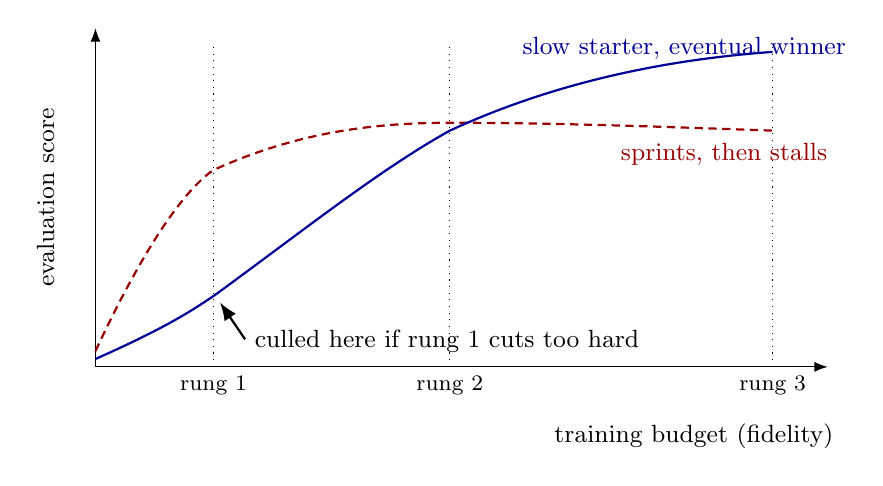
\begin{tikzpicture}[scale=1.0, font=\small]
\draw[-{Latex}] (0,0) -- (9.3,0);
\node[anchor=north] at (7.6,-0.6) {training budget (fidelity)};
\draw[-{Latex}] (0,0) -- (0,4.3);
\node[rotate=90, anchor=south] at (-0.4,2.15) {evaluation score};
% rung lines
\foreach \x/\l in {1.5/rung 1, 4.5/rung 2, 8.6/rung 3}
  \draw[dotted] (\x,0) node[below, font=\footnotesize] {\l} -- (\x,4.1);
% fast starter that stalls
\draw[thick, red!60!black, densely dashed]
  (0,0.2) .. controls (0.7,1.7) and (1.2,2.3) .. (1.5,2.5)
  .. controls (2.6,3.0) and (3.6,3.1) .. (4.5,3.1)
  .. controls (5.8,3.1) and (7.2,3.05) .. (8.6,3.0);
\node[red!60!black, anchor=west] at (6.55,2.7) {sprints, then stalls};
% slow starter that wins
\draw[thick, blue!60!black]
  (0,0.1) .. controls (0.9,0.5) and (1.2,0.7) .. (1.5,0.9)
  .. controls (2.6,1.7) and (3.6,2.5) .. (4.5,3.0)
  .. controls (5.8,3.6) and (7.2,3.9) .. (8.6,4.0);
\node[blue!60!black, anchor=west] at (5.3,4.05) {slow starter, eventual winner};
% cull marker at rung 1
\draw[-{Latex}, thick] (1.9,0.35) -- (1.58,0.82);
\node[anchor=west, align=left] at (1.9,0.32) {culled here if rung 1 cuts too hard};
\end{tikzpicture}
\caption{The multi-fidelity hazard (schematic). At rung 1 (the first of
the budget checkpoints that this chapter's ladders call rungs) the aggressive
configuration leads and the eventual winner trails; their curves cross
between rungs 1 and 2. Every method in this chapter is a different answer
to the question ``how hard may we cut on early evidence, given that curves
cross?'', and the honest answer starts with measuring how often they cross
on the workload at hand.}
\label{fig:curves}
\end{figure}

\section{Successive halving: the arithmetic of courage}

Successive halving spends a budget on many cheap looks and a few expensive
ones \citep{jamieson2016successive}. Fix a reduction factor $\eta$
(usually 3). Give every starter a small budget $r$; keep the best $1/\eta$
fraction and give each survivor $\eta$ times more budget; repeat. The
rounds of this ladder are called \emph{rungs}, and the race ends when
one rung remains. Rung sizes shrink by $\eta$ while per-trial budgets grow by
$\eta$, so every rung costs about the same, and there are about
$\log_\eta n$ rungs of them.

The numbers deserve one concrete pass, because the savings are the whole
argument. Take the running example with $n = 81$ starting configurations,
$\eta = 3$, and an initial budget of $r$ = 1 unit, where 81 units is a
full training run (so one unit is just under two million environment
steps). The rungs then look like this:
81 trials at 1 unit each (cost 81), the best 27 continue to 3 units
(cost 81), the best 9 continue to 9 units (cost 81), the best 3 continue
to 27 units (cost 81), and the single survivor runs to the full 81 units
(cost 81). Total: 405 units, about five full-length runs, to triage 81
configurations. Evaluating all 81 at full length would have cost
$81 \times 81 = 6561$ units, a factor of sixteen more; even the standard
sixteen-full-runs budget of the RL study in
Chapter~\ref{sec:workloads} could not have screened a fifth as many
candidates at full fidelity. Figure~\ref{fig:sh} draws the resulting
shape: the budget is a rectangle of constant area per rung, spent mostly
on configurations that survived at least one cut.

\begin{figure}[t]
\centering
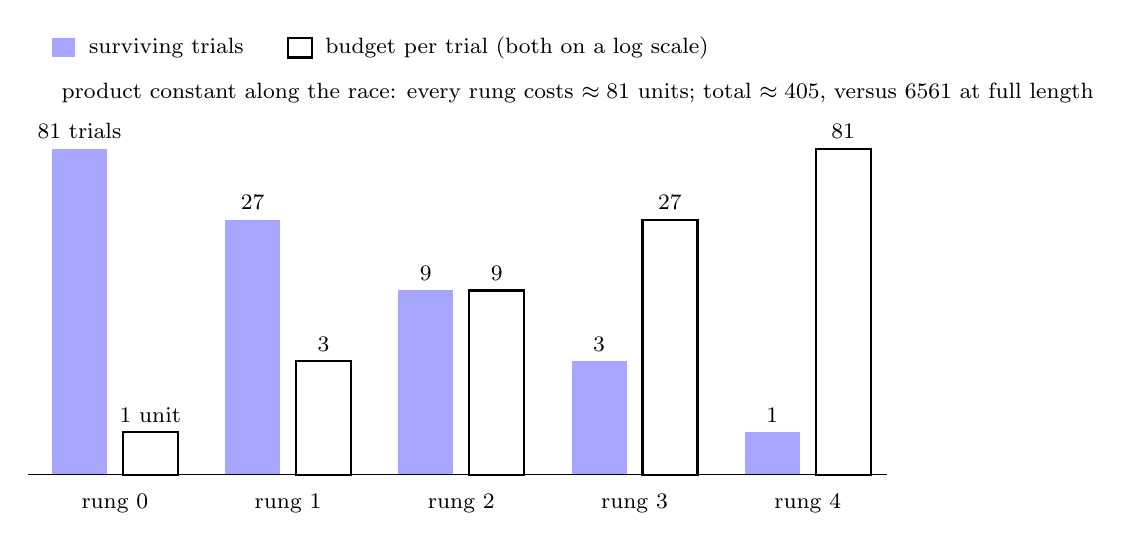
\begin{tikzpicture}[font=\small]
% paired bars per rung: filled = surviving trials, open = per-trial budget (log scale)
\foreach \rung/\ha/\hc/\la/\lc in {0/4.14/0.54/81 trials/1 unit, 1/3.24/1.44/27/3, 2/2.34/2.34/9/9, 3/1.44/3.24/3/27, 4/0.54/4.14/1/81} {
  \fill[blue!35] (2.2*\rung,0) rectangle (2.2*\rung+0.7,\ha);
  \draw[thick] (2.2*\rung+0.9,0) rectangle (2.2*\rung+1.6,\hc);
  \node[anchor=south, font=\footnotesize] at (2.2*\rung+0.35,\ha) {\la};
  \node[anchor=south, font=\footnotesize] at (2.2*\rung+1.25,\hc) {\lc};
  \node[anchor=north, font=\footnotesize] at (2.2*\rung+0.8,-0.12) {rung \rung};
}
\draw (-0.3,0) -- (10.6,0);
% legend
\fill[blue!35] (0.0,5.3) rectangle (0.3,5.55);
\node[anchor=west, font=\footnotesize] at (0.35,5.42) {surviving trials};
\draw[thick] (3.0,5.3) rectangle (3.3,5.55);
\node[anchor=west, font=\footnotesize] at (3.35,5.42) {budget per trial (both on a log scale)};
\node[anchor=west, font=\footnotesize, align=left] at (0.0,4.85)
  {product constant along the race: every rung costs $\approx 81$ units; total $\approx 405$, versus $6561$ at full length};
\end{tikzpicture}
\caption{One successive-halving bracket on the running example
($n = 81$, $\eta = 3$). At each rung the surviving trials shrink by the
factor the per-trial budget grows by, so the two staircases mirror each
other and every rung costs the same 81 units: the whole screen of 81
configurations costs about five full-length runs. The scheme's entire
risk is concentrated in the cuts between rungs, where
Figure~\ref{fig:curves}'s crossing curves get judged early.}
\label{fig:sh}
\end{figure}

The rub is the choice of the starting budget $r$: too small and slow
starters die unfairly (the hazard of Figure~\ref{fig:curves} at its
sharpest), too large and the savings evaporate. Hyperband declines to
choose. It runs several successive-halving brackets, from aggressive
(many configurations, tiny initial budget) to conservative (few
configurations, nearly full initial budget), giving each bracket the
same total budget, and provably loses only a logarithmic factor to the
best bracket in hindsight \citep{li2018hyperband}. Continuing the
numbers above ($\eta = 3$, full budget 81 units), the five brackets
start 81 trials at 1 unit, 34 at 3, 15 at 9, 8 at 27, and 5 at the full
81, each bracket then halving as before; each costs about 405 units, so
the whole portfolio costs about 2025 units, twenty-five full-run
equivalents to hedge every plausible answer to ``how early is too early
to judge.'' On a workload where early rankings are honest, the
aggressive brackets deliver; on one where curves cross late, the
conservative brackets are the insurance policy that was bought in
advance.

\section{The asynchronous turn}

Both methods as stated are synchronous: a rung must fully finish before
promotions happen, so a single straggler idles the fleet. With hundreds
of workers this is not a corner case; it is the steady state.

ASHA,
the asynchronous successive halving algorithm,
removes the barrier \citep{li2020asha}. Whenever a worker frees up, look
at the topmost rung that has a promotable trial: promote any
configuration that is in the top $1/\eta$ of the results recorded so far
at its rung; otherwise start a fresh configuration at the bottom rung.
Concretely: with $\eta = 3$, the moment the fourth result lands on a
rung, its best member is in the top third of four and can be promoted
immediately, without waiting for trials five through eighty-one.

Early
promotions are sometimes wrong (judged against a rung that was not full
yet), and ASHA accepts this deliberately: the authors' experiments show
the aggressiveness costs little in final quality while keeping hundreds
of workers busy, and ASHA has become the standard early-stopping
scheduler in distributed tuners, including Ray Tune's implementation.
The design lesson generalizes and will return in
Chapter~\ref{sec:population}: at scale, a slightly worse decision now
beats a slightly better decision after a barrier.

Two refinements are worth knowing. PASHA grows the maximum fidelity
progressively and stops growing it once the ranking of survivors
stabilizes, saving the top-rung budget when the decision is already
clear \citep{bohdal2023pasha}. The median stopping rule, older and
model-free, simply kills any trial whose running average falls below the
median of completed trials at the same step \citep{golovin2017vizier};
it composes with any searcher and is the cheapest insurance policy we
can offer users.

\section{Putting the model back: BOHB, DEHB, and racing}

Bandit schedulers decide when to stop but sample new configurations
blindly: the bottom rung of every bracket above was filled by random
search. After Chapter~\ref{sec:bayesian}, the obvious repair is to let a
model choose what enters the race. BOHB, Bayesian optimization plus
Hyperband as its name says, runs Hyperband's brackets but
draws new configurations from a TPE fit at the highest fidelity that has
enough observations, so the racing machinery keeps its budget arithmetic
while the entrants improve over time \citep{falkner2018bohb}. DEHB
replaces the sampler with differential evolution
(Chapter~\ref{sec:modelfree}): a subpopulation evolves at each rung, and
information flows across fidelities through the evolutionary operations
themselves, survivors of cheap rungs seeding the recombination that
proposes candidates for expensive ones, rather than through a fitted
density model \citep{awad2021dehb}.

DEHB deserves particular attention from us: in the controlled comparison
of \citet{eimer2023hyperparameters} across PPO and two other standard
RL algorithms (SAC and DQN) on eleven
environments, DEHB was the most consistent tuner at budgets of ten to
sixty-four full training runs, matching or beating hand tuning, random
search, and the population methods, all at negligible optimizer
overhead. That is precisely the budget regime our routine RL studies
live in, and Chapter~\ref{sec:workloads} builds the recommendation on
it. SMAC3 reaches a similar design point from the BO side, pairing its
random forest surrogate with successive-halving style racing of
incumbents \citep{lindauer2022smac3}.

\section{Modeling the learning curve itself}

Rung-based methods compare trials only at matching fidelities and throw
away the shape of the curve between rungs; in Figure~\ref{fig:curves},
the information that the blue curve was still rising steeply at rung 1
while the red curve had flattened is exactly what the rung comparison
discards. Learning-curve methods keep it. They model the whole
trajectory and ask a sharper question: given everything observed so far,
which paused trial (or which new one) should receive the next slice of
budget? Figure~\ref{fig:freezethaw} shows the decision problem: from a
partial curve, extrapolate a distribution over its continuation, and
weigh thawing the promising-but-uncertain run against extending the
solid-but-plateauing one.

\begin{figure}[t]
\centering
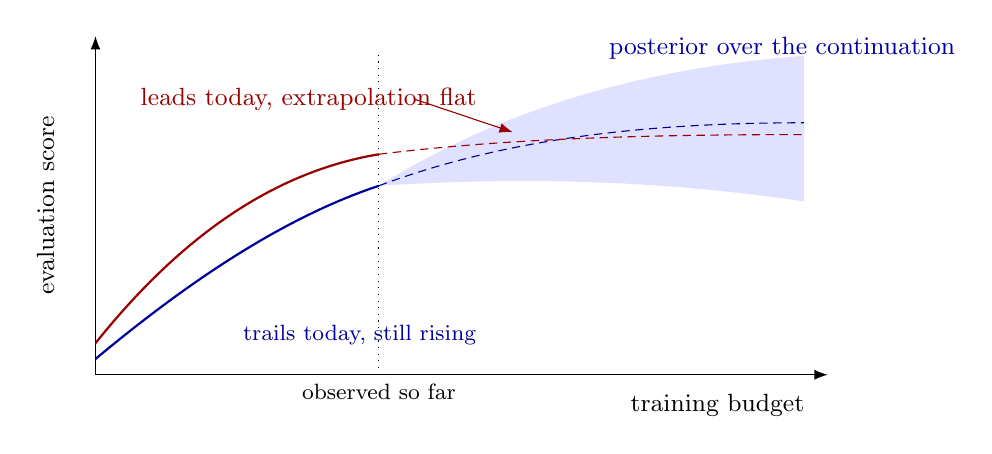
\begin{tikzpicture}[scale=1.0, font=\small]
\draw[-{Latex}] (0,0) -- (9.3,0);
\node[anchor=north] at (7.9,-0.12) {training budget};
\draw[-{Latex}] (0,0) -- (0,4.3);
\node[rotate=90, anchor=south] at (-0.4,2.15) {evaluation score};
\draw[dotted] (3.6,0) node[below, font=\footnotesize] {observed so far} -- (3.6,4.1);
% observed curve
\draw[thick, blue!60!black]
  (0,0.2) .. controls (1.2,1.2) and (2.4,2.0) .. (3.6,2.4);
% extrapolation fan
\fill[blue!12]
  (3.6,2.4) .. controls (5.2,3.4) and (7.0,3.9) .. (9.0,4.05)
  -- (9.0,2.2) .. controls (7.0,2.5) and (5.2,2.5) .. (3.6,2.4) -- cycle;
\draw[blue!60!black, densely dashed]
  (3.6,2.4) .. controls (5.2,3.0) and (7.0,3.2) .. (9.0,3.2);
\node[blue!60!black, anchor=west, align=left] at (6.4,4.15) {posterior over the continuation};
% competitor: paused flat curve
\draw[thick, red!60!black]
  (0,0.4) .. controls (1.2,1.9) and (2.4,2.6) .. (3.6,2.8);
\draw[red!60!black, densely dashed]
  (3.6,2.8) .. controls (5.2,3.0) and (7.0,3.05) .. (9.0,3.05);
\node[red!60!black, anchor=west] at (0.45,3.5) {leads today, extrapolation flat};
\draw[red!60!black, -{Latex}] (4.05,3.5) -- (5.3,3.08);
\node[blue!60!black, anchor=west, font=\footnotesize] at (1.75,0.5) {trails today, still rising};
\end{tikzpicture}
\caption{The freeze-thaw decision (schematic). Both trials are paused at
the dotted line. The red trial leads today but its extrapolation is
flat; the blue trial trails with a rising curve and a wide posterior
over where it ends up. A learning-curve method allocates the next budget
slice by comparing these posteriors, information that rung-based
promotion never sees.}
\label{fig:freezethaw}
\end{figure}

The idea goes back to freeze-thaw Bayesian optimization
\citep{swersky2014freezethaw}, which kept a basket of paused runs
(freeze a run to pause it, thaw it to resume) and
used a GP with an exponential-decay kernel over training curves to
decide which to thaw. Every modern instance keeps that decision
structure and changes one component, the curve model, and the choice
matters more than it sounds, because the curve model is refit inside
the decision loop: whatever it costs is paid again at every
allocation decision.

DyHPO makes the curve model a deep-kernel GP over the triple of
configuration, budget, and partial curve, and greedily advances
whichever candidate has the best expected improvement one step ahead
\citep{wistuba2022dyhpo}. The price follows from
Chapter~\ref{sec:bayesian}: GP fitting is cubic in the number of
observations, and a curve observed at every epoch multiplies
observations quickly, so the surrogate's bill grows with exactly the
data that makes it useful.

DPL swaps the GP for an ensemble of power-law extrapolations,
motivated by the empirical regularity that neural training curves
follow approximate power laws; the spread of the ensemble supplies
the uncertainty that the acquisition needs \citep{kadra2023dpl}. The
model is lighter than a deep-kernel GP, but the ensemble is still
refit inside the loop.

ifBO (in-context freeze-thaw BO) removes the in-loop fitting entirely.
Its curve model is a prior-fitted network: a transformer (the neural
architecture behind modern language models) pre-trained once on
synthetic learning curves, which then performs Bayesian curve
extrapolation
in-context, in a single forward pass, one to two orders of magnitude
faster than fitting DyHPO's deep GP or DPL's ensembles inside the
loop. The acquisition paired with it randomizes its lookahead horizon
and improvement threshold \citep{rakotoarison2024ifbo}.
Chapter~\ref{sec:transfer} explains what a prior-fitted network is
and why ``pre-trained once'' is the phrase that changes the
economics.

The evidence and the price, briefly, before the evidence section
weighs both. On the multi-fidelity benchmarks used in those papers,
the learning-curve methods dominate rung-based baselines when curves
are informative. The price is operational: the tuner must be able to
pause, checkpoint, and resume trials at fine granularity, which is
exactly the machinery that Ray Tune trials and RLlib checkpoints
already expose.

The honest summary for our roadmap: ASHA plus a good searcher is the
sturdy default that captures most of the savings; DEHB is the
evidence-backed choice at small RL budgets; learning-curve methods are
the frontier worth one focused implementation
(Chapter~\ref{sec:roadmap}) once the pause and resume plumbing is
solid, with ifBO the most attractive because the surrogate arrives
pre-trained rather than being refit inside the loop.

\section{The evidence, and how much of it is arithmetic}
\label{sec:mf-evidence}

Those verdicts lean on four different grades of support, and the
grades are worth keeping separate because each properly carries a
different weight of decision: arithmetic, which requires no trust in
anyone; theory, which is genuine but conditional; the method authors'
own benchmarks; and a single independent study on live training runs.
Section~\ref{sec:bo-evidence} argued that evidence should be weighed
by how it was produced. Applied here, that principle sorts the
chapter's claims cleanly.

The arithmetic came first, and it is the part that cannot be argued
with. The 405-versus-6561 comparison under Figure~\ref{fig:sh} is not
an experimental finding; given the rung geometry, the factor of
sixteen follows by multiplication, and no benchmark can add to it or
take it away. What multiplication cannot supply is a promise that the
cheap rungs \emph{select} well, and the theory is candid about the
same limit. The successive-halving guarantee is of a deliberately
modest kind, bounding identification error under assumptions on how
fast each training curve settles toward its final value, and
Hyperband's theorem promises performance within a logarithmic factor
of the best bracket in hindsight, not good performance outright
\citep{jamieson2016successive, li2018hyperband}. Neither theorem knows
whether the curves of our workloads settle quickly enough for early
rankings to be trusted. That is a property of the workload, not of
the algorithm, which is why the rank-correlation pilot suggested at
the chapter's opening is the one empirical measurement the whole
apparatus genuinely needs.

ASHA's evidence is of another kind again, and the paper it comes from
announces what kind: this is a systems paper, written around the
production tuning service its authors were building, and its central
claims are operational \citep{li2020asha}.

The distributed
experiments compare ASHA against synchronous successive halving,
BOHB, and PBT (the population method Chapter~\ref{sec:population}
teaches) with twenty-five workers on two image-classification tuning
tasks (CIFAR-10),
five runs of each method, and the finding is the one the mechanism
predicts: on the task where training times vary across
configurations, the synchronous methods idle at their barriers and
ASHA pulls cleanly ahead, while on the task where they do not, the
schedulers roughly agree, ASHA reaching a good configuration about
1.5 times sooner and BOHB ending slightly ahead on final quality. On
two architecture search spaces with sixteen workers, ASHA reached a
below-ten-percent test error roughly twice as fast as synchronous
halving and BOHB and ended slightly ahead on average. The
demonstration that justifies the word ``massive'' ran five hundred
workers for weeks on a recurrent language-model space.

All of this is the authors' own
arena, and the selection-bias caution of
Section~\ref{sec:bo-evidence} applies; two things temper it here.
The claim under test is throughput rather than statistical
cleverness, so a skeptic can audit the mechanism (promote now
against the top third observed so far, never wait) instead of
trusting a tuned baseline. And the operational half of the claim has
been replicated the way operational claims are: ASHA is the standard
early-stopping scheduler in the distributed tuners we audited
(Chapter~\ref{sec:libraries}), adopted by teams with no stake in the
paper.

DEHB's support arrives in two installments, and the order matters.
The authors' own paper is a breadth exercise: toy functions,
surrogate and tabular benchmarks, and thirteen tabular
architecture-search benchmarks, against random search, TPE, GP-based
BO, SMAC, Hyperband, and BOHB, with headline speedups of up to a
factor of a thousand over random search and thirty-two over BOHB
\citep{awad2021dehb, falkner2018bohb}.

Two features of that design
are worth noticing before the numbers settle in. Nearly all of the
benchmarks are tabular or surrogate, meaning the training runs were
paid for once, offline, and the tuners replay or interpolate them,
with optimizer overhead excluded from the cost axis by construction
(a choice that, if anything, understates DEHB's cheapness relative
to the model-based methods). And the paper reports its own boundary
case plainly: on NAS-Bench-101, where cheap-fidelity and
full-fidelity results correlate weakly, DEHB behaves like random
search early on, which is Figure~\ref{fig:curves}'s hazard surfacing
in the method's own results.

The second installment is the
independent one, and it is what this chapter's verdict actually
stands on: the budget-matched, seed-split RL study of
\citet{eimer2023hyperparameters}, run on live training at ten to
sixty-four full runs, whose design is laid out in
Section~\ref{sec:pop-evidence}, found DEHB the most consistent tuner
in exactly the regime our routine studies inhabit. The authors'
benchmarks nominate the method; the independent live study is what
promotes it.

The learning-curve methods sit at the far end of the scale. Their
support is the authors' own, on multi-fidelity benchmark suites
built for the purpose, with no independent budget-matched test on
live RL training at our budgets yet \citep{wistuba2022dyhpo,
kadra2023dpl, rakotoarison2024ifbo}. That is not a criticism; it is
where every young line of methods starts, and it is precisely the
evidentiary grade at which a sensible product buys an option rather
than installs a default. The chapter's decisions read directly off
this scale. The always-on default rests on arithmetic, a measurable
hazard, and an operational record; the small-budget RL pick rests on
one independent controlled study; the frontier bet rests on
promising author-run comparisons, and is gated accordingly.

\section{The default, argued from four angles}
\label{sec:mf-angles}

The chapter's verdict is that early stopping is not optional
equipment: ASHA with the median rule as the always-on default, DEHB
where a study is a few dozen full runs of RL, the learning-curve
line as a gated bet. As in Chapter~\ref{sec:bayesian}, four
independent lines of argument arrive at the same place, and a reader
should demand that they agree.

From arithmetic: the savings factor is an identity, not an estimate.
Sixteenfold on the worked bracket, an order of magnitude in general,
and the only empirical quantity the identity leans on, whether early
rankings predict late ones, is measurable on the workload at hand
for the price of a pilot. A default whose upside is multiplication
and whose risk is one measurable number stands on firmer ground than
anything else in this document.

From evidence: the sources agree at the boundary. The theory
conditions its guarantees on curves settling; DEHB's own benchmarks
degrade toward random search exactly where fidelities decorrelate;
the one independent live-RL study finds the rung family most
consistent at exactly the budgets where the arithmetic bites
hardest. Three kinds of source, none sharing authors, point at the
same governing variable, the trustworthiness of cheap evaluations,
and that is the variable our pilot measures and our defaults
respect.

From operations: ASHA and the median rule ask one thing of training
code, that it report a metric as it goes, and nothing at all of the
searcher, so they compose with every method of
Chapters~\ref{sec:modelfree} and \ref{sec:bayesian} rather than
competing with them. The asynchronous design is what lets a schedule
survive contact with a shared cluster, where stragglers are the
steady state and every barrier converts one slow trial into
fleet-wide idleness. The learning-curve methods' operational price,
pause and resume at fine granularity, is real, which is why their
entry is gated on plumbing the roadmap builds anyway for the
population methods of Chapter~\ref{sec:population}.

From decision theory: the two ways to be wrong cost differently.
Stopping too eagerly risks killing a slow starter, a bounded loss
that the rank-correlation pilot prices in advance and a conservative
bracket insures against; stopping too late, or not at all, pays the
full factor of sixteen with certainty. When one error is bounded,
diagnosable, and insurable and the other is certain and large, the
default must accept the first risk, which is exactly what an
aggressive-by-default, insurable-by-option scheduler does.

And the criterion that could overturn the verdict, stated in
advance: the validation suite of Chapter~\ref{sec:roadmap} races
ASHA plus a searcher against the same searcher at full fidelity on
the pinned tasks at matched total budgets, repeated across seeds; it
logs between-rung rank correlations on every study it touches, so
the crossing-curves hazard becomes a measured quantity of our
workloads rather than a literature anecdote; and DEHB is re-raced
against BO plus ASHA at sixteen to sixty-four runs on the pinned RL
task. If early stopping costs final quality on our workloads, the
default flips to conservative brackets, and the suite, not this
chapter, has the last word.

\begin{decisions}
\noindent\textbf{Decisions from this chapter.} Multi-fidelity is where
the money is saved, so every verdict here is really a claim about
compute bills.
\begin{itemize}[leftmargin=1.3em, itemsep=2pt]
\item \textbf{ASHA plus the median stopping rule} (include; days;
tier 0). The workhorse pair. Between them they capture the bulk of the
order-of-magnitude savings this chapter promises, compose with any
searcher, and ask almost nothing of the training code beyond reporting
a metric as it goes. If the package shipped only one scheduler, it
would be this one.
\item \textbf{Hyperband as a distinct feature} (exclude). Its
insurance-portfolio idea survives inside our defaults (run a
conservative bracket when curve crossing is suspected), but as a
product surface ASHA superseded it and no user-facing knob is worth
the confusion.
\item \textbf{BOHB} (exclude). The idea, model-guided entrants into
the race, lives on in our BO-plus-ASHA composition; the reference
implementation is formally unmaintained
(Chapter~\ref{sec:libraries}), and adopting it would import a dead
dependency for no capability we lack.
\item \textbf{DEHB, implemented against our interfaces} (include;
weeks; tier 3). The one scheduler-searcher hybrid with controlled RL
evidence behind it at exactly our routine budgets: most consistent
tuner at ten to sixty-four full runs across PPO, SAC, and DQN
\citep{eimer2023hyperparameters}. The upstream package is frozen, so
this is a reimplementation with the original as reference, not a
wrap.
\item \textbf{PASHA} (include as an ASHA option flag; small). Stops
paying for top-rung training once the ranking has stabilized; cheap
to add because it is a stopping condition, not a new scheduler.
\item \textbf{Learning-curve scheduling, specifically ifBO} (include;
tier 3 bet; weeks, gated on pause/resume plumbing). The only entry
that uses the shape of the curve between rungs
(Figure~\ref{fig:freezethaw}), and the variant whose surrogate is
pre-trained once rather than refit inside our loop, which is what
makes its overhead tolerable \citep{rakotoarison2024ifbo}. DyHPO and
DPL taught the field the idea; we adopt the version that ships.
\end{itemize}
\end{decisions}

\section{What would overturn these verdicts}

ASHA's tier-0 status depends on V06: if early stopping cannot match
full-fidelity final quality at a fraction of compute on our tasks,
or if rung-final rank correlations on real studies fall consistently
below the crossing-curves threshold, the scheduler is demoted and
budgets revert to full runs. DEHB's small-budget RL verdict is tied
to V07; if it loses to BO+ASHA at matched sixteen-run budget, it is
excluded and the register updated. The ifBO curve model's gating
(V15) is the designed check: if it does not match ASHA on public
suites before integration, the build is canceled and the tier-2 slot
reallocated. BOHB's explicit exclusion is reopened if the Optuna
wrap becomes negligible-cost and a colleague requests it with a use
case the box did not consider.

\chapter{Tuning while training: the population-based family}
\label{sec:population}

Everything so far searches for one fixed configuration, and the second bend
of Section~\ref{sec:formal} has been waiting patiently: in the running
example, the best learning rate at step zero is not the best learning rate
at step 100 million, because the agent's own improving policy keeps changing
the data it trains on. Population-based training (PBT) is the family that
takes this seriously. It searches for a \emph{schedule}, and it does so
inside a single training run, which is why it occupies a special place in
reinforcement learning, where the optimal learning rate, entropy bonus, or
batch size at the start of training is rarely optimal at the end.

\section{PBT: exploit, explore, inherit}

PBT trains a population of $B$ agents in parallel, each with its own
hyperparameters and its own network weights \citep{jaderberg2017pbt}. Every
$t_{\mathrm{ready}}$ steps, two operations run
(Figure~\ref{fig:pbt}). In the \emph{exploit} step, each agent in the
bottom fraction of the population (by current evaluation score) abandons
its own progress: it copies both the network weights and the
hyperparameters of an agent sampled from the top fraction, a rule known as
truncation selection. In the \emph{explore} step, the copied
hyperparameters are perturbed, in the original paper by random
multiplicative jitter or resampling from the prior. Training then
continues from the copied weights. Because weights are inherited rather
than restarted, the population performs a single collective training run
whose hyperparameters adapt on the fly, and the lineage of the final best
agent traces out a hyperparameter schedule that no pointwise tuner could
have expressed: in Figure~\ref{fig:pbt}, the winning agent's history runs
through two exploit events and three different learning rates, and that
whole trajectory, not its endpoint, is the method's output.

The figure repays one slow read-through, event by event, because every
later argument about this family refers back to it. Four agents train
in parallel, each with its own learning rate. At the first ready event,
the population is ranked by current evaluated return; the bottom agent
(lane two) is culled, receives a byte-for-byte copy of the top agent's
network weights and hyperparameters, has those hyperparameters
perturbed, and resumes training from the copied weights rather than
from scratch.

Between the first and second ready events, four
\emph{different} hyperparameter settings are being evaluated while
four networks make training progress; no compute is spent on rehearsal
runs that will be thrown away, which is the family's core economy.

At
the second ready event the same surgery repeats on the new laggard.
The winning agent's bold lineage, read left to right, is a sequence of
(weights inherited, hyperparameters revised) segments: a learning-rate
\emph{schedule} discovered by selection, with no schedule ever
specified. That is the object no method in the previous chapters can
produce, and it is also, as the next paragraphs show, the source of
the family's characteristic failures.

\begin{figure}[t]
\centering
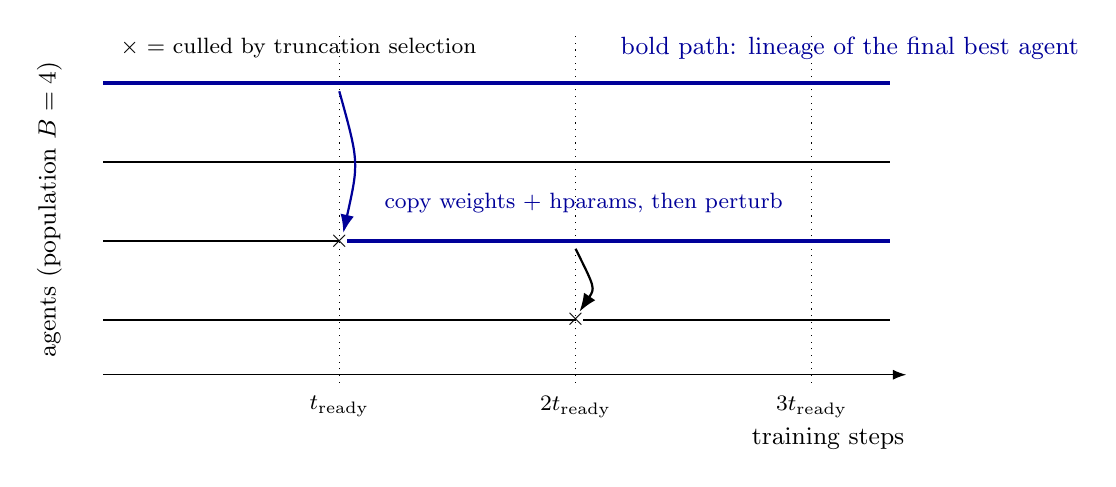
\begin{tikzpicture}[scale=1.0, font=\small]
% axes
\draw[-{Latex}] (0,0) -- (10.2,0);
\node[anchor=north east] at (10.3,-0.55) {training steps};
\node[rotate=90, anchor=south] at (-0.4,2.1) {agents (population $B=4$)};
% ready-event lines
\foreach \x in {3.0,6.0,9.0} \draw[dotted] (\x,-0.1) -- (\x,4.3);
\node[font=\footnotesize, anchor=north] at (3.0,-0.15) {$t_{\mathrm{ready}}$};
\node[font=\footnotesize, anchor=north] at (6.0,-0.15) {$2t_{\mathrm{ready}}$};
\node[font=\footnotesize, anchor=north] at (9.0,-0.15) {$3t_{\mathrm{ready}}$};
% agent lanes at y = 0.7, 1.7, 2.7, 3.7
% agent 4 (top lane): strong performer, survives; lineage bold
\draw[line width=1.5pt, blue!60!black] (0,3.7) -- (3.0,3.7);
\draw[line width=1.5pt, blue!60!black] (3.0,3.7) -- (6.0,3.7);
\draw[line width=1.5pt, blue!60!black] (6.0,3.7) -- (9.0,3.7) -- (10.0,3.7);
% agent 3
\draw[thick] (0,2.7) -- (3.0,2.7);
\draw[thick] (3.0,2.7) -- (6.0,2.7);
\draw[thick] (6.0,2.7) -- (10.0,2.7);
% agent 2: culled at t_ready, copies agent 4
\draw[thick] (0,1.7) -- (3.0,1.7);
\node at (3.0,1.7) {$\times$};
\draw[-{Latex}, thick, blue!60!black] (3.0,3.6) .. controls (3.25,2.7) .. (3.05,1.8);
\draw[line width=1.5pt, blue!60!black] (3.1,1.7) -- (6.0,1.7) -- (9.0,1.7);
\draw[line width=1.5pt, blue!60!black] (9.0,1.7) -- (10.0,1.7);
\node[blue!60!black, font=\footnotesize, anchor=west] at (3.45,2.18) {copy weights + hparams, then perturb};
% agent 1: culled at 2t_ready, copies agent 2's line
\draw[thick] (0,0.7) -- (6.0,0.7);
\node at (6.0,0.7) {$\times$};
\draw[-{Latex}, thick] (6.0,1.6) .. controls (6.25,1.1) .. (6.05,0.8);
\draw[thick] (6.1,0.7) -- (10.0,0.7);
% winner label
\node[blue!60!black, anchor=west, align=left, font=\small] at (6.45,4.15)
  {bold path: lineage of the final best agent};
\node[anchor=west, font=\footnotesize] at (0.1,4.15) {$\times$ = culled by truncation selection};
\end{tikzpicture}
\caption{One PBT run (schematic, $B = 4$). At each ready event the bottom
agents are culled and restart from copies of top agents' weights and
hyperparameters, perturbed before training resumes. The bold lineage is
the method's real product: a hyperparameter \emph{schedule} that switched
values twice mid-run, expressed by no pointwise method in this document.}
\label{fig:pbt}
\end{figure}

Two ablations in the original paper pin down where the value lives, and
they are the reason we drew the lineage rather than the final point.
Rerunning training from scratch with the final PBT-found hyperparameters
underperformed PBT itself, so the schedule rather than the endpoint
carries the gain; and populations of around twenty gave consistent
improvements with diminishing returns beyond. The cost structure is
equally distinctive: one PBT run costs $B$ training runs of wall-clock
length one, fully parallel, rather than a long sequence of trials. When a
project has $B$ machines and one calendar week, that shape is not a detail;
it is the argument.

Two failure modes matter as much as the mechanism. First, PBT is greedy:
truncation selection optimizes the \emph{current} score, and
Figure~\ref{fig:curves} already showed what current scores do to
configurations that invest now to pay off later. A small learning rate or
a heavy regularizer is exactly the blue curve of that figure, and
truncation selection is the cull arrow. FIRE-PBT (faster improvement
rate PBT) counters this by scoring
sub-populations on their rate of improvement rather than their level, and
the size of the greediness cost is worth quoting: on ImageNet, the
learning-rate schedule found by greedy PBT reached 71.7 percent top-1
accuracy where FIRE-PBT reached 76.5, essentially matching the hand-tuned
schedule at 76.6 \citep{dalibard2021firepbt}.

Second, with the modest
populations we can afford (the experiments below use $B = 8$), copying
weights across the population collapses diversity in weight space: after
a few exploit events, every agent descends from the same early winner,
and the search degenerates into local perturbation around one basin.
\citet{wan2022bgpbt} observed both effects directly: on four of their
seven Brax tasks, plain random search matched or beat both PBT and PB2 at
the same compute, which they attribute to exactly this
premature-convergence behavior.

\section{PB2: replacing random perturbation with a bandit}

The explore step is where PBT wastes its evidence: jitter treats the
population's accumulated experience as worthless. PB2 repairs it with the
machinery of Chapter~\ref{sec:bayesian} \citep{parkerholder2020pb2}. PB2
records every observed (hyperparameters, training-progress) increment
across the population and fits a Gaussian process whose kernel includes a
time coordinate, so that old evidence decays: an observation from early
training informs, but does not dictate, beliefs about what works now.

When an agent needs new hyperparameters after an exploit event, PB2
chooses them by maximizing a UCB acquisition, the rule of
\eqref{eq:ucb} applied to this time-varying surrogate: for the increment
model $\hat{f}_t$ with posterior mean $\mu_t$ and spread $s_t$, pick
\begin{equation}
\config_{\mathrm{new}}
\in \arg\max_{\config \in \cspace}\;
\mu_t(\config) + \beta_t^{1/2}\, s_t(\config),
\label{eq:pb2}
\end{equation}
maximization now because the increment is a reward. Members of the batch
whose outcomes are still pending are handled by updating the posterior
variance as if their results were already in (the fantasy device of
Section~\ref{sec:acquisition}), so the whole population can be proposed
at once.

The quantity modeled is deliberately the \emph{increment} of
performance over one interval rather than its level, which is what makes
the bandit framing clean: total performance is the sum of increments, so
maximizing final performance equals minimizing cumulative regret over
increments, and the authors prove a sublinear-regret bound for the
resulting time-varying GP bandit. Sublinear regret has a plain reading:
the average quality gap between the bandit's choices and the best
choices available at each moment goes to zero as training proceeds.

A follow-up, PB2-Mix, adds categorical hyperparameters through a
hierarchical explore step: a time-varying adversarial bandit picks the
categories, then the GP picks the continuous coordinates conditioned on
that choice, with the regret guarantee extended to the mixed space
\citep{parkerholder2021pb2mix}.

The empirical promise is sample
efficiency at small population sizes, but two independent observations
temper it: the BG-PBT ablations show a plain GP surrogate limits how much
of the space PB2 can cover \citep{wan2022bgpbt}, and in the
budget-constrained study of \citet{eimer2023hyperparameters}, PB2's tuned
configurations changed at most once over a run (so the schedule
advantage, the entire point of Figure~\ref{fig:pbt}, went unused) and its
incumbents transferred poorly to fresh seeds.

\section{BG-PBT: trust-region BO plus generational architecture search}

BG-PBT, the method we were specifically asked to evaluate, upgrades both
halves of PBT and adds architecture search \citep{wan2022bgpbt}. We read
the paper in full; what follows is its actual content rather than its
abstract. Readers will recognize every ingredient: the search space is
the running example's, the searcher is Section~\ref{sec:highdim}'s
trust-region machinery, and the schedule-versus-point distinction is
Figure~\ref{fig:pbt}'s.

The search space is the full RL configuration. For their PPO-on-Brax
experiments this means nine training hyperparameters (learning rate,
discount, entropy coefficient, unroll length, reward scaling, batch size,
update epochs, GAE $\lambda$, clipping $\epsilon$) plus six architecture
parameters (width, depth, and a spectral-normalization flag for policy
and value networks separately), the 15-dimensional mixed space of
continuous, ordinal, and categorical coordinates that
Section~\ref{sec:running} adopted as our running example.

The explore
step becomes a high-dimensional mixed-space BO agent built on
Casmopolitan \citep{wan2021casmopolitan}: kernels tailored to each
coordinate type (their extension treats ordinals as ordered rather than
categorical, with measurable gains in their ablation), acquisition
optimization that interleaves local search over discrete coordinates
with gradient steps over continuous ones, and trust regions around the
current best configuration exactly as in Figure~\ref{fig:turbo},
expanding on successes, shrinking on failures, and triggering a restart
with a fresh surrogate when they collapse, guided by a UCB rule on an
auxiliary global GP. Restarts matter more here than in the static
setting of Section~\ref{sec:highdim}: in a time-varying problem they are
what stops the surrogate from anchoring on stale evidence.

The authors
extend the regret guarantee of PB2 to this trust-region, mixed-space,
time-varying setting (their Theorem 3.1), with the usual caveat that
the guarantee covers the version without architecture transfer.

Architecture search enters through \emph{generations}, and the device
that makes it affordable is distillation
(Figure~\ref{fig:generations}). Within a generation, architectures are
fixed per agent; truncation selection copies weights \emph{and
architecture}, so poor architectures are squeezed out of the population,
and the BO agent conditions its hyperparameter suggestions on the
architecture coordinates as context. When the population's evaluated
return stagnates past a patience threshold, a new generation begins: a
fresh set of architectures is proposed (by random search plus successive
halving over the architecture subspace, later informed by a BO model fit
to the best score each architecture achieved), and the new agents are
trained initially by on-policy distillation from the best agent of the
outgoing generation, with a joint loss that anneals from imitation
(value regression plus a KL term to the teacher policy) into the plain
RL objective. Distillation is what makes changing architecture mid-run
affordable: the new network does not start from zero, it starts from an
imitation of the best agent so far.

\begin{figure}[t]
\centering
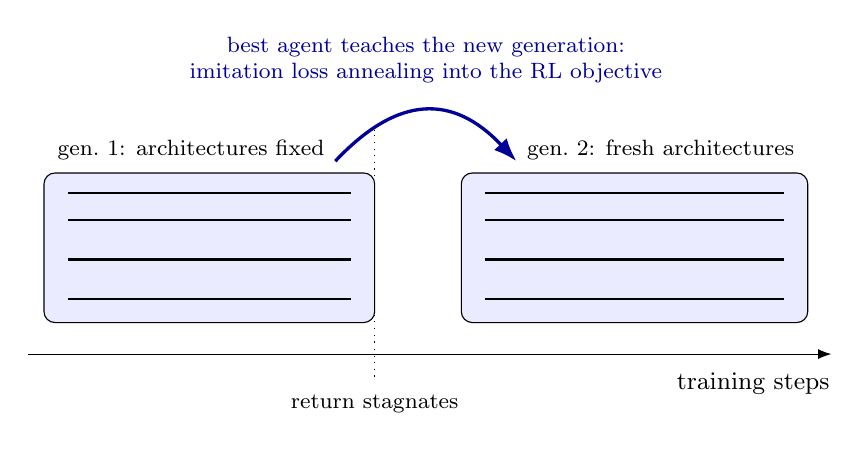
\begin{tikzpicture}[scale=1.0, font=\small]
\draw[-{Latex}] (0,0) -- (10.2,0);
\node[anchor=north east] at (10.3,-0.12) {training steps};
% generation 1 block
\draw[rounded corners, fill=blue!8] (0.2,0.4) rectangle (4.4,2.3);
\node[anchor=south west, font=\footnotesize] at (0.25,2.34) {gen.\ 1: architectures fixed};
\foreach \y in {0.7,1.2,1.7,2.05} \draw[thick] (0.5,\y) -- (4.1,\y);
% stagnation marker
\draw[dotted] (4.4,0.15) -- (4.4,2.85);
\draw[dotted] (4.4,0.15) -- (4.4,-0.35);
\node[anchor=north, font=\footnotesize] at (4.4,-0.4) {return stagnates};
% distillation arrow over the top
\draw[-{Latex}, very thick, blue!60!black] (3.9,2.45) .. controls (4.7,3.3) and (5.4,3.3) .. (6.2,2.45);
\node[blue!60!black, font=\footnotesize, anchor=south, align=center] at (5.05,3.32)
  {best agent teaches the new generation:\\imitation loss annealing into the RL objective};
% generation 2 block
\draw[rounded corners, fill=blue!8] (5.5,0.4) rectangle (9.9,2.3);
\node[anchor=south east, font=\footnotesize] at (9.85,2.34) {gen.\ 2: fresh architectures};
\foreach \y in {0.7,1.2,1.7,2.05} \draw[thick] (5.8,\y) -- (9.6,\y);
\end{tikzpicture}
\caption{BG-PBT's generational structure (schematic). Hyperparameters
adapt continuously inside a generation via the trust-region BO explore
step; architectures change only at generation boundaries, where new
networks are warm-started by distilling the outgoing best agent rather
than training from scratch. Distillation is the piece that makes
mid-run architecture change affordable.}
\label{fig:generations}
\end{figure}

The reported results, on seven Brax environments with population size 8
and 150M environment steps: BG-PBT reaches the best mean return on five
of seven tasks against tuned PPO, random search, PBT, and PB2, with the
remaining two split; against a sequential SMAC3 baseline given fifty
full runs (about six times the compute), BG-PBT still wins on four of
seven. The discovered schedules are interpretable and match folklore:
learning rates fall over training and batch sizes grow, without any
schedule having been specified. The paper's own limitations section
notes that on Humanoid the ablation without architecture search did
better, that generational transfer voids the theoretical guarantee, and
that the distillation hyperparameters are themselves fixed by hand. That
last item deserves a smile: the state of the art in hyperparameter
optimization contains, at its center, a handful of hand-tuned
hyperparameters. The regress has to stop somewhere, and knowing where it
stops is part of understanding the method.

\section{The two experiments this chapter's verdict rests on}
\label{sec:pop-evidence}

The verdict this chapter builds toward, build BG-PBT but confine the
whole population family to studies with real parallelism, rests on two
experiments. Section~\ref{sec:bo-evidence} argued that evidence should
be weighed by its design, not its abstract, so both designs are laid
out here in enough detail to be judged, and then the argument that
reconciles them is made explicitly, because at first reading they
appear to disagree.

The first experiment is the BG-PBT paper's own
\citep{wan2022bgpbt}. Seven Brax locomotion environments; PPO; a
population of eight agents; 150 million environment steps per run; the
fifteen-dimensional mixed search space of our running example, nine
training hyperparameters plus six architecture parameters. The
comparisons: PPO with tuned fixed hyperparameters, random search over
the same full space, original PBT, PB2, and, importantly, a
sequential SMAC3 baseline given fifty complete training runs, roughly
six times the compute of one population. The scoring is mean evaluated
return, and the headline results were quoted in the previous section:
best on five of seven tasks against the population-budget baselines,
still ahead on four of seven against the six-fold-compute sequential
baseline.

Three details of the design speak well of the authors.
Random search was run over the \emph{full} joint space rather than a
crippled subset, which is how the paper itself surfaced the
uncomfortable fact that random search matched or beat PBT and PB2 on
four of seven tasks. The ablations separate the contributions
(ordinal-aware kernels help; on Humanoid the version \emph{without}
architecture search did better). And the limitations section concedes
the points a referee would raise: the theory does not cover
generational transfer, and the distillation hyperparameters are set by
hand. A paper that reports where its own method loses earns more trust
than one that does not.

The second experiment is the controlled RL tuning study of
\citet{eimer2023hyperparameters}, from a different group with no
shared authors. Three algorithms (PPO, SAC, DQN) across eleven
environments, Brax tasks among them; tuners compared at matched
budgets of ten to sixty-four \emph{full training runs}, which is the
regime our routine studies actually inhabit; candidates evaluated on
several tuning seeds with final results reported on disjoint test
seeds the tuner never saw; and the tuners' own overhead measured
(minutes for most methods, about two hours for BG-PBT at the largest
budget, against days of trial compute).

The design's discipline is
the point: matched budgets stop a hungrier method from winning by
eating more, and the seed split stops a tuner from being rewarded for
overfitting luck. In this regime, DEHB was the most consistent tuner,
random search was respectable, and the population methods trailed:
BG-PBT sat behind DEHB and even random search at sixteen and
sixty-four runs, and PB2's tuned configurations changed at most once
per run, so the schedule advantage that justifies the family's
existence went unused. The authors note, fairly, that BG-PBT would
likely benefit from larger budgets.

Now the reconciliation, because a reader holding both results needs
it. The two experiments occupy different budget regimes. One
population run in the Wan design consumes eight parallel full-length
trainings, and its evolutionary machinery gets hundreds of exploit
events over 150 million steps; the Eimer design's entire budget is
ten to sixty-four full runs total, which starves a population method
of exactly the parallelism and step count its mechanism needs.

Where
the regimes overlap, the studies agree: both find random search over
the full space embarrassingly strong at modest budgets, and both find
plain PBT and PB2 fragile with small populations. So the apparent
contradiction is not one paper being wrong; it is one boundary seen
from both sides, and the boundary is the finding.

Below roughly eight
concurrent full-length workers or a few dozen full-run equivalents,
rung-based methods with a model (DEHB, or BO plus ASHA) are the
reliable choice; above it, with a schedule-shaped question, BG-PBT is
the strongest design published for that regime, on the evidence of
Brax locomotion at population sizes of eight and generous step
budgets, and its official implementation is available to build from. The package should enforce that boundary in
software rather than trust each user's optimism, and our validation
suite re-tests it on our own pinned tasks, since a boundary
established on Brax deserves a check before it governs a default.

\section{The family since 2022}

The line has stayed active, and the newer entries share one diagnosis:
PBT's remaining free parameter, the interval $t_{\mathrm{ready}}$
between evolution steps, is itself consequential and badly understood.
Evolve too often and agents are judged before their new hyperparameters
have had any effect; too rarely and the schedule cannot track the
drift it exists to track.

Multiple-frequencies PBT runs sub-populations
that evolve at different perturbation frequencies with an asymmetric
migration rule between them, reporting that vanilla PBT can fall behind
random search over long horizons, the same greediness disease FIRE-PBT
treats \citep{doulazmi2025mfpbt}. A 2026 preprint takes the opposite
tack for small populations, adjusting the interval through restarts
that reuse weights and re-seed hyperparameters by time-varying BO
\citep{chebykin2025ipbt}.

On the off-policy side (algorithms that learn from a stored
\emph{replay buffer} of past experience rather than only from the
freshest data), SEARL shares one replay
buffer across the whole population, so the meta-search rides on data the
population already paid for, a design worth remembering for our
off-policy RLlib work \citep{franke2021searl}. None of these ships in
any framework we audited; Ray provides PBT, PBT replay, and a
continuous-only PB2 (Chapter~\ref{sec:libraries}), which is exactly why
this family is where an in-house implementation adds value.

\section{What the product should take from this family}

Three design consequences follow. First, schedules are a first-class
output: our tuner must be able to return a hyperparameter trajectory,
not only a point, and our run store must record the lineage that
produced it; Figure~\ref{fig:pbt}'s bold path must be a queryable
object, not a diagram. Second, the exploit and explore steps need
checkpoint surgery (copy weights, swap optimizer state, resume), so the
execution layer must treat checkpoints as cheap, frequent, and
programmable, which is the strongest single argument for keeping Ray
Tune underneath (its PBT scheduler already exercises this machinery,
and RLlib checkpoints compose with it). Third, the population methods
and the rung methods are complements, not rivals: the honest default is
budget-dependent, and the product should encode that guidance rather
than leaving it to each user's optimism.

\section{The verdict, argued from four angles}
\label{sec:pop-angles}

The chapter's verdict, build the PB2-Mix-to-BG-PBT line as the
flagship but confine the family behind the parallelism boundary,
should survive scrutiny from four independent directions, and it does.

From mechanism: the family's failure modes were derivable before any
experiment. Truncation selection optimizes the current score, so it
must cull slow starters (the crossing curves of
Figure~\ref{fig:curves} guarantee victims exist); weight copying must
collapse diversity in small populations, since after a few exploit
events every agent descends from one early winner. Both pathologies
follow from the mechanism as stated, both were then observed
independently (FIRE-PBT's ImageNet gap for the first, the
random-search upsets in both experiments for the second), and each
upgrade in the chapter is a targeted repair of one of them. A verdict
whose supporting evidence was predicted by the mechanism is worth
more than one discovered by accident.

From evidence: two experiments with no shared authors, designed under
different incentives (one by the method's inventors, one by outside
evaluators with a budget-matched, seed-split protocol), agree
wherever their regimes overlap and disagree exactly where the budget
regimes diverge. Section~\ref{sec:pop-evidence} laid out both designs
so this claim can be checked rather than taken.

From operations: the family's cost shape, $B$ machines for one
wall-clock training run, is the shape of our actual constraint, a
cluster with idle capacity and researchers with deadlines; and the
one genuinely hard engineering requirement, live checkpoint surgery,
is machinery Ray Tune and RLlib already productionize
(Chapter~\ref{sec:architecture}). We are not building the risky part.

From decision theory: building the line is an option purchase. Our RL
work is moving toward exactly the large-parallelism,
schedule-shaped regime where the method's advantage lives; the
boundary rule caps the downside of misuse at small budgets, where the
package will steer users to DEHB instead; and declining to build
leaves schedules unreachable at any budget, which is a capability
gap, not a savings.

And the falsification criterion, stated in advance: the boundary and
the flagship are both re-tested in our validation suite, populations
against DEHB and BO-plus-ASHA on our pinned Brax task at matched
compute on both sides of the eight-worker line. If the population
line cannot beat the rung methods even in its home regime, the
flagship is demoted and this chapter gets rewritten, not defended.

\begin{decisions}
\noindent\textbf{Decisions from this chapter.} One threshold governs
everything here: can the study run eight or more full-length trainings
in parallel? Read eight as a calibrated default rather than a law: it
is our reading of where \citet{eimer2023hyperparameters}'s budgets and
BG-PBT's population regime cross on workloads that are not ours, so
the product should ship it as a configurable threshold that dispatches
to the rung methods below the line, warns rather than refuses on
override, and records the override in the study's audit trail. V08
is what would replace the default with a measured crossover on our own
tasks. Below the line the small-budget evidence favors DEHB and
BO-plus-ASHA \citep{eimer2023hyperparameters}. Above it:
\begin{itemize}[leftmargin=1.3em, itemsep=2pt]
\item \textbf{PBT} (expose, do not build). Ray Tune already ships the
reference distributed implementation; our package should surface it
with the greediness warning attached (the FIRE-PBT ImageNet numbers,
71.7 versus 76.5 percent top-1, are the one-line version of that
warning, \citealp{dalibard2021firepbt}).
\item \textbf{PB2 extended to mixed spaces} (build; moderate cost).
Ray's PB2 covers continuous knobs only; the categorical extension
(PB2-Mix's bandit over categories, or directly the mixed-space kernels
we build for the trust-region searcher) is the first genuine gap our
package fills in this family.
\item \textbf{BG-PBT} (build; the flagship; months). The strongest
published design when a real population, a schedule-shaped answer, and
architecture search are all wanted at once: best mean return on five
of seven Brax tasks against tuned PPO, random search, PBT, and PB2,
and still ahead of a sequential baseline given six times the compute
\citep{wan2022bgpbt}. The costs to state plainly: it needs the
trust-region mixed-space searcher as a prerequisite, its theory does
not cover the generational transfer that makes it shine, and below the
population threshold it loses to methods a tenth its complexity.
\item \textbf{FIRE-PBT, MF-PBT, IPBT, SEARL} (watchlist, do not build
now). Each fixes a real PBT pathology (greediness, the evolution
interval, off-policy data reuse), none ships in a framework we
audited, and none has the cross-paper evidence BG-PBT has. SEARL's
shared replay buffer is the one to revisit first when our off-policy
work scales up.
\end{itemize}
\end{decisions}

\section{What would overturn these verdicts}

The flagship's fate is tied to V08, whose demotion rule was fixed
before any code existed: if BG-PBT cannot beat DEHB and BO+ASHA on
both sides of the eight-worker boundary at matched compute, it is
demoted to an option and the chapter rewritten with the population
line's status downgraded. The eight-worker boundary itself is
empirical; if real studies consistently choose population methods
below it or consistently avoid them above it, the boundary input is
re-tuned and this section updated. PB2-Mix's dependency on the
trust-region searcher is structural; if that searcher is cut for
other reasons, PB2-Mix either finds a different explore engine or is
deferred. FIRE-PBT's hold is lifted if a study on RL tasks shows it
reliably outperforming the simpler PBT variants already included.


\part{Several objectives, and knowledge we already own}
\chapter{More than one objective}
\label{sec:moo}

Several of our workloads do not have a single number to minimize, and the
Hamiltonian network introduced in Section~\ref{sec:running} is the cleanest
case: a model that nails one-step prediction but leaks energy over long
rollouts is not better than one that does the reverse; it is better at one
thing and worse at another. When the exchange rate between objectives is
known in advance, the problem collapses back to
Section~\ref{sec:formal}: fix the weights and minimize the combination.
Usually the exchange rate is exactly what we do not know, and this chapter
builds the machinery for optimizing honestly without inventing one. The
build order mirrors the single-objective story: first the right notion of
``better'' (dominance), then the right notion of progress (hypervolume),
then the acquisition functions and schedulers that optimize it.

\section{Dominance, the Pareto front, and how to score progress}

With objectives $f_1, \dots, f_m$ to minimize, configuration $\config$
\emph{dominates} $\config'$ if it is no worse in every objective and
strictly better in at least one: there is no argument for keeping
$\config'$ when $\config$ is on the table. (Economists are on home
ground in this whole chapter: this is Pareto dominance exactly as
welfare theory uses it, and the scalarization results below are the
optimization mirror of familiar aggregation problems.) Domination is only a partial
order, and that is the entire difficulty of this chapter: most pairs of
configurations are simply incomparable, one better at prediction, the
other at energy conservation, and no amount of cleverness removes the
incomparability without importing a preference.

The \emph{Pareto front} is
the image of the undominated configurations, the trade-offs that survive
every argument (Figure~\ref{fig:pareto}). Surveys of multi-objective
tuning sort methods by when preferences enter: before the search, which
fixes a scalarization and returns one point, or after it, which
approximates the front and lets the user choose with the trade-off in view
\citep{karl2023moo, morales2022survey}. Everything below is of the second
kind unless said otherwise: the tuner returns an approximate front, and
the exchange rate is made visible rather than assumed.

If the target is a set rather than a point, what does progress mean? The
standard scalar score is the \emph{hypervolume}: fix a reference point
$\mathbf{r} \in \R^m$ that is worse than anything acceptable, and measure
the volume of objective space that the current front dominates,
\begin{equation}
\mathrm{HV}(P) \;=\; \operatorname{vol}\!\Big(
\bigcup_{\mathbf{y} \in P} \; [\mathbf{y}, \mathbf{r}] \Big),
\label{eq:hv}
\end{equation}
the union of the axis-aligned boxes spanned between each front point
$\mathbf{y}$ and the reference. The indicator goes back to
\citet{zitzler1999spea}.

A small computation makes it concrete. Take
the Hamiltonian study with prediction error and energy drift both scaled
to $[0,5]$, reference point $\mathbf{r} = (5,5)$, and three undominated
trials at $(1,4)$, $(2,2)$, and $(4,1)$. Slicing the dominated region
into vertical strips: for first-objective values in $[1,2)$ only the
point $(1,4)$ dominates, contributing a strip of height $1$ and area
$1$; on $[2,4)$ the point $(2,2)$ takes over, height $3$, area $6$; on
$[4,5)$ the point $(4,1)$ gives height $4$, area $4$. Total hypervolume:
$11$ of the $25$ available. Adding a new trial at $(3, 1.5)$ would carve
out fresh territory (a rectangle of width $1$ and height $0.5$ that no
existing box covers), so the hypervolume rises; adding a dominated trial
adds nothing. This is why the indicator earns its role as the standard
yardstick: by \eqref{eq:hv} it rewards convergence toward the true front
and spread along it at once, and any addition that dominates new
territory strictly increases it.

\begin{figure}[t]
\centering
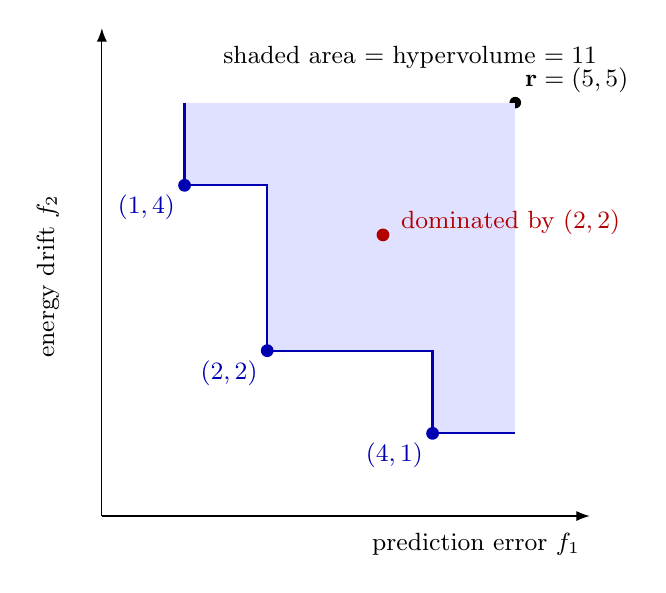
\begin{tikzpicture}[scale=1.05, font=\small]
\draw[-{Latex}] (0,0) -- (5.9,0) node[below left=1mm and 0mm] {prediction error $f_1$};
\draw[-{Latex}] (0,0) -- (0,5.9);
\node[rotate=90, anchor=south] at (-0.4,2.9) {energy drift $f_2$};
% reference point
\fill (5,5) circle (2pt) node[above right] {$\mathbf{r}=(5,5)$};
% dominated region (union of boxes), strips
\fill[blue!12] (1,4) rectangle (2,5);
\fill[blue!12] (2,2) rectangle (4,5);
\fill[blue!12] (4,1) rectangle (5,5);
% front points
\fill[blue!70!black] (1,4) circle (2.2pt) node[below left] {$(1,4)$};
\fill[blue!70!black] (2,2) circle (2.2pt) node[below left] {$(2,2)$};
\fill[blue!70!black] (4,1) circle (2.2pt) node[below left] {$(4,1)$};
% a dominated point
\fill[red!70!black] (3.4,3.4) circle (2.2pt);
\node[red!70!black, anchor=west] at (3.5,3.55) {dominated by $(2,2)$};
% front staircase
\draw[thick, blue!70!black] (1,5) -- (1,4) -- (2,4) -- (2,2) -- (4,2) -- (4,1) -- (5,1);
\node[anchor=west, align=left] at (1.35,5.55)
  {shaded area $=$ hypervolume $= 11$};
\end{tikzpicture}
\caption{The Hamiltonian study's objective plane (schematic, minimizing
both axes). The three blue trials are mutually incomparable and form the
current front; the red trial is dominated and argues for nothing. The
shaded region is everything the front dominates up to the reference
point, and its area, computed strip by strip in the text, is the
hypervolume~\eqref{eq:hv}: the one number that grows only when the front
genuinely advances or spreads.}
\label{fig:pareto}
\end{figure}

Hypervolume's cost is the catch. Computing and decomposing the dominated
region has time complexity that grows super-polynomially in the number of
objectives $m$ \citep{daulton2021qnehvi}, which in practice confines
hypervolume-driven methods to two to four objectives; beyond that,
scalarization-based methods take over. All of our current use cases sit
comfortably at $m \in \{2, 3\}$.

\section{Scalarize many times, or evolve a population}

The oldest trick converts the problem into many single-objective ones:
draw a weight vector, optimize the scalarized objective, repeat with
fresh weights, and collect the results. Whether this can even recover the
whole front depends on the scalarization, and the failure of the obvious
choice is geometric enough to draw.

Minimizing a weighted sum
$\sum_i w_i f_i$ with fixed positive weights means sliding the line (in
general, hyperplane) $\sum_i w_i f_i = c$ toward the origin until it last
touches the attainable region: the touching point is the minimizer. A
supporting line can only touch the region's convex hull, so for
\emph{any} positive weights, the minimizer of a weighted sum sits on the
convex hull of the attainable objective vectors, and Pareto points inside
a concave stretch of the front are never selected, whatever the weights
(Figure~\ref{fig:chebyshev}, left).

In the Hamiltonian study this is not
a curiosity: if the best balanced models happen to sit in a dent of the
front, every weighted-sum study we run will report only the two extremes,
a model that predicts well and leaks, and a model that conserves and
mispredicts, with the interesting compromises silently unreachable.

The scalarization of choice is therefore the Chebyshev form: with an
ideal point $\mathbf{z}^{\star}$ (each objective's best value, in
practice the best seen) and weights $w_i > 0$,
\begin{equation}
g_{\mathbf{w}}(\config)
= \max_{i = 1, \dots, m}\; w_i \left( f_i(\config) - z_i^{\star} \right),
\label{eq:chebyshev}
\end{equation}
the weighted \emph{worst} gap to the ideal rather than the weighted sum
of gaps. Its level sets are axis-aligned corners rather than lines, and a
corner can nestle into a concave dent that no line can touch
(Figure~\ref{fig:chebyshev}, right). The standard completeness statement
(sweeping positive weights with an appropriate true ideal point recovers
every Pareto point under convexity or boundary assumptions) is proven
using the true utopian vector, not a best-seen point; the latter is
usable in practice and provides a coverage advantage over weighted sums,
but it is an operational approximation rather than a theoretical
guarantee \citep{karl2023moo}.

ParEGO runs exactly this inside BO: each iteration
draws a random Chebyshev weight, scalarizes the observed data, and takes
an EI step on the result \citep{knowles2006parego};
random-scalarization bandits generalize the idea with guarantees
\citep{paria2019scalarization}. Scalarization scales gracefully in $m$
and composes with every single-objective engine we build, which is why
it remains the fallback when hypervolume machinery gets expensive.

\begin{figure}[t]
\centering
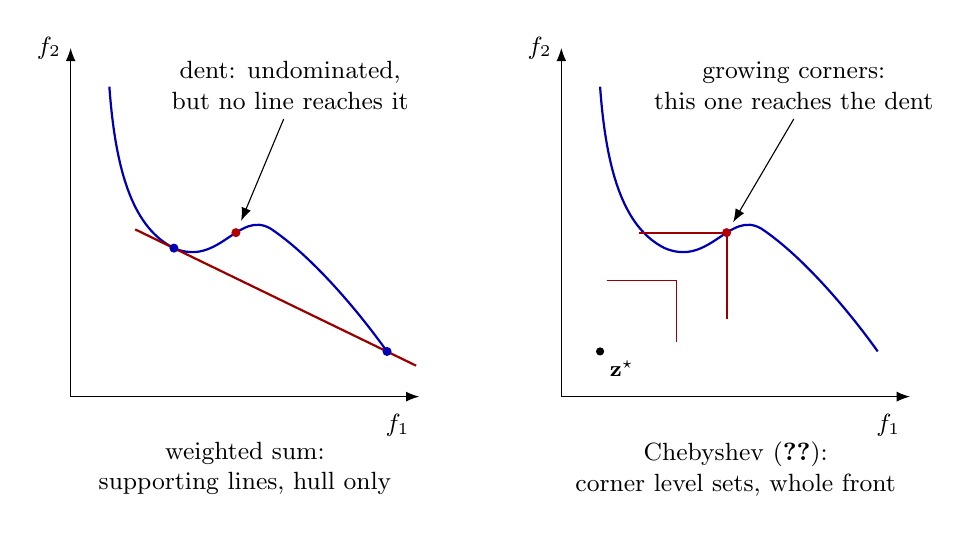
\begin{tikzpicture}[scale=0.82, font=\small]
% ---- left panel: weighted sum ----
\begin{scope}
\draw[-{Latex}] (0,0) -- (5.4,0) node[below left=1mm and 0mm] {$f_1$};
\draw[-{Latex}] (0,0) -- (0,5.4) node[left] {$f_2$};
% attainable region boundary: front with concave dent
\draw[thick, blue!70!black]
  (0.6,4.8) .. controls (0.7,3.4) and (1.0,2.6) .. (1.6,2.3)
  .. controls (2.3,2.0) and (2.6,2.9) .. (3.1,2.6)
  .. controls (3.7,2.2) and (4.4,1.4) .. (4.9,0.7);
% supporting line: hull chord through the two tangency points, spanning the dent
\draw[red!60!black, thick] (1.0,2.59) -- (5.35,0.48);
\fill[blue!70!black] (1.6,2.3) circle (2pt);
\fill[blue!70!black] (4.9,0.7) circle (2pt);
\fill[red!70!black] (2.56,2.54) circle (2pt);
\draw[-{Latex}] (3.3,4.3) -- (2.64,2.72);
\node[anchor=south, align=center] at (3.4,4.3) {dent: undominated,\\but no line reaches it};
\node[anchor=north, align=center] at (2.7,-0.55) {weighted sum:\\supporting lines, hull only};
\end{scope}
% ---- right panel: chebyshev ----
\begin{scope}[xshift=7.6cm]
\draw[-{Latex}] (0,0) -- (5.4,0) node[below left=1mm and 0mm] {$f_1$};
\draw[-{Latex}] (0,0) -- (0,5.4) node[left] {$f_2$};
\draw[thick, blue!70!black]
  (0.6,4.8) .. controls (0.7,3.4) and (1.0,2.6) .. (1.6,2.3)
  .. controls (2.3,2.0) and (2.6,2.9) .. (3.1,2.6)
  .. controls (3.7,2.2) and (4.4,1.4) .. (4.9,0.7);
% ideal point
\fill (0.6,0.7) circle (1.8pt) node[below right, font=\footnotesize] {$\mathbf{z}^{\star}$};
% corner level sets: vertex slides along the ray from the ideal point
\draw[red!60!black] (0.7,1.8) -- (1.78,1.8) -- (1.78,0.85);
\draw[red!60!black, thick] (1.2,2.54) -- (2.56,2.54) -- (2.56,1.2);
\fill[red!70!black] (2.56,2.54) circle (2pt);
\draw[-{Latex}] (3.6,4.3) -- (2.66,2.7);
\node[anchor=south, align=center] at (3.6,4.3) {growing corners:\\this one reaches the dent};
\node[anchor=north, align=center] at (2.7,-0.55) {Chebyshev~\eqref{eq:chebyshev}:\\corner level sets, whole front};
\end{scope}
\end{tikzpicture}
\caption{Why the obvious scalarization loses solutions (schematic). Left:
minimizing a weighted sum slides a line toward the origin; it can only
stop on the convex hull, so the concave stretch of the front is
unreachable for every choice of weights. Right: the Chebyshev
scalarization's level sets are corners, which can touch any Pareto point,
concave stretches included; sweeping its weights traces the whole front.}
\label{fig:chebyshev}
\end{figure}

Evolutionary methods attack the front directly with a population, using
dominance itself as the fitness signal. NSGA-II (the name abbreviates
non-dominated sorting genetic algorithm), the workhorse, sorts the
population into non-domination ranks (rank 1: the undominated; rank 2:
undominated once rank 1 is removed; and so on) and breaks ties within a
rank by crowding distance, a dispersion measure that prefers points in
sparsely covered stretches of the front, so selection pressure pushes
toward the front while spreading along it \citep{deb2002nsga2}. It needs
generous evaluation budgets, which multi-fidelity variants mitigate, and
it is the default multi-objective sampler in Optuna, so we get a tested
implementation for free when trials are cheap.

\section{Bayesian optimization of the front, one repair at a time}
\label{sec:mobo}

When a trial costs hours, the population's appetite disqualifies it,
and we are back in Chapter~\ref{sec:bayesian}'s situation: few,
expensive, noisy evaluations, and a surrogate that has to make each
one count. The machinery that results is best understood the way EI
was: one natural idea, then a short chain of repairs, each forced by
a failure that is easy to see once it is named.

\subsection{EHVI: expected improvement, paid in area}

The natural idea first. With one objective, EI asked how much a
candidate would improve on the incumbent, averaged over the
surrogate's uncertainty. With several objectives there is no single
incumbent; there is the staircase of Figure~\ref{fig:pareto}, and
progress means adding area to what it dominates. \emph{Expected
hypervolume improvement} (EHVI) therefore scores a candidate by the
expected increase of~\eqref{eq:hv} if we were to evaluate it: the
expected area of fresh territory.

One number makes the definition mechanical. Take the front of
Figure~\ref{fig:pareto} and a candidate configuration whose GP
posterior, say, puts half its mass at the outcome $(3, 1.5)$ and half
at $(3, 2.5)$. The first outcome lands in the dent and carves out the
$1 \times 0.5$ rectangle we computed earlier, an area of $0.5$; the
second is dominated by $(2,2)$ and adds nothing. The candidate's EHVI
is $0.5 \cdot 0.5 + 0.5 \cdot 0 = 0.25$. Every candidate gets such a
score, and the searcher proposes the maximizer, exactly EI's decision
logic with improvement measured in area. In practice the posterior is
a continuous Gaussian rather than two points, so the average is
estimated from posterior samples; nothing about the logic changes.

\subsection{Making it computable in batches: qEHVI}

Turning that definition into a working acquisition hits a geometric
wall. Each posterior sample asks for the area a proposed outcome adds
to a union of overlapping boxes, and we rarely propose one point at a
time: Chapter~\ref{sec:bayesian}'s batch argument applies unchanged,
since idle workers do not care that the objectives are plural. The
joint fresh area of $q$ proposals is the area of a union over a
union, and evaluating it naively by inclusion-exclusion sums over
subsets of the batch, a count that grows exponentially in $q$.

\citet{daulton2020qehvi} made the computation practical at batch
sizes above one. The dominated region is decomposed once per front
into disjoint boxes; each posterior sample's contribution is then a
sum over those pieces, exact rather than approximated, and the whole
estimator is differentiable in the candidate coordinates, so the
batch is optimized by gradient ascent like any other acquisition of
Chapter~\ref{sec:bayesian}.

\subsection{Noise bends the front: qNEHVI}

Now the failure our workloads force. Suppose one Hamiltonian trial,
of genuinely middling quality, draws a lucky seed and reports
$(1.8, 1.8)$. That phantom point dominates the honest compromise at
$(2,2)$, so the observed staircase bends around an outcome the true
objectives never produced. Every genuinely improving candidate is now
scored against territory the phantom already claims, EHVI near zero
across the board, and the study stalls defending a front that does
not exist. This is the winner's curse of
Section~\ref{sec:acquisition} again, with the lucky seed promoted
from incumbent to front member.

qNEHVI applies the same repair noisy EI used there: stop letting raw
observations define the front. The improvement is integrated over the
surrogate posterior at the observed points, so the front itself is
treated as uncertain, and a phantom member holds exactly as much
territory as the posterior believes it deserves
\citep{daulton2021qnehvi}. The same paper removed the remaining cost
wall, making joint batch proposals tractable where the naive
computation grew exponentially in batch size.

\subsection{Vanishing improvements again: qLogNEHVI}

The last repair is inherited. Late in a good study, almost no
candidate adds much area, and expected improvements shrink to the
magnitudes where Section~\ref{sec:acquisition} showed plain EI
underflowing to an exact floating-point zero; the underflow argument
applies verbatim to hypervolume improvements. The fix is the same
log-space computation, and the numerically stabilized variant
qLogNEHVI is the recommended default in the BoTorch ecosystem
\citep{ament2023logei}. The lineage that looked like alphabet soup at
the chapter's door is thus three cumulative repairs to one idea, and
the name now reads as a recipe: the q is the batch, the N is the noise
treatment, the Log is the underflow repair, and EHVI is the idea they
all serve.

\subsection{Two extensions on file}

Two further members solve problems we do not have yet, and one
paragraph each is enough to know when to reach for them. For
high-dimensional spaces, MORBO transplants the trust-region idea of
Figure~\ref{fig:turbo}: several local regions each pursue
hypervolume improvement with local models, coordinating through the
shared front \citep{daulton2022morbo}.

And when the objectives differ in evaluation cost, a profiler's
latency reading next to a full training run's accuracy, the
hypervolume knowledge gradient extends the machinery to decoupled
evaluations: it decides not only where to evaluate next but which
objective to measure there \citep{daulton2023hvkg}.

Our product needs qLogNEHVI as the premium
two-to-four-objective searcher and Chebyshev scalarization as the
cheap many-objective fallback; both ride on the same GP
infrastructure as Chapter~\ref{sec:bayesian}.

\section{Multi-objective meets multi-fidelity}

The savings of Chapter~\ref{sec:multifidelity} apply here too, with one
twist: promotion decisions need a ranking, and ``better'' is now the
partial order we started the chapter with. Promote-the-top-third is not
defined when the top third is not defined.

MO-ASHA resolves this with the layering NSGA-II already taught us.
Rung members are sorted into non-domination ranks, and rank 1 promotes
before rank 2. Ties within a front are broken by a dispersion rule in
objective space, either NSGA-II's crowding distance or an epsilon-net
that repeatedly picks the candidate farthest from those already
chosen; the top fraction then promotes as usual. In its authors'
experiments, promotion rules aware of the whole front beat scalarized
promotion in wall-clock terms \citep{schmucker2021moasha}, which is
the geometry of Figure~\ref{fig:chebyshev} surfacing inside the
scheduler: a scalarized promotion inherits the scalarization's
blind spots, rung by rung.

The repair travels. MO-DEHB applies the same
non-dominated-sorting-plus-crowding selection to DEHB's evolutionary
rungs \citep{awad2023modehb}, and the population family of
Chapter~\ref{sec:population} has its member too: MO-PBT swaps PBT's
scalar exploit ranking for non-dominated selection, evaluated on
trade-offs such as precision against recall and accuracy against
fairness \citep{dushatskiy2023mopbt}.

These are exactly the schedulers we will pair with cheap objectives
such as short-horizon energy drift in Hamiltonian networks. The drift
at rung 1 is cheap to measure and, per Figure~\ref{fig:curves}'s
warning, worth a pilot check that its early rankings mean anything
before we let it cull.

\section{Constraints and preferences}

Two pragmatic variants round out the toolkit. Hard constraints (memory
ceilings, latency budgets, a minimum acceptable return) are handled by
weighting acquisitions with the modeled probability of feasibility. A
candidate whose acquisition score is $0.8$ but whose modeled chance of
fitting under the memory ceiling is $0.3$ counts as
$0.8 \times 0.3 = 0.24$: still on the table, discounted by exactly its
chance of being usable. Noisy-observation treatments of the same idea
exist \citep{letham2019noisyei}, and trust-region versions scale it to
many constraints at once \citep{eriksson2021scbo}.

Preferences short of hard
constraints (``we care about drawdown roughly twice as much as
turnover'') can be encoded by restricting the reference point or the
weight distribution of the scalarization; this is cheap, transparent,
and usually all a practitioner wants. We recommend exposing both, and
resisting anything more elaborate until a real use case demands it.

\section{The evidence, and the check it still lacks}
\label{sec:mo-evidence}

Weighed the way Section~\ref{sec:bo-evidence} taught us to weigh, this
chapter's support has an unusual profile. A larger share than usual is
mathematics that can be checked at a desk; the experiments that exist
are the method authors' own; and the tier that anchored the last two
chapters, an independent budget-matched comparison by outsiders, has no
counterpart here that our literature sweeps could find. Each of those
three facts shapes a different part of the decision box.

Start with what the mathematics settles on its own. The weighted-sum
blind spot is a one-page supporting-hyperplane argument, reproduced in
full above; the Chebyshev form's ability to reach every Pareto point is
its geometric mirror \citep{karl2023moo}; hypervolume strictly
increases exactly when the front advances or spreads, the worked
computation under Figure~\ref{fig:pareto}; and the cost of decomposing
the dominated region grows super-polynomially in the number of
objectives \citep{daulton2021qnehvi}, which draws the two-to-four
boundary. These four facts alone decide the exclusion of weighted
sums, the inclusion of Chebyshev as the fallback, the choice of
progress score, and the boundary past which the premium searcher
gives way. No experiment is being asked to carry those verdicts,
which is fortunate, because experiments of the decisive kind are the
scarce resource here.

The experiment behind the premium pick is the qNEHVI paper's own
evaluation, and its design earns a close look because of one choice:
noise is a first-class experimental axis rather than a footnote. The
comparison spans the modern acquisition families (information-based
PESMO, MESMO, and PFES, the diversity-guided DGEMO, scalarizing
TSEMO and MOEA/D-EGO, Thompson-sampling and plug-in variants of the
hypervolume line) on synthetic and real-world problems, with
observation noise scaled as a percentage of each objective's range
and pushed to twenty percent, a regime the authors note prior noisy
work had probed only at one percent \citep{daulton2021qnehvi}.

Every
method degrades as noise rises; qNEHVI degrades least and leads the
noisy benchmarks in both sequential and batch settings, at
competitive wall time thanks to the cached box decompositions. This
is the authors' own arena, so the selection-bias caution applies, but
two things temper it. The winning move is the same
integrate-over-the-posterior treatment whose single-objective version
carried the noise evidence of Chapter~\ref{sec:bayesian}, arriving
here as transferred machinery rather than a fresh conjecture. And the
axis the authors chose to stress, heavy observation noise, is not a
flattering backdrop chosen for the method; it is the axis our
workloads actually live on, seed-noisy RL returns and
effective-sample-size measurements.

The experiment behind the multi-objective early-stopper is the
MO-ASHA paper's, three tasks chosen to be genuinely unlike one
another: architecture search on a tabular benchmark whose exact
Pareto front is knowable, fairness-accuracy trade-offs on a standard
dataset, and Transformer language-model tuning, all run as
thirty-minute wall-clock races with objectives normalized by
empirical quantiles so that no objective's units dominate by
accident \citep{schmucker2021moasha}. The comparison that matters
inside it: promotion rules that see the whole front (non-dominated
sorting with a dispersion tie-break) against three scalarized
promotion rules, each given a hundred random weight vectors. The
front-aware rules win in wall-clock hypervolume, which is the
experimental echo of the geometry above: a scalarized promotion
inherits the scalarization's blindness, rung by rung.

What this family lacks is the third tier: no independent,
budget-matched, seed-split study of multi-objective tuners on live
training runs surfaced in our audit, nothing that does for this
chapter what \citet{eimer2023hyperparameters} does for
Chapters~\ref{sec:multifidelity} and \ref{sec:population}. The
authors' arenas are also not ours; fairness datasets and tabular
architecture-search benchmarks are a long way from Hamiltonian
rollouts and sampler diagnostics.
The consequence is not paralysis, because the geometry and the
transferred noise machinery carry most of the weight; the
consequence is that our own validation suite has to play the role
the literature has not filled yet, and the falsification criterion
below is written accordingly.

\section{The verdicts, argued from four angles}
\label{sec:mo-angles}

The chapter recommends qLogNEHVI as the premium searcher inside the
two-to-four-objective boundary, Chebyshev scalarization as the cheap
universal fallback, NSGA-II by wrapping for bulk cheap trials, and
MO-ASHA as the early-stopper. Four angles, one verdict.

From geometry: the load-bearing exclusions and boundaries follow
from arguments a reader can verify without trusting a single
benchmark: the hull argument disqualifies weighted sums, the corner
level sets qualify Chebyshev, and the decomposition cost draws the
objective-count boundary. Decisions anchored this way are immune to
the selection-bias worries that haunt benchmark-anchored ones, and
the experiments are needed only for the choices the geometry leaves
open.

From economics: committing to weights before searching is assuming
the exchange rate the study exists to discover; returning a front is
handing the decision-maker the actual menu and letting preference be
exercised when the trade-off is visible and the stakes are known.
The Chebyshev-versus-weighted-sum contrast is the familiar one
between corner-shaped and linear indifference curves, and the dent
in Figure~\ref{fig:chebyshev} is precisely where a linear
indifference curve misreports what is attainable. A reader who
would not let a colleague assume a client's utility function before
seeing the budget set should not let a tuner do it either.

From evidence: the experiments that exist, though author-run, stress
the failure modes that matter to us rather than flattering ones,
heavy observation noise for the acquisition and wall-clock
promotion honesty for the scheduler, and their findings are the
experimental shadows of theorems taught above rather than
free-standing claims. Nothing in this family's record contradicts
any result we verified in the single-objective chapters, and the
missing independent tier is named rather than papered over.

From operations: the whole chapter rides rails already bought. The
premium searcher runs on Chapter~\ref{sec:bayesian}'s GP stack and
inherits its LogEI repair; the evolutionary default arrives by
wrapping Optuna, whose maintenance we audited
(Chapter~\ref{sec:libraries}); the early-stopper is a week of work
on top of our ASHA; and the objective-count boundary is enforceable
in software. The marginal cost of honest multi-objective tuning,
given the rest of the product, is weeks, which changes the
include-or-defer calculus in its favor.

And the falsification criterion, stated in advance: the validation
suite adopts the Hamiltonian study, prediction error against energy
drift, as a pinned two-objective task, run at matched budgets across
seeds with final hypervolume and its uncertainty reported. The
premium searcher must beat random-weight Chebyshev and the wrapped
NSGA-II there; MO-ASHA's cheap early signal, short-horizon drift,
must pass the rank-correlation pilot of
Chapter~\ref{sec:multifidelity} before it is allowed to cull; and if
the cheap fallback matches the premium searcher on our tasks, the
premium tier is demoted to an option, the same rule the
single-objective chapters applied to themselves.

\begin{decisions}
\noindent\textbf{Decisions from this chapter.} Pick by the number of
objectives, the noise level, and the price of a trial.
\begin{itemize}[leftmargin=1.3em, itemsep=2pt]
\item \textbf{qLogNEHVI on BoTorch} (include; the premium searcher;
weeks). For two to four objectives with expensive, noisy trials, which
is precisely the Hamiltonian and finance profile. It is the noise-aware,
numerically repaired member of the hypervolume family, and the BoTorch
ecosystem's own recommended default \citep{daulton2021qnehvi,
ament2023logei}. Beyond four objectives its hypervolume arithmetic
becomes the bottleneck, so the default switches to scalarization there;
treat that as a calibrated cutoff on published complexity results
rather than a prohibition, and make it a configurable threshold whose
override is recorded in the study's audit trail.
\item \textbf{Chebyshev scalarization with random weights} (include;
days). The cheap fallback that composes with every single-objective
engine we own and has better coverage than weighted sums: it can reach
concave stretches of the front that weighted sums cannot
(Figure~\ref{fig:chebyshev}). Completeness under random weights
requires the true ideal point and additional assumptions; the
operational approximation using best-seen values gives better coverage
in practice without the theoretical guarantee. This is also the answer
for five or more objectives.
\item \textbf{Plain weighted sums as a product default} (exclude).
They silently discard the concave stretch of the front; if a user
truly has fixed exchange rates, they have a single-objective problem
and should declare it as one.
\item \textbf{NSGA-II by wrapping Optuna} (include; free). For cheap
trials in bulk, the evolutionary route is a tested default we get by
wrapping, not building.
\item \textbf{MO-ASHA with veto gates} (build; about a week over
ASHA). The multi-objective early-stopper, and the veto machinery
doubles as the correctness gate the sampler workload needs
(Chapter~\ref{sec:workloads}).
\item \textbf{MORBO and the hypervolume knowledge gradient} (defer).
Each answers a situation we do not yet have: very high-dimensional
Pareto search, and objectives measurable separately at different
prices. Revisit on demand.
\end{itemize}
\end{decisions}

\section{What would overturn these verdicts}

qLogNEHVI's tier-1 inclusion depends on V09: if it cannot beat
random-weight Chebyshev scalarization and the wrapped NSGA-II on the
Hamiltonian task by a margin that justifies its complexity, it is
demoted to an option. MO-ASHA's veto gates are tied to V10 and V13:
if cheap fidelity signals (short-horizon drift) fail the
rank-correlation pilot, or if a veto-failing configuration ever gets
promoted in validation, the mechanism is disabled and full-fidelity
MO defaults to the scalarized floor. Weighted-sum exclusion is
reopened if the convexity assumption turns out to hold on our tasks,
which V09's results will show. MORBO's deferral is reconsidered when
trust-region BO is proven and the Pareto-aware TR extension becomes
a marginal cost rather than a second research bet.

\chapter{Using what we already know: priors, transfer, and the price of a trial}
\label{sec:transfer}

A tuner that starts every study from ignorance wastes its first dozen trials
rediscovering folklore: learning rates live near $3 \times 10^{-4}$, discount
factors near $0.99$, dropout rarely helps reinforcement learning. Every GP in
Chapter~\ref{sec:bayesian} began with a zero-mean prior that believes
nothing; every project lead we serve believes a great deal, and is usually
right. We tune the same families of models over and over, so encoded
experience is the cheapest compute we own. The literature offers three
grades of it, in increasing order of machinery, plus a fourth option that
replaces search entirely at large scale.

\section{Expert priors over the optimum}

The lightest grade lets a human say where the optimum probably lies. In
$\pi$BO, the user supplies a prior density $\pi(\config)$ over the
\emph{location of the best configuration} (not over function values, which
is the GP's job), and the acquisition function is multiplied by that
density raised to a power that decays with the number of observations,
\begin{equation}
\alpha_n^{\pi}(\config)
\;=\; \alpha_n(\config) \cdot \pi(\config)^{\beta / n},
\label{eq:pibo}
\end{equation}
where $\alpha_n$ is any standard acquisition (EI in the paper), $n$ counts
observations, and $\beta$ sets how long the advice matters
\citep{hvarfner2022pibo}.

The design reads directly off the formula. Early
on ($n$ small) the exponent is large, the prior term dominates, and the
search concentrates where the expert pointed; as evidence accumulates the
exponent shrinks toward zero, $\pi(\config)^{\beta/n} \to 1$ for every
$\config$ in the prior's support, and the acquisition converges back to
its data-driven self on that support (Figure~\ref{fig:pibo}). Points
assigned zero prior probability stay at zero. The decay is what makes
the mechanism safe: the authors prove it preserves standard convergence
behavior, and show large early gains when the prior is good and mild
losses when it is wrong, since a wrong prior is overruled at the rate
evidence arrives. A confidently wrong expert costs the study its opening
moves, not its conclusion.

\begin{figure}[t]
\centering
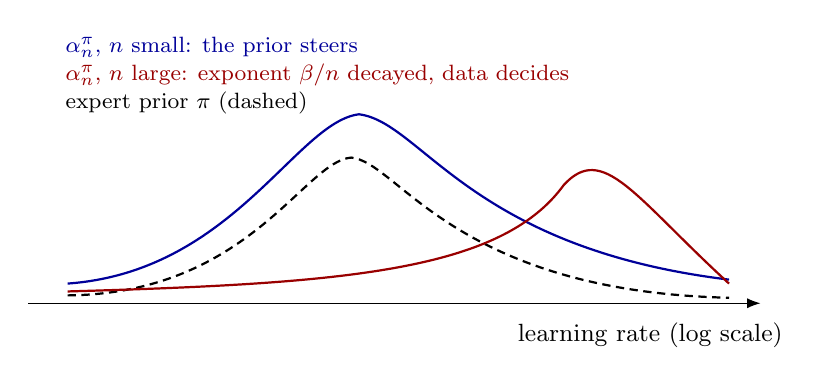
\begin{tikzpicture}[scale=1.0, font=\small]
\draw[-{Latex}] (0,0) -- (9.3,0);
\node[anchor=north] at (7.9,-0.12) {learning rate (log scale)};
% prior density
\draw[thick, densely dashed]
  (0.5,0.1) .. controls (2.8,0.12) and (3.5,1.8) .. (4.1,1.85)
  .. controls (4.7,1.8) and (5.4,0.15) .. (8.9,0.07);
% early acquisition: pulled toward prior
\draw[thick, blue!60!black]
  (0.5,0.25) .. controls (2.6,0.4) and (3.4,2.3) .. (4.2,2.4)
  .. controls (5.0,2.3) and (5.6,0.7) .. (8.9,0.3);
% late acquisition: data-driven peak elsewhere
\draw[thick, red!60!black]
  (0.5,0.15) .. controls (4.0,0.25) and (6.0,0.4) .. (6.8,1.5)
  .. controls (7.3,2.05) and (7.7,1.35) .. (8.9,0.25);
% legend, top left, clear of all three curves
\node[blue!60!black, anchor=west, font=\footnotesize] at (0.35,3.25)
  {$\alpha^{\pi}_{n}$, $n$ small: the prior steers};
\node[red!60!black, anchor=west, font=\footnotesize] at (0.35,2.9)
  {$\alpha^{\pi}_{n}$, $n$ large: exponent $\beta/n$ decayed, data decides};
\node[anchor=west, font=\footnotesize] at (0.35,2.55)
  {expert prior $\pi$ (dashed)};
\end{tikzpicture}
\caption{The $\pi$BO mechanism~\eqref{eq:pibo} over a study's lifetime
(schematic). The expert's prior (dashed) multiplies the acquisition with
an exponent that decays as observations arrive: early proposals
concentrate where the expert pointed, late proposals go where the data
says, and a wrong prior is forgotten rather than obeyed.}
\label{fig:pibo}
\end{figure}

PriorBand carries the same idea into the multi-fidelity world of
Chapter~\ref{sec:multifidelity}, where the object being steered is not
one acquisition but a stream of configurations entering ASHA-style rungs.
Each new configuration is drawn from a portfolio mixing three samplers:
uniform exploration, the user prior, and local perturbations of the
current incumbent, with the mixing weights depending on the rung. The
prior is trusted more at higher rungs, where evaluations are expensive
and the expert's opinion matters most, and the incumbent component is
switched on only once enough evidence has accumulated, which is what
protects the method against a confidently wrong prior
\citep{mallik2023priorband}. Priors of this kind should be a first-class
field in our search-space schema from day one: every project lead we
serve has them, and both mechanisms are simple to implement over
components we are building anyway. The prior is also the natural home
for the folklore this chapter opened with; writing
$\pi(\config)$ down once beats re-teaching it to every study.

\section{Transfer from our own past studies}

The second grade learns from previous tuning studies instead of asking a
human. The robust end of this spectrum is unglamorous and effective:
initialize a new study with configurations that ranked well on similar
past tasks \citep{feurer2015metalearning}, or combine surrogates fit to
past tasks into an ensemble whose weights reflect how well each past
task's surrogate predicts the current one, comparing on ranks so that
tasks with different loss scales can vote together
\citep{feurer2018rgpe}. Because our product will keep every trial of
every study in one store (Chapter~\ref{sec:architecture}), the warm
start costs a database query: the run store is Figure~\ref{fig:loop}'s
bottom box earning its place.

The research frontier goes further and meta-learns the surrogate itself,
and the vehicle deserves a proper introduction because it has appeared
twice already (ifBO in Chapter~\ref{sec:multifidelity}) and will appear
again. A \emph{prior-fitted network} (PFN) is a transformer trained once,
offline, on millions of synthetic datasets drawn from a chosen prior over
functions. At use time it is shown the current study's observed
(configuration, score) pairs as context, and it outputs a predictive
distribution for new configurations in a single forward pass.

Why that works is the part worth pausing on. Training on draws from
the prior teaches the network to approximate the posterior predictive
distribution under that prior, so the expensive part of Bayesian
inference is paid once, by the pre-trainer, rather than at every step
of every study. Where the GP of Section~\ref{sec:gp} refits
\eqref{eq:mll} inside the loop, a PFN just reads its context. The
model class changed; the economics changed with it.

PFNs4BO demonstrates the swap directly, pre-training PFNs that mimic
GP and Bayesian-neural-network surrogates and slotting them into
standard BO \citep{muller2023pfns4bo}.

OptFormer showed the scale endgame: a transformer trained on hundreds
of thousands of tuning trajectories from Google's Vizier service
imitates several tuners and improves on them when combined with
expected improvement \citep{chen2022optformer}.

The same idea specialized to learning curves gives ifBO's freeze-thaw
surrogate (Chapter~\ref{sec:multifidelity}), and the line is still
moving, with in-context amortization now reaching the acquisition
function itself \citep{rakotoarison2026alphapfn}.

These pre-trained surrogates are the most credible path to tuners
that get smarter as our run store grows, and one of them (ifBO) ships
with usable code today. We rate them a second-wave investment:
valuable, but only after the plain warm start is in place and
earning.

\section{Cost-aware search}

The third grade treats the price of a trial as part of the decision.
Trials rarely cost the same: in the running example, doubling network
width or unroll length can quadruple wall-clock, so two candidates with
equal expected improvement can differ fourfold in what they cost to
evaluate, and an acquisition that ignores this will happily spend its
budget in the expensive corner of the space. The classical repair prices
the acquisition in the right currency: improvement per unit cost,
$\alpha_{\mathrm{EI}}(\config) / c(\config)$, with $c$ a model of trial
cost, already present in \citet{snoek2012practical} as expected
improvement per second. CArBO refines it with an explicit cheap-first
initialization and a cost-cooling schedule, dividing by
$c(\config)^{\alpha}$ with an exponent that anneals from one toward
zero over the budget, so that early exploration favors cheap points and
the endgame, where only the best candidates remain, ignores cost
\citep{lee2020carbo}; the annealing acknowledges that a bargain matters
when we are learning the space and stops mattering when we are
choosing the winner.

CARBS pushes cost-awareness to its logical end for scaling studies. It
maintains a Pareto front in the plane of cost versus performance, the
machinery of Chapter~\ref{sec:moo} with cost promoted to a full
objective, and searches locally around that front: separate Gaussian
processes model performance, cost, and the front's shape, candidates are
Gaussian perturbations of current Pareto members, and the acquisition is
expected improvement relative to the front weighted by expected cost, so
the method tunes hyperparameters \emph{while} the model grows and emits
a scaling law for every hyperparameter as a byproduct. Its authors
demonstrate it by reproducing the Chinchilla scaling result for language
models and by solving the full ProcGen benchmark with a tuned but
otherwise plain PPO \citep{fetterman2023carbs}. For our fixed-size
studies, EI-per-cost with cost cooling is the sensible default; a
CARBS-style cost frontier becomes interesting the day we tune models
meant to be scaled up afterward.

\section{When not to search at all: transfer across scale}

For large networks there is a fourth option that is not search. The
maximal update parametrization ($\mu$P) rescales initialization and
per-layer learning rates so that the size of each layer's update stays
controlled as network width grows; under that parametrization the optimal
values of many hyperparameters become approximately invariant to width,
so one tunes a small proxy model and transfers the result to the wide
target ($\mu$Transfer). Its authors validated the recipe by
outperforming the published BERT-large and GPT-3 6.7B settings while
spending a few percent of one pretraining run on tuning
\citep{yang2022mutransfer}. The claim's boundary is part of the result:
the theory covers width; transfer across depth, batch size, and training
horizon is empirical, with stated failure cases (regularization
hyperparameters do not transfer, and depth transfer breaks for
post-layer-norm transformers), and follow-up parametrizations have since
extended the depth story \citep{dey2025completep}.

More recent LLM-era work makes the third regime of
Figure~\ref{fig:regimes} explicit, fitting power laws for optimal
hyperparameters as functions of scale and turning the largest tuning
problems into curve lookups: compute-dependent learning-rate and
batch-size laws appear in the DeepSeek LLM report \citep{deepseek2024llm},
learning-rate dependence on the token horizon has its own fitted law
\citep{bjorck2025tokenhorizon}, weight decay and batch size get the same
treatment \citep{bergsma2025powerlines}, and a dedicated preprint fits
joint optimum surfaces across model and data size \citep{li2025steplaw}.

We track this line in Chapter~\ref{sec:roadmap} as guidance to encode
rather than an algorithm to implement: the laws enter our product as
priors and sanity checks, not as a searcher.

\begin{figure}[t]
\centering
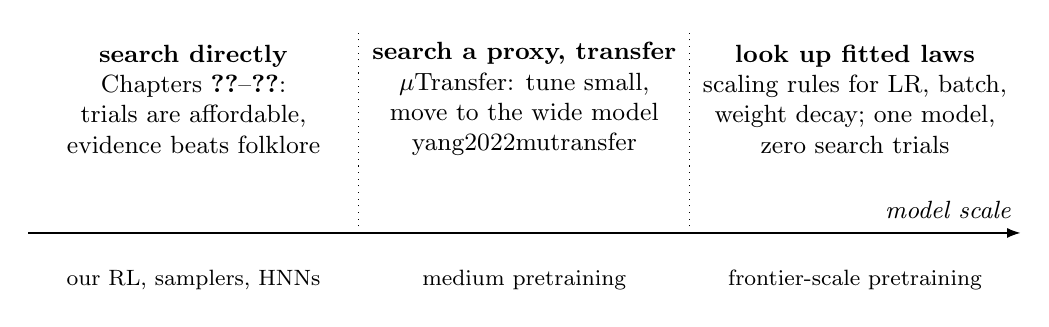
\begin{tikzpicture}[font=\small]
\draw[-{Latex}] (0,0) -- (12.6,0) node[above left=0.6mm and 0mm, font=\small\itshape] {model scale};
\foreach \x in {4.2,8.4} \draw[dotted] (\x,0) -- (\x,2.6);
\node[align=center] at (2.1,1.7) {\textbf{search directly}\\Chapters~\ref{sec:bayesian}--\ref{sec:moo}:\\trials are affordable,\\evidence beats folklore};
\node[align=center] at (6.3,1.7) {\textbf{search a proxy, transfer}\\$\mu$Transfer: tune small,\\move to the wide model\\\citep{yang2022mutransfer}};
\node[align=center] at (10.5,1.7) {\textbf{look up fitted laws}\\scaling rules for LR, batch,\\weight decay; one model,\\zero search trials};
\node[anchor=north, font=\footnotesize] at (2.1,-0.35) {our RL, samplers, HNNs};
\node[anchor=north, font=\footnotesize] at (6.3,-0.35) {medium pretraining};
\node[anchor=north, font=\footnotesize] at (10.5,-0.35) {frontier-scale pretraining};
\end{tikzpicture}
\caption{The three tuning regimes by model scale. Everything before this
chapter lives in the left band. As trials become unaffordable, search
moves onto small proxies whose optima provably or empirically transfer,
and at the largest scales it gives way to fitted scaling laws. A good
tuner should know which band a study is in and say so.}
\label{fig:regimes}
\end{figure}

The strategic point for the product is the figure's caption: at small
scale we search, at medium scale we search on proxies and transfer, and
at large scale search gives way to parametrization and extrapolation. A
good tuner should know which regime it is in and say so.

\section{The evidence, and how the failure mode was tested}
\label{sec:prior-evidence}

Every claim in this chapter has the same shape: knowledge from outside
the study, an expert's hunch, a past study, a smaller model, someone
else's fitted law, can safely be spent inside it. For claims of that
shape the success story is cheap to produce and nearly beside the
point, because of course good advice helps. The evidence that matters
is what happens when the imported knowledge is wrong, and the reason
this chapter's verdicts lean confident is that its sources, unusually,
tested exactly that.

The $\pi$BO experiments are built around controllable advice quality.
On a toy function and two surrogate tuning tasks, where the true
optimum is known and priors of any desired quality can be
manufactured, the authors ran the spectrum from accurate to
``purposefully detrimental,'' the wrong prior being a narrow density
parked in the worst region of the space \citep{hvarfner2022pibo}.

The findings match the mechanism read off
formula~\eqref{eq:pibo}: strong priors buy large early gains, and
under sabotage the method climbs back to roughly the regret of its
prior-free baseline, while the baseline that trusts the prior only at
initialization keeps paying for it. The trade-off is stated rather
than hidden: a larger $\beta$ extracts more from good advice and
forgives bad advice more slowly.

The upside case is demonstrated
separately on a deep-learning pipeline, a 12.5-fold time-to-accuracy
speedup over vanilla BO and a new best validation accuracy for that
pipeline. Author-run experiments, as usual in this document's
sources; what tempers the caution here is that the safety half of the
claim is also a theorem (the exponent $\beta/n$ dies as evidence
arrives, dragging the acquisition back to its data-driven self), so
the experiment confirms an argument the reader can check rather than
substituting for one.

PriorBand's evaluation had to build its own arena first, a benchmark
suite in which priors are part of the task definition rather than an
afterthought: synthetic multi-fidelity surfaces plus image and
language tasks derived from recorded large-model training runs, each
equipped with good and deliberately bad priors, run at the small
budgets that define deep-learning tuning
\citep{mallik2023priorband}. The motivating ablation is the honest
part: naively biasing Hyperband's sampler toward the prior wins when
the advice is good and burns exactly proportional budget when it is
bad, while a half-random hedge is robust but never competitive, and
the rung-dependent trust schedule is the repair that keeps both
properties. One design detail is worth copying into our own suite:
every prior-using method in the comparison had the prior's mode
evaluated first, so nobody wins merely by being handed the expert's
best guess. Across tasks and prior qualities, PriorBand ranked most
consistently at the top.

The transfer-across-scale evidence is differently shaped, and
stronger for it. $\mu$Transfer's headline test pitted the recipe
against external baselines its authors did not set: the published,
expert-tuned settings of BERT-large and GPT-3 6.7B, beaten while
spending a few percent of one pretraining run on proxy-model tuning
\citep{yang2022mutransfer}, with the non-transfers (regularization
strengths, depth under post-layer-norm) reported in the same paper.
CARBS makes its case the same way, by reproducing a famous external
result, the Chinchilla compute-optimal scaling law, and by solving
the full ProcGen benchmark with an otherwise plain PPO
\citep{fetterman2023carbs}. Replication of results the authors do
not own is the closest thing this literature has to the
adversarial arena of Section~\ref{sec:bo-evidence}, and both
transfer claims clear it.

The last tier is the one we deliberately did not audit. The
scaling-law papers of the previous section report fitted power laws
whose estimation we have not checked, and nothing in our product is
allowed to depend on their exactness: they enter as priors and
sanity checks, which is weight their evidentiary status can carry
even if a particular fit is off. The demotion is a statement about
our audit, not an accusation about their work.

\section{The ordering, argued from four angles}
\label{sec:prior-angles}

The chapter's verdict is an ordering: priors and warm starts first,
cost-aware acquisition alongside, pre-trained surrogates adopted
rather than trained, scaling knowledge encoded rather than
implemented. Four angles converge on it.

From mechanism: the safety properties that make priors acceptable as
a default are structural, not empirical. The decay exponent in
\eqref{eq:pibo} guarantees the expert's influence is transient;
PriorBand's incumbent component stays off until evidence justifies
it; in both, the worst case of bad advice is a study's opening
moves. Features whose failure modes are bounded by construction can
be on by default; features whose failure modes are empirical
questions cannot. That one sentence sorts most of the decision box.

From evidence: the sources tested the sabotage case, not only the
success case, and the transfer methods validated against external
baselines their authors did not control. Where our own audit is
thinner, the scaling-law fits, the verdict steps down to
encode-as-guidance in lockstep. Nothing here asks the reader to
extend more trust than the checked evidence covers.

From economics: encoded experience is the cheapest compute we own.
A written-down prior converts folklore into an asset that every
study inherits for free; the run store turns past studies' sunk
compute into a warm start that costs a query; and EI-per-cost simply
prices candidates in the currency the cluster actually charges,
improvement per unit cost rather than improvement per trial. The
whole chapter is arbitrage on knowledge the organization has already
paid for once.

From operations: the entire first wave is days of work riding
components that earlier chapters build anyway, a multiplier on the
acquisition, a query over the run store, a divisor on the
acquisition, and the single costly commitment, making the prior a
first-class field of the search-space schema, costs nearly nothing
on day one and a migration if retrofitted later. Adopting ifBO's
published surrogate rather than training our own keeps a research
program off the product's critical path.

And the falsification criterion, stated in advance: the validation
suite reruns the pinned tasks under three conditions, no prior, the
folklore prior, and a deliberately wrong prior in $\pi$BO's sense,
at our routine budgets. The prior-weighted searcher must beat its
prior-free self under the folklore prior and must recover to the
prior-free final, within noise, under the wrong one; if bad advice
costs more than the opening moves on our workloads, prior weighting
is demoted from default to opt-in. The warm start faces its own
test the day the run store holds enough studies: measured trial
savings on a new study of a familiar family, or it stays a query we
offer rather than a step we perform.

\begin{decisions}
\noindent\textbf{Decisions from this chapter.} Ordered by payoff per
week of engineering, which is the honest ranking here.
\begin{itemize}[leftmargin=1.3em, itemsep=2pt]
\item \textbf{$\pi$BO's prior-weighted acquisition} (include; days).
Formula~\eqref{eq:pibo} is a few lines over the Tier 0 GP searcher,
every project lead has a prior to give it, and its built-in decay
means bad advice costs a study its opening moves rather than its
conclusion, \emph{provided the prior does not assign zero probability
to the true region}. The search-space schema should therefore require
a lower-bounded mixture or explicitly nonzero support everywhere, so
that wrong advice can be overruled by evidence \citep{hvarfner2022pibo}.
Highest value density in the document under that guard.
\item \textbf{PriorBand} (include; one to two weeks). The same idea
where our savings actually live, the multi-fidelity rungs; the
rung-dependent portfolio is what keeps a confidently wrong prior from
doing damage \citep{mallik2023priorband}.
\item \textbf{Warm starts from the run store} (include; days). A
ranked query over past studies \citep{feurer2015metalearning}. The
prerequisite is the run store itself, which Tier 0 builds regardless.
\item \textbf{RGPE-style surrogate ensembles} (second wave). Real
gains, but only once the store holds enough completed studies to
ensemble; building it before the data exists would be decoration.
\item \textbf{Pre-trained surrogates (PFN family)} (adopt one, build
none). We take ifBO's published pre-trained model as our
learning-curve surrogate (Chapter~\ref{sec:multifidelity}) and train
nothing ourselves; OptFormer-scale training runs are a research
program, not a package feature.
\item \textbf{EI-per-cost with cost cooling} (include; days). One
division and one annealing exponent on top of the GP searcher,
\emph{dividing by a predicted cost} rather than the realized cost the
executor measures \citep{lee2020carbo}. A second GP fits log
wall-clock time to configuration coordinates, refitting on the same
cadence as the performance surrogate, with failed and killed trials
entered as censored observations. The roadmap details the cold-start
and calibration-logging protocol.
\item \textbf{CARBS-style cost frontier} (hold). Becomes relevant the
day a project tunes a model that is destined to be scaled up; none is
on the books today \citep{fetterman2023carbs}.
\item \textbf{$\mu$P and the scaling-law literature} (encode, do not
implement). These enter the package as priors, defaults, and sanity
checks on the regime map of Figure~\ref{fig:regimes}, not as a
searcher; at our current scales they advise rather than replace
search.
\end{itemize}
\end{decisions}

\section{What would overturn these verdicts}

The $\pi$BO prior weight's default-on status depends on V11: if
gains under a good prior do not materialize, or if recovery from a
wrong prior takes longer than the no-prior baseline, the feature is
demoted to opt-in. PriorBand's inclusion holds as long as its ASHA
dependency does; if ASHA is demoted, PriorBand's rung-sampling
portfolio loses its substrate. Warm starts (V12) mature as the store
fills; if trial savings remain undetectable after the store holds
dozens of studies, the query surface is re-examined. EI-per-cost's
inclusion assumes executor cost metering is cheap; if metering
overhead becomes visible in profiling, the feature becomes opt-in.
RGPE's second-wave hold is lifted when an ensemble that cheap proves
itself on public suites, at which point the evidence section is
updated and a new decision box opened.


\part{From methods to our system}
\chapter{Our workloads, concretely}
\label{sec:workloads}

The preceding chapters organized the literature by method. This one flips
the table and asks, for each family of work in our repositories, what the
evidence says we should actually do. Each section ends in a concrete
default: the study we would configure today, with the chapters that
justify each choice.

\section{Reinforcement learning}

The controlled evidence base here is unusually good, and we have already
leaned on it: \citet{eimer2023hyperparameters} tuned PPO, SAC, and DQN
across eleven environments with matched budgets and seeds. Four of their
findings should directly shape our defaults. First, hyperparameter
importance is broad but concentrated: almost every swept knob mattered
somewhere, importance analysis attributed most variance to one or two knobs
per environment, and which knobs those were changed across environments, so
the search space should include everything plausible rather than a
hand-picked pair. This is the effective-dimensionality picture of
Figure~\ref{fig:gridrandom} with a twist: the important axes exist, but we
cannot know in advance which they are, which is precisely the situation
where random-style coverage of every axis, and GP lengthscales that learn
to switch axes off (Section~\ref{sec:gp}), earn their keep.

Second, the
response surfaces themselves looked smooth and well behaved; the
difficulty of tuning RL comes overwhelmingly from seed noise, not from a
pathological objective. That is good news for every surrogate in
Chapter~\ref{sec:bayesian}, and it aims the engineering effort at noise
handling (the noise-aware acquisitions of
Section~\ref{sec:acquisition}) rather than at exotic models.

Third, the
seed noise is severe enough to corrupt conclusions: configurations tuned
on one seed transferred poorly, incumbents evaluated on tuning seeds
overstated test performance several-fold in the worst cases, and their
protocol of tuning on a handful of seeds and reporting on disjoint test
seeds is the minimum honest practice.

Fourth, at budgets of ten to
sixty-four full training runs, DEHB was the most dependable tuner, with
random search respectable and population methods behind; the population
methods' natural habitat is the large-parallelism regime of
Chapter~\ref{sec:population}, where BG-PBT's own experiments live.

Assembled into a default: an RL study below a few dozen full-run
equivalents uses DEHB (or BO plus ASHA) over the full plausible space,
evaluates each candidate on several tuning seeds, reports on disjoint
test seeds, and holds the tuning budget fixed in any method comparison;
a study with eight or more dedicated full-length workers and a
schedule-shaped question upgrades to the population line, PB2-Mix now
and BG-PBT when we build it.

The broader AutoRL literature, surveyed by
\citet{parkerholder2022autorl}, adds the framing that hyperparameters,
architecture, and even algorithm components form one design space, but the
budget-dependent boundary above is the piece with direct operational
consequence for us.

Two later results sharpen the picture. The ARLBench
benchmark, built from hyperparameter-landscape data across many
environments, reports that RL tuning landscapes are less benign than the
supervised-learning ones and selects small representative environment
subsets that cut the cost of evaluating a tuner by roughly an order of
magnitude, which is precisely what our validation suite needs
\citep{becktepe2024arlbench}. And a methodology paper on hyperparameter
sensitivity warns that some reported algorithmic improvements in RL amount
to increased reliance on tuning, one more reason to hold tuning budgets
fixed when comparing methods \citep{adkins2024sensitivity}.

For
meta-gradient methods that adapt hyperparameters inside a single run, such
as STAC \citep{zahavy2020selftuning}, our position is to treat them as
properties of the RL algorithm, not of the tuner: worth enabling when
RLlib exposes them, outside our product's scope to implement.

One more RL-specific decision deserves sunlight: what number the tuner
optimizes. Final evaluated return conflates stability with peak
performance; area under the training curve rewards fast learners; return
at a fixed step budget penalizes slow starters that would win given more
steps. The three orderings genuinely disagree, and
Figure~\ref{fig:curves} shows the disagreement in miniature: at the
final step the blue configuration wins, on area under the curve the red
one may, and a truncated budget flips the verdict again. The choice
changes rankings, it interacts with early stopping (a curve that
plateaus late looks like a curve worth killing), and it should be an
explicit, recorded field of every study rather than a hidden default.

When return and stability both matter, nothing stops us from declaring
them as two objectives and using the machinery of Chapter~\ref{sec:moo};
the multi-objective RL literature makes the matching argument on the
agent's side, warning against collapsing genuinely conflicting
objectives into a fixed linear combination \citep{hayes2022morl}, which
is Figure~\ref{fig:chebyshev}'s lesson wearing a different hat. We found
no dedicated literature on multi-objective hyperparameter tuning for RL
specifically; the generic machinery is the state of the art.

\section{Neural-transport samplers}

Our NeuTra-style work trains a normalizing flow to reshape a posterior,
then runs Hamiltonian Monte Carlo in the warped space
\citep{hoffman2019neutra}. Tuning has two loops, and the division of
labor matters enough to draw (Figure~\ref{fig:sampler-loops}).

The inner
loop belongs to the samplers themselves: step size adapts by the
dual-averaging scheme introduced with the No-U-Turn Sampler (NUTS),
trajectory length by NUTS's
recursive doubling \citep{hoffman2014nuts} or, in the
many-parallel-chains regime that accelerators favor, by gradient-based
adaptation of the trajectory length against a mixing proxy, as in
ChEES-HMC \citep{hoffman2021chees} and its successor that maximizes a
bound on effective sample size per gradient along an estimated principal
component \citep{sountsov2021snaper}.

Where good internal adaptation
exists, the outer tuner should not fight it: a tuner that overrides the
step size NUTS would have chosen is spending trials to re-derive
dual averaging, badly. What remains for the outer loop is everything the
samplers cannot adapt on their own: the flow's architecture (depth,
width, number of transformations), its optimizer and training length,
the variational objective's minibatch size, and the target acceptance
rate handed to the inner adapters.

\begin{figure}[t]
\centering
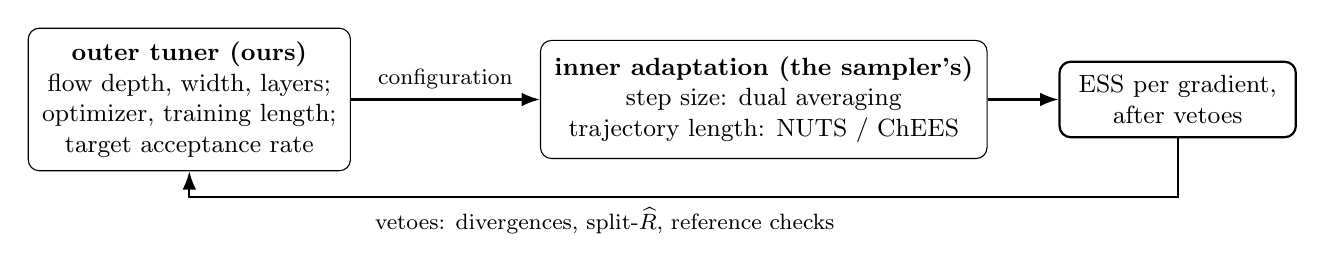
\begin{tikzpicture}[
  box/.style={draw, rounded corners, align=center, inner sep=5pt, font=\small},
  arr/.style={-{Latex}, thick},
  node distance=8mm and 24mm]
\node[box, minimum width=40mm, minimum height=15mm] (outer)
  {\textbf{outer tuner (ours)}\\flow depth, width, layers;\\optimizer, training length;\\target acceptance rate};
\node[box, right=of outer, minimum width=52mm, minimum height=15mm] (inner)
  {\textbf{inner adaptation (the sampler's)}\\step size: dual averaging\\trajectory length: NUTS / ChEES};
\draw[arr] (outer.east) -- node[above, font=\footnotesize] {configuration} (inner.west);
\draw[arr] (inner.east) -- ++(0.9,0) node[right, box, minimum width=30mm, align=center] (score)
  {ESS per gradient,\\after vetoes};
\draw[arr] (score.south) |- ++(-2.0,-0.75) -| node[below, pos=0.25, font=\footnotesize]
  {vetoes: divergences, split-$\widehat{R}$, reference checks} (outer.south);
\end{tikzpicture}
\caption{The two tuning loops of a neural-transport sampler. The inner
adapters already solve step size and trajectory length; the outer tuner
owns what they cannot reach, and its objective is efficiency (effective
samples per gradient) gated by correctness vetoes that no efficiency
score can buy off.}
\label{fig:sampler-loops}
\end{figure}

The outer objective already has a citable template, and it is the NeuTra
paper's own. Its authors selected step size and leapfrog steps by
Bayesian optimization on an objective that rewards effective sample size
(ESS, the number of independent draws a correlated chain is worth)
per gradient evaluation while sharply penalizing configurations whose
potential-scale-reduction diagnostic $\widehat{R}$ departs from one
\citep{hoffman2019neutra}; tuning samplers by BO goes back at least to
\citet{mahendran2012adaptive}. Effective samples per gradient is the
right currency because gradient evaluations dominate cost in both flow
training and leapfrog integration.

But ESS estimated from short chains
is exactly the kind of proxy that Chapter~\ref{sec:multifidelity} warned
about, and sampler tuning has a sharper failure mode than slow starters:
a chain that mixes quickly inside one mode of a multimodal posterior
reports excellent short-run ESS while being wrong, the statistical
equivalent of Figure~\ref{fig:curves}'s sprinter, except that this
sprinter never stalls visibly; it simply reports the wrong answer with
growing confidence.

The remedy is to treat correctness diagnostics as
vetoes rather than objectives: divergence counts, split $\widehat{R}$
across independent chains, and, where a reference posterior is available
on a pilot problem, agreement with it. A configuration that fails a veto
is discarded no matter how efficient it looks; among configurations that
pass, ESS per gradient is a legitimate objective. Multi-fidelity
structure is still available (shorter chains, fewer chains), but rung
promotion should require the vetoes to pass at every rung, which is
exactly the kind of user-defined gate our scheduler interfaces must
support (Chapter~\ref{sec:architecture}).

The concrete default: a single-objective study on ESS per gradient with
divergence and split-$\widehat{R}$ vetoes at every rung, ASHA over chain
length as the scheduler, the GP searcher of Chapter~\ref{sec:bayesian}
over the flow and training knobs, and the inner adapters left switched
on with only their target acceptance rate exposed to the search.

\section{Hamiltonian and physics-structured networks}

Hamiltonian neural networks learn a scalar function whose symplectic
gradient supplies the dynamics; conservation comes from the architecture
rather than from a penalty term, and the original paper reports models
that conserve an energy-like quantity where an unconstrained baseline
drifts \citep{greydanus2019hnn}. Notably for us, its authors chose their
hyperparameters by a coarse grid over learning rate, layer width,
activation, and batch size, which is precisely the procedure
Chapter~\ref{sec:modelfree} retired; the field's own tuning practice
trails its modeling practice, and that gap is our opportunity.

Tuning these models well is multi-objective in the evaluation even when
the training loss is a single term: short-horizon prediction error,
long-rollout state error, and energy drift move separately, the training
loss sees only the first, and the scientific value lives in the second
and third.

The axes of Figure~\ref{fig:pareto} were chosen with this
workload in mind, and the study template is the one that figure
illustrates: a two-or-three-objective search (prediction error,
long-rollout error or energy drift, optionally training cost) solved
with qLogNEHVI or MO-ASHA from Chapter~\ref{sec:moo}, over a space that
includes integrator choice and step size, width and depth, activation
(smoothness matters when the learned function is differentiated),
learning rate, and loss weights where present. Where variants do carry
multi-term losses (the pixel-observation task in the original paper
combines the dynamics loss with autoencoder terms), the weights joining
them are exactly the knobs an outer tuner should own.

Trials are cheap,
minutes rather than hours, so this is also the workload where the
tuner's own overhead (Section~\ref{sec:costmodel}) is most visible and
the local execution backend of Chapter~\ref{sec:architecture} earns its
keep.

A neighboring literature balances competing loss terms inside training
rather than outside it: gradient-statistics reweighting for
physics-informed networks \citep{wang2020pathologies}, weights set
from neural-tangent-kernel eigenvalues \citep{wang2020ntk}, and relative
loss balancing schemes compared systematically by
\citet{bischof2025relobralo}. The division-of-labor rule from the
sampler subsection transfers unchanged: where internal balancing works,
let the trainer balance and let the tuner search what the trainer
cannot, and when in doubt, the internal balancer is a competitor our
outer loop must beat at matched cost, not a rival to ignore.

\section{Architecture search, in moderation}

Our NAS folder is full of ambitious methods, and the sober reading of the
field is that a small team should adopt its cheap findings and skip its
expensive machinery. The thousand-paper survey of \citet{white2023nas1000}
recommends random search as the mandatory baseline for any NAS claim
(Chapter~\ref{sec:modelfree}'s discipline, enforced field-wide) and
records that simple quantities such as parameter count and FLOPs
(floating-point operation counts) are
surprisingly competitive with the leading zero-cost proxies, whose
reliability degrades on larger search spaces. Systematic bench-marking of
those proxies found their value to lie in complementing a learned
performance predictor rather than in standalone selection
\citep{krishnakumar2022nasbenchsuite}.

On the one-shot side, the DARTS
family is documented to produce degenerate architectures across a range
of search spaces without careful regularization \citep{zela2020robustifying},
and controlled evaluations found much of the reported progress
attributable to training tricks rather than to the search itself, with
hand-designed macro-structure mattering more than the searched cells
\citep{yang2020frustratingly}.

Meanwhile the benchmark built for joint
architecture-and-hyperparameter search motivates itself with the
observation that good hyperparameters can matter more than the best
architecture \citep{bansal2022jahs}.

For us, the conclusion is comfortable: architecture search should mean
width, depth, and a few structural flags included as ordinal and
categorical axes in the ordinary search space (as BG-PBT does for policy
and value networks, with the ordinal-aware kernels of
Section~\ref{sec:highdim} doing the modeling), multi-fidelity doing the
heavy lifting, parameter count reported as an objective when size
matters, and no dedicated weight-sharing subsystem. That covers every
architecture question our current projects actually ask, at a small
fraction of the complexity.

Because ``in moderation'' is the kind of phrase that drifts, the
boundary is worth stating as a scope rather than as a mood. Inside it:
width and depth as ordinal axes, a small number of structural flags
(normalization choice, residual connections, activation family) as
categorical axes, parameter count and measured FLOPs available as
objectives for the multi-objective machinery of
Chapter~\ref{sec:moo} rather than as proxies substituting for
training, and architecture coordinates mutating through the same
explore step every other coordinate uses, which is what BG-PBT's
architecture handling amounts to once the weight-sharing is stripped
out (Chapter~\ref{sec:population}). Outside it, deliberately: topology
and cell search, one-shot or weight-sharing supernets, a zero-cost
proxy subsystem, grammar-based or hierarchical architecture spaces
\citep{schrodi2023grammar}, and differentiable search of any flavor.
The exclusions are not a claim that those methods fail; they are the
claim this chapter's evidence actually supports, which is that they
cost a subsystem each and buy nothing our workloads have asked for. A
project that needs them needs a different governing document, and the
honest move then is to write one rather than to widen this sentence.

One consequence is worth flagging where it lands. Changing width or
depth mid-run invalidates the weights a population method wants to
inherit, so a population arm that mutates an architecture coordinate
pays for the change: either it restarts the trial from initialization,
or it transfers what it can by distillation from the parent, which is
the route BG-PBT takes \citep{wan2022bgpbt} and which
Chapter~\ref{sec:population} treats as part of the population line's
price rather than as free.

\section{The compute bill, and the shortcuts we are asked about}
\label{sec:computebill}

Tuning reinforcement learning is expensive enough that the fair question
is not ``which method'' but ``can we afford any of this,'' so the bill
deserves to be written out. A study's cost factors cleanly into three
multiplied terms: the number of candidate configurations examined, times
the seeds per candidate that Chapter~\ref{sec:workloads}'s protocol
demands, times the training steps per trial. In the running example the
last factor alone is up to 150 million environment steps, hours on
several accelerators, so a naive 64-candidate, 3-seed, full-length study
is roughly two hundred full training runs before anything has been
learned about tuning at all.

Every lever this document recommends
attacks one factor: multi-fidelity scheduling cuts steps per trial by
an order of magnitude (Chapter~\ref{sec:multifidelity}, and it is the
biggest single lever); model-based search and warm starts cut the
number of candidates (Chapters~\ref{sec:bayesian}
and~\ref{sec:transfer}); the seed protocol stops compute being spent
optimizing luck; population methods make the trials \emph{be} the
training run rather than a rehearsal for it
(Chapter~\ref{sec:population}); and ARLBench-style representative
benchmark subsets cut the cost of evaluating tuner changes by roughly
an order of magnitude \citep{becktepe2024arlbench}, which is what makes
our own validation suite affordable.

Against that backdrop, three architecture-search shortcuts come up
whenever the bill is discussed, and each deserves a plain description
and a verdict.

\emph{One-shot search} trains a single ``supernet'' that contains every
candidate architecture as a sub-network with shared weights; candidates
are then scored by inheriting weights from the supernet instead of being
trained separately, so one big training run amortizes thousands of
evaluations. The economics are attractive and the evidence is not. The
DARTS family of one-shot methods is documented to produce degenerate
architectures across search spaces without careful regularization
\citep{zela2020robustifying}; controlled re-evaluations attribute much
of the reported progress to training tricks rather than the search, with
hand-designed macro-structure mattering more than the searched cells
\citep{yang2020frustratingly}; and the field's own thousand-paper survey
responds by making random search the mandatory baseline
\citep{white2023nas1000}.

Two further points are specific to us rather
than to the literature, and we label them as our inference: supernet
training assumes a stable supervised training signal, while RL's data
distribution shifts under the policy as it learns; and our architecture
questions concern small policy and value networks, where there is not
enough training to amortize for the supernet's economy to pay. Verdict:
no one-shot subsystem, for reliability reasons first and fit reasons
second.

\emph{Zero-shot search} (zero-cost proxies) scores architectures at
initialization, without any training, from quantities like gradient
statistics at the first batch; the promise is architecture selection
for the price of a forward-backward pass. The systematic benchmark of
these proxies found their value to lie in complementing a learned
performance predictor rather than in standalone selection, with
reliability degrading on larger spaces
\citep{krishnakumar2022nasbenchsuite}, and the survey notes that plain
parameter count and FLOPs are surprisingly competitive with the
sophisticated proxies \citep{white2023nas1000}. That last fact is the
actionable one: params and FLOPs are free, we already record them in
the run store, and they can serve as objectives or tie-breakers today.
Verdict: report the free quantities; build no proxy subsystem.

\emph{Grammar-based spaces} attack a different problem than cost.
A context-free grammar generates architectures the way a grammar
generates sentences: production rules expand high-level structure into
blocks and blocks into operations, which compactly defines hierarchical
search spaces vastly larger than the usual cell catalogs, searched with
Bayesian optimization over hierarchical kernels
\citep{schrodi2023grammar}; NePS ships support for such spaces
(Chapter~\ref{sec:libraries}). The honest reading for a manager: this
is a solution to \emph{expressiveness}, letting one search whole
macro-structures rather than a fixed menu, and a larger space raises
rather than lowers the number of evaluations needed. It becomes
relevant the day a project genuinely needs to discover topology; every
architecture question our projects ask today is width, depth, and
flags, where the benchmark evidence says hyperparameters matter at
least as much as the architecture anyway \citep{bansal2022jahs}.
Verdict: not in the package now; NePS is the reference implementation
if a topology-search project ever lands.

The summary sentence for the section: the compute problem in RL tuning
is real, and its solution in our package is the stack of levers in the
first paragraph, not an architecture-search shortcut; the shortcuts
either lack reliability evidence (one-shot), reduce to free quantities
we already record (zero-shot), or solve a problem we do not have
(grammar spaces).

\begin{decisions}
\noindent\textbf{Decisions from this chapter.} Per workload, the study
we configure today; and the architecture-search verdicts.
\begin{itemize}[leftmargin=1.3em, itemsep=2pt]
\item \textbf{RL, routine budgets} (a few dozen full runs): DEHB or
BO-plus-ASHA over the full plausible space, several tuning seeds,
disjoint test seeds, objective recorded explicitly. \textbf{RL, large
parallelism} (8+ workers): the population line, PB2-Mix now, BG-PBT
when built.
\item \textbf{Neural-transport samplers}: GP searcher over flow and
training knobs, ASHA over chain length, ESS-per-gradient objective,
divergence and split-$\widehat{R}$ vetoes at every rung; leave the
samplers' internal adapters on.
\item \textbf{Hamiltonian networks}: two-to-three-objective study
(prediction error, energy drift or rollout error, optionally cost)
with qLogNEHVI or MO-ASHA, on the local execution backend.
\item \textbf{Architecture search}: width, depth, and flags as
ordinary search axes; parameter count and FLOPs reported as free
objectives. \textbf{One-shot supernets}: exclude (reliability evidence
against, RL mismatch). \textbf{Zero-cost proxy subsystem}: exclude
(free quantities capture most of the value). \textbf{Grammar-based
spaces}: exclude for now (solves expressiveness, not cost; no current
project needs topology discovery); NePS is the reference if that
changes.
\end{itemize}
\end{decisions}

\section{What would overturn these verdicts}

The routine-budget RL verdict (DEHB or BO+ASHA) is decided by V07;
whichever loses is excluded and this section rewritten. The sampler
study's veto gates are tied to V13: if vetoes prove unreliable
(failing configurations promoted, or survivors ranking poorly
against the reference posterior), correctness checking is pulled
back into training code and the tuner's veto hook is disabled. The
Hamiltonian study's reliance on the premium MO searcher follows
V09's outcome; if qLogNEHVI is demoted, the study defaults to
scalarization. The workload-template abstraction itself (four
matched studies, not a general tuner) holds unless colleagues
request a fifth workload family with evidence that it differs
structurally from the four, at which point a new template is argued
and added or the request is accommodated by parameterizing an
existing one.

\chapter{The open-source libraries, one by one}
\label{sec:libraries}

The method chapters told us what is worth running; this one asks who
actually ships it, and in what condition. Every version number,
maintenance signal, and feature claim in this chapter was checked against
the project's own repository, package index, release notes, or
documentation on August 22, 2026, and re-checked on August 23; the
summary appears in Table~\ref{tab:libraries}. Maintenance status is a fact with a date on it,
not a permanent verdict, and it matters here as much as algorithmic content:
several famous names below are no longer safe foundations. A useful way to
read the section is to sort the field by what each project fundamentally is:
a few are \emph{execution frameworks} that run and schedule trials, most are
\emph{search engines} that propose configurations and expect someone else to
run them, and two are \emph{services} wrapping a search engine behind a
network API. Our product needs exactly one good member of the first kind and
a curated set of the second.

\section{Execution frameworks}

\paragraph{Ray Tune.}
Part of Ray (release 2.57.0, August 11, 2026, Apache 2.0), Tune runs
distributed trials natively on a Ray cluster, with fault tolerance and a
stable Tuner interface. Its scheduler side is genuinely strong: ASHA,
Hyperband, median stopping, a BOHB scheduler, and the only mainstream
native distributed implementations of population-based training, PBT with
replay, and PB2, with the documented requirement that the trainable
support checkpoint save and restore \citep{liaw2018tune, moritz2018ray}.
Two findings from the release history temper the picture. First, across
the five Ray releases from December 2025 to August 2026, every
Tune-specific change was a documentation restructure, example, or bug fix;
no new algorithm or capability landed in that window. Second, the roster
of bundled search integrations has been deliberately pruned: Dragonfly,
SigOpt, scikit-optimize, and FLAML's searchers are gone from the current
documentation, leaving wrappers for Ax, bayesian-optimization, BOHB (whose
upstream is unmaintained, see below), HEBO, Hyperopt, Nevergrad, Optuna,
and ZOOpt. Core Tune has no native multi-objective support: the tuner
takes one metric and one mode, and Pareto workloads pass through the
Optuna searcher, which accepts lists of metrics. The fair summary: a
first-class execution and scheduling substrate whose own search
intelligence is coasting, which is precisely the shape of dependency we
want underneath a search layer of our own.

\paragraph{Syne Tune.}
Originally from AWS, now in its own community organization (release
0.16.0, August 3, 2026, Apache 2.0, about 420 GitHub stars), Syne Tune is
the closest existing thing to the product this document proposes: a broad
method zoo (multi-fidelity, multi-objective, transfer, and
population-based training all claimed in its README) behind a backend
abstraction that can execute trials locally, on SageMaker, or inside a
simulator that replays tabular and surrogate benchmarks faster than real
time \citep{salinas2022synetune}. That simulator is unique in the field
and exactly the right idea for cheap algorithm regression tests. The
concerns are social rather than technical: a small community and a
post-corporate maintenance arrangement, with no Ray backend, so adopting
it as our substrate would mean owning a second execution stack beside the
one RLlib already requires. We take its backend-abstraction design and its
simulator idea as blueprints rather than its code as foundation.

\paragraph{Katib.}
Kubeflow's Kubernetes-native tuner (v0.19.0, October 2025, Apache 2.0)
runs trials as Kubernetes workloads defined by custom resources, with
early stopping and a set of suggestion services that mostly wrap Optuna,
Goptuna, and Hyperopt. It is the right shape for an organization whose
platform is Kubeflow; on a Ray shop it duplicates the execution layer we
already have while adding no search capability we could not get from the
wrapped engines directly.

\paragraph{Determined and NNI.}
Two cautionary entries. Determined, the training platform whose adaptive
ASHA implementation was well regarded, has had no repository activity
since March 2025 and no release since then either, without any formal
notice; do not build on it. NNI, Microsoft's once-popular AutoML toolkit,
is formally archived (last release September 2023), and its fourteen
thousand GitHub stars are a trap for anyone ranking libraries by
popularity.

\section{Search engines}

\paragraph{Optuna.}
Optuna (4.9.0 in June 2026, 5.0 release candidate in August 2026, MIT) is
where sampler development is most active in 2026
\citep{akiba2019optuna}. The 5.0 line promotes a multivariate TPE with a
constant-liar strategy for parallel workers to the default sampler;
recent 4.x releases grew the GP sampler into constrained and
multi-objective territory (a log-EHVI acquisition, plus batch-proposal
strategies), an automatic sampler-selection module ships through the
OptunaHub plugin registry, and a Rust core accelerates the standard
samplers. Its define-by-run interface remains the best available way to
express conditional search spaces, and NSGA-II is the default for
multi-objective studies, with the multi-objective TPE variant
\citep{ozaki2020motpe} now folded into the standard sampler rather than
shipped separately. The limitation is the mirror image of Ray
Tune's: Optuna executes nothing. Its documented multi-node story is a
relational database that workers poll, with an explicit warning about
file-based storage over NFS, and it has no population-based training.
Optuna behind Ray Tune's OptunaSearch is the pairing both projects
document, and it is the pairing new tools reach for: DataRobot's syftr,
an agent-workflow optimizer released in 2025, states in its README that
it builds on Ray for distributed execution and Optuna for
define-by-run search and multi-objective optimization.

\paragraph{Ax and BoTorch.}
Meta's pair covers the model-based frontier: BoTorch (0.18.1, June 2026,
MIT) supplies the Gaussian-process machinery and the modern acquisition
functions, including the qLogNEHVI family that Chapter~\ref{sec:moo}
recommends, and its own documentation warns users off the older
non-log variants; Ax (1.3.1, June 2026, MIT) wraps it in a clean ask-tell
client aimed at practitioners, defaulting to noisy expected hypervolume
improvement for multi-objective studies
\citep{balandat2020botorch}. BoTorch's README is candid that end users
not doing BO research should use Ax instead. Neither executes trials;
both are exactly the acquisition engine our GP searchers should be built
on rather than reimplemented.

\paragraph{SMAC3.}
The AutoML group's random-forest Bayesian optimizer (2.4.0, April 2026,
BSD) remains actively developed, with multi-fidelity and multi-objective
support across its facades and a 2.4.0 change of default surrogate to
scikit-learn's random forest \citep{lindauer2022smac3}. It is the
canonical engine for large conditional spaces and the tuner used as the
sequential baseline in the BG-PBT paper. Its ergonomics are single-machine
and academic; we would wrap it for awkward spaces rather than adopt its
frame.

\paragraph{NePS.}
Neural Pipeline Search from the same group (0.16.0, March 2026, Apache
2.0, under a hundred stars but actively developed) is the reference home
of the prior-and-multi-fidelity methods we care about: PriorBand, ifBO,
and a multi-objective variant with expert priors, plus grammar-based
hierarchical architecture spaces. Its parallelism model is workers
coordinating through a shared results directory, simple and DDP-friendly,
though the same design that Optuna's documentation warns can race over
NFS. For us it is a source of reference implementations and a
correctness oracle for our own PriorBand and ifBO ports, not a substrate.

\paragraph{DEHB and HpBandSter.}
The two AutoML-group bandit engines are both frozen, in different ways.
DEHB (0.1.2, mid 2024) announces in its README that it is maintained for
stability but no longer actively developed; the algorithm remains the
evidence-backed recommendation for small-budget RL tuning
(Chapter~\ref{sec:workloads}), so the pragmatic path is to implement DEHB
against our own interfaces with the frozen package as a reference.
HpBandSter, the reference BOHB implementation, opens its README with
``not maintained anymore''; notably, Ray Tune's BOHB searcher still
depends on it.

\paragraph{Hyperopt, Nevergrad, FLAML.}
Hyperopt (0.3.0, July 2026) received its first release since 2021, a
compatibility revival with no new methods; it matters today mainly as the
legacy TPE many codebases still import. Nevergrad (1.0.12, April 2025,
sixteen months without a release at our check date) remains a broad
evolutionary toolbox whose NGOpt wizard picks among CMA-ES, differential
evolution, and dozens of other solvers by problem features; a good
non-BO baseline for bake-offs. FLAML (2.6.0, April 2026, active) is the
cost-frugal specialist: its CFO and BlendSearch searchers start cheap and
spend more only when justified, with explicit fields for the cost-related
hyperparameters \citep{wang2021flaml}; its Ray integration, however, has
disappeared from Ray's documentation, so using it means wiring it
ourselves.

\paragraph{OpenBox.}
An academic black-box optimization service (0.9.0, March 2026, MIT) with
an unusually broad claim sheet: multi-objective, constraints, transfer,
early stopping, and a REST service mode \citep{li2021openbox}. Activity
is modest and burst-like, and the service architecture duplicates
infrastructure a Ray shop already runs. Worth watching, not depending on.

\section{Services and partial offerings}

\paragraph{Open-source Vizier.}
Google's Vizier (client-server, Apache 2.0) publishes the most complete
description of an industrial default anywhere: a Mat\'ern-5/2 GP with
MAP-fit hyperparameters, an output-warping stack that tames outliers, a
deliberately explorative UCB coefficient, trust regions, and an
evolutionary acquisition maximizer, benchmarked in its own report against
algorithms accessed through Ray Tune \citep{song2022ossvizier,
song2024vizier}. The repository is active but the package on PyPI had not
been released for eighteen months at our check date. Its value to us is
the design disclosure more than the dependency.

\paragraph{Weights and Biases sweeps.}
The open pieces are the client and a small suggestion library (random,
grid, a Bayesian sampler, Hyperband stopping) whose standalone package
last shipped in 2022; orchestration and state live in the proprietary
service. Fine as a convenience for W\&B customers; not an engine to build
on.

\paragraph{New arrivals worth a footnote.}
The visible new energy of 2025 and 2026 sits in agentic tooling rather
than classical search: an official Optuna server exposing studies to
language-model agents, and a fast-growing project that has coding agents
iterate on training configurations directly. None of these publish
controlled evidence against the methods of
Chapters~\ref{sec:bayesian}--\ref{sec:transfer} at matched budgets, so
they change nothing in our plan, but they are worth rechecking in a year.

\begin{table}[t]
\centering
\small
\caption{Open-source tuning libraries as checked on August 22, 2026.
``Maintained'' reflects release and commit activity at that date, not a
prediction. Stars are approximate GitHub counts.}
\label{tab:libraries}
\begin{tabular}{@{}llll@{}}
\toprule
Library & Release (date) & Status & One-line reading \\
\midrule
Ray Tune & Ray 2.57.0 (2026-08) & active; Tune coasting & best executor; search layer aging \\
Optuna & 4.9.0; 5.0rc1 (2026-08) & very active & best samplers; no executor \\
Ax & 1.3.1 (2026-06) & active & polished BO client over BoTorch \\
BoTorch & 0.18.1 (2026-06) & active & the acquisition engine to reuse \\
Syne Tune & 0.16.0 (2026-08) & active, small team & broadest methods; design blueprint \\
SMAC3 & 2.4.0 (2026-04) & active & conditional-space BO plus racing \\
NePS & 0.16.0 (2026-03) & active, small team & PriorBand and ifBO reference code \\
DEHB & 0.1.2 (2024-07) & stability-only & algorithm good; package frozen \\
HpBandSter & 0.7.4 (2018-11) & unmaintained & BOHB reference; do not depend \\
Hyperopt & 0.3.0 (2026-07) & compatibility only & legacy TPE \\
Nevergrad & 1.0.12 (2025-04) & slowing & evolutionary baseline (NGOpt) \\
FLAML & 2.6.0 (2026-04) & active & cost-frugal searchers \\
OpenBox & 0.9.0 (2026-03) & sporadic & broad claims, small team \\
OSS Vizier & 0.1.24 (2025-02) & repo active, releases stalled & reference design disclosure \\
Katib & 0.19.0 (2025-10) & active & Kubernetes-native; redundant on Ray \\
Determined & 0.38.1 (2025-03) & dormant & no activity since early 2025 \\
NNI & 3.0 (2023-09) & archived & formally retired \\
Orion & 0.2.7 (2023-03) & dormant & no release in over three years \\
W\&B sweeps & lib 0.2.0 (2022-08) & minimal open core & orchestration is proprietary \\
\bottomrule
\end{tabular}
\end{table}


\part{The product proposal}
\chapter{The product, concretely}
\label{sec:product}

Everything before this page weighed evidence; this part spends it. The
reader changes here too: the chapters so far served whoever must judge
our verdicts, and the chapters from here serve whoever must build from
them, starting the week the plan is approved. The two jobs meet in one
requirement, so we state it before any design.

\emph{Concrete} has a checkable meaning in this part, and it is not
``more detail.'' A verdict from the decision boxes counts as delivered
only when four anchors exist for it: a contract (which interface,
schema, or component carries it), a test (which entry of the
validation suite would catch its failure), a schedule slot (which tier
and week builds it), and a price (whose weeks pay for it). The master
table of Chapter~\ref{sec:roadmap} already lists every verdict with
its tier and cost; this part's job is to supply the two missing
anchors, contracts and tests, and to close the loop so that no
verdict lives only in a box.

The part runs in build order. This chapter says what the product is
and walks one study through it on day one.
Chapter~\ref{sec:architecture} holds the architectural design, two
interfaces, two adapters, and a database, unchanged from the verdict
it argued. The chapters after it pin the contracts and the validation
suite, and Chapter~\ref{sec:roadmap} closes the part with the
schedule and the bill.

\section{What we ship, and to whom}

The product is an internal Python package: a tuning layer that our
four workload families call, running on Ray Tune as its execution
layer, exactly as Chapter~\ref{sec:architecture} argues. It is not a
service, not a platform, and not a research program; every research
bet it contains (the learning-curve scheduler, the population
flagship) is scheduled behind a working default, not in front of it.

The customers are the projects of Chapter~\ref{sec:workloads}, and
the package meets each one with a configured study rather than a menu:
the routine-budget RL study, the large-parallelism RL study, the
sampler study with its correctness vetoes, and the two-objective
Hamiltonian study. A researcher who knows only their own workload
should be able to run the matching study without reading this part
of the document; the chapters exist so that the person
\emph{extending} the package can reconstruct why each default is what
it is.

What ships, in one sentence per layer: a search-space schema that
knows the three knob kinds, conditional structure, and an optional
prior; a searcher interface and a scheduler interface with wrapped
implementations behind them (Optuna's TPE and the GP searcher on one
side, ASHA and the median rule on the other); a run store that
records configurations, seeds, curves, costs, and lineage; the seed
protocol as the default study shape rather than an option; and the
validation suite, which is a deliverable of the same rank as the
tuner, because every falsification promise made in
Chapters~\ref{sec:modelfree} through~\ref{sec:transfer} is an entry
in it.

\section{A study on day one}

The fastest way to make the product concrete is to run one study
through it in words, at tier~0, using only components that exist and
are maintained today plus our thin glue. Nothing in this walk waits
on research; that is what ``wire up what exists'' meant in
Chapter~\ref{sec:roadmap}, and the walk doubles as the acceptance
test for tier~0.

A researcher opens a study for the running example: PPO on the Brax
task, routine budget, the situation of Chapter~\ref{sec:workloads}.
They declare the fifteen-knob space of Chapter~\ref{sec:problem} in the
schema, unchanged and with no knob added: learning rate log-uniform
between $10^{-5}$ and $10^{-2}$, the ordinal widths, depths, and batch
sizes as ordered integers, and the two spectral-normalization flags as
categories. The BG-PBT space carries no conditional knob, so this study
declares a flat space; the schema's conditional support is exercised by
the annealing switch of Chapter~\ref{sec:problem} and by the off-policy
and sampler workloads of Chapter~\ref{sec:workloads}, and the
capability test for it lives there rather than here. The schema also
accepts the folklore prior (learning rate
near $3 \times 10^{-4}$, discount near $0.99$) as a first-class
field. On day one nothing consumes it; recording it from day one is
deliberate, because Chapter~\ref{sec:transfer} showed that priors
are cheap to store, expensive to retrofit, and eventually worth
real trials.

They declare the objective explicitly, mean evaluated return aggregated
over the declared tuning seeds, because Chapter~\ref{sec:workloads}
showed that final return, area under the curve, and truncated return
genuinely disagree, and a hidden default here silently changes every
ranking downstream. This tuning-seed mean is what the searcher observes
and optimizes. After selection is frozen, the winner (or Pareto front)
is evaluated once on disjoint test seeds that the tuner never saw, and
that held-out performance is what the final report quotes.

This seed protocol is the study's default shape: search driven by
tuning-seed feedback, final evaluation on test seeds. This is not an
option the researcher enables; it is the study shape, and opting
\emph{out} is the act that requires writing something down. The
evidence for that inversion is the seed-noise record of
Chapters~\ref{sec:problem} and~\ref{sec:workloads}, and the protocol
is what makes the test set a genuine held-out evaluation rather than
part of the search feedback loop.

The searcher on day one is the wrapped TPE; the scheduler is ASHA
with the median rule beside it, granting first rungs at one tenth of
full fidelity. While the study runs, every trial streams its curve
into the run store with its configuration, seed, rung history, and
bill, and the store computes one diagnostic the researcher did not
ask for: the rank correlation between rung scores and final scores,
logged per study. That number is Chapter~\ref{sec:multifidelity}'s
crossing-curves hazard turned into a measured quantity of our own
workloads, and the validation suite consumes it later.

What the researcher gets back is the incumbent configuration with
its test-seed mean and spread, the full record of trials in the
store, and the study's own audit trail: which trials were stopped at
which rungs, and what the early-versus-final correlation was. What
they do not get on day one, stated as plainly: no schedules (the
population line is tier~2), no premium multi-objective searcher (the
Hamiltonian study runs on the wrapped evolutionary default until the
qLogNEHVI searcher lands), and no prior-weighted acquisition yet.
Each absence has a tier and a week in Chapter~\ref{sec:roadmap};
none of them blocks the day-one study from being useful, which is
the point of the tier ordering.

\section{The register, and how this part uses it}

Chapter~\ref{sec:roadmap}'s Table~\ref{tab:decisions} is the spine
of this part: every verdict, its tier, its cost, and the chapter
holding its evidence. The two chapters that follow extend each row
with its remaining anchors. The contracts chapter names the
interface or schema field that carries the verdict, so that a reader
can point from ``priors are first-class'' to the line of the schema
that makes it true. The validation chapter names the suite entry
that would catch the verdict failing, and it inherits its content
from promises already made: every ``argued from four angles''
section in Chapters~\ref{sec:modelfree}
through~\ref{sec:transfer} ended with a falsification criterion, and
the suite is those criteria collected, priced, and scheduled rather
than restated.

Two bookkeeping rules keep the register honest while this part is
written. A verdict with no plausible suite entry is marked
untestable in place, with a sentence saying why, rather than
receiving a decorative test. And any design sentence in this part
that cannot cite a chapter of evidence is labeled an engineering
judgment, so the reader always knows which statements the survey
backs and which ones the build team owns.

\section{What would overturn this chapter}

The day-one walk is this chapter's load-bearing claim: tier~0 is
composition, not construction. It fails, and this part gets
rewritten, if the walk cannot be reproduced in software within the
tier~0 budget of Chapter~\ref{sec:roadmap}, if any step turns out to
require a component the audit of Chapter~\ref{sec:libraries} did not
verify as maintained, or if the seed-protocol default proves too
expensive to be the default on our routine studies. The first
validation-suite run is scheduled to test exactly this walk, and the
suite, not this chapter, has the last word.

\chapter{Is Ray Tune the right base, and what we should build on it}
\label{sec:architecture}

The question that started this document can now be answered with the
evidence laid out. Yes, Ray Tune is the right base, provided we are clear
about which layer of the problem it solves. Tune should run our trials; it
should not choose them. The search intelligence, which is where the field
has moved fastest and where Tune has moved least, belongs in a layer we
own. This chapter turns that sentence into a design, and the design is
small: the whole proposal is two interfaces, two adapters, and a database.

\section{The case for Tune underneath}

Three facts carry the decision. First, we already operate Ray: RLlib
training runs on the same cluster, speaks the same actor model, and
produces the checkpoints that population-based methods need to copy and
resume. A second execution stack would be pure overhead. Second, Tune's
execution machinery is the strongest available in open source for our
shape of work: multi-node trial scheduling, fault tolerance,
checkpoint-aware schedulers, and the only mainstream native distributed
PBT and PB2 (Chapter~\ref{sec:libraries}). The population family of
Chapter~\ref{sec:population} is the part of our roadmap with the most
demanding executor requirements, exploit steps are checkpoint surgery
performed live on a running population, and Tune is the one framework
that has already productionized them. Third, the composition we propose
is the one the ecosystem itself converges on: Optuna and Ray document
each other as the intended pairing, a 2025 industrial optimizer built
its stack exactly this way, and Google's published account of its own
tuning service benchmarks against algorithms accessed through Ray Tune
\citep{song2024vizier}.

The risks deserve equal daylight, and Chapter~\ref{sec:libraries}
documented them with dates. Tune's own search layer has been coasting:
across the five Ray releases from late 2025 through August 2026, every
Tune change was a fix or a documentation edit, several of its remaining
searcher integrations wrap upstreams that are frozen or formally
unmaintained, and core Tune still has no native concept of a Pareto
front, which after Chapter~\ref{sec:moo} we regard as a first-class
requirement rather than a nicety. None of this argues against Tune as an
executor; all of it argues against depending on Tune for algorithms.
There is also a real overhead concern at the small end: for the cheap
trials of our Hamiltonian-network work
(Section~\ref{sec:costmodel}), cluster machinery can cost more than the
training it schedules.

\section{The design}

The consequence is a three-layer design, drawn in
Figure~\ref{fig:architecture}. At the top, a search layer that is the
actual product: searchers (ask-and-tell proposers: GP with qLogEI and
qLogNEHVI on BoTorch, TPE via Optuna, CMA-ES, the mixed-space
trust-region searcher that BG-PBT needs) and schedulers (ASHA and the
median rule, their multi-objective variants with veto gates, the
population controllers), all written against two small interfaces of our
own. The split between the two interfaces is exactly the split drawn in
Figure~\ref{fig:loop} at the start of the document: searchers answer
``which configuration next,'' schedulers answer ``how much budget, and
does this trial live''; every method surveyed decomposes into the two
roles, and keeping the roles separate is what lets ASHA schedule trials
proposed by any searcher.

In the middle, thin adapters: one maps our interfaces onto Ray Tune's
searcher and trial-scheduler protocols and is the default; one runs
trials in local processes for laptop-scale studies where Ray does not
earn its overhead; the design leaves room for a queue-based backend
later, following the backend abstraction that Syne Tune demonstrated
\citep{salinas2022synetune}. At the bottom, alongside the executors, a
run store that records every trial of every study: configuration, seeds,
fidelity-indexed curves, cost, diagnostics, and lineage (which weights
were copied from whom, for population methods). The store is what turns
the transfer methods of Chapter~\ref{sec:transfer} from papers into
features, warm starts are a query against it, and $\pi$BO priors and
fitted cost models are trained from it, and it is also where a study's
evidence lives when we later ask whether the tuner is earning its keep.

To make the layering concrete, walk one trial of the running example
through it. The GP searcher (top layer) proposes a configuration by
maximizing qLogEI over the mixed space; the MO-ASHA scheduler assigns it
a rung-1 budget of two million steps. The Ray adapter translates both
decisions into a Tune trial with a checkpoint interval; RLlib trains it
on the cluster and streams evaluation returns back. At the rung
boundary the scheduler ranks the rung (non-dominated sorting if the
study is multi-objective), checks the trial's veto fields, and either
promotes it, at which point the adapter resumes it from its checkpoint,
or stops it. Every intermediate return, the cost, the seed, and the
promotion decision land in the run store. Nothing in the top layer knows
Ray exists; nothing below the adapters knows what an acquisition
function is. That ignorance is the design.

Owning the two interfaces, rather than coding directly against Tune's, is
what keeps the Tune risks bounded. If Tune stagnates further or Ray's
APIs shift again, the adapters change and the product does not. It is
also what lets the same searcher serve both executors, so a Hamiltonian
study on a workstation and a PPO population on the cluster run the same
code paths above the adapter line.

Three features must be first-class in those interfaces because
retrofitting them is painful, and each traces to a specific finding
earlier in the document. Multiple objectives and constraint vetoes: a
scheduler must be able to rank partial results by non-dominated sorting
and to refuse promotion to a trial that failed a correctness diagnostic,
whatever its score; this is the promotion machinery of
Chapter~\ref{sec:moo} and the veto gates that
Figure~\ref{fig:sampler-loops} showed the sampler workload demanding.
Seeds: a trial is a configuration times a seed, aggregation across seeds
is the tuner's job, and tuning seeds are disjoint from test seeds by
construction, the protocol whose absence corrupted the RL results
surveyed in Chapter~\ref{sec:workloads}
\citep{eimer2023hyperparameters}. Schedules: the outcome of a population
study is a trajectory with lineage, storable and replayable, the bold
path of Figure~\ref{fig:pbt} as a first-class object (Tune's own
PBT-replay scheduler shows the shape).

\begin{figure}[t]
\centering
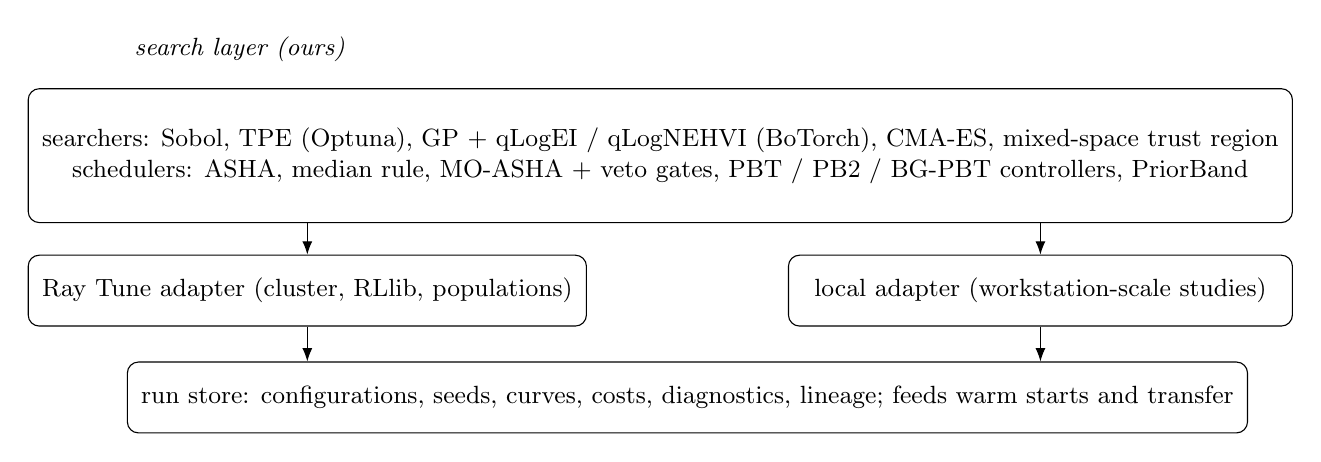
\begin{tikzpicture}[
  box/.style={draw, rounded corners, align=center, inner sep=5pt, font=\small},
  lab/.style={font=\small\itshape, anchor=west},
  node distance=4mm and 5mm]
\node[box, minimum width=136mm, minimum height=17mm] (search) at (0,0)
  {searchers: Sobol, TPE (Optuna), GP + qLogEI / qLogNEHVI (BoTorch), CMA-ES, mixed-space trust region\\
   schedulers: ASHA, median rule, MO-ASHA + veto gates, PBT / PB2 / BG-PBT controllers, PriorBand};
\node[lab] at (-6.8,1.35) {search layer (ours)};
\node[box, minimum width=64mm, minimum height=9mm, below=of search.south west, anchor=north west, xshift=0mm] (ray)
  {Ray Tune adapter (cluster, RLlib, populations)};
\node[box, minimum width=64mm, minimum height=9mm, below=of search.south east, anchor=north east] (local)
  {local adapter (workstation-scale studies)};
\node[box, minimum width=136mm, minimum height=9mm] (store) at ($(ray.south east)!0.5!(local.south west)$) [yshift=-9mm]
  {run store: configurations, seeds, curves, costs, diagnostics, lineage; feeds warm starts and transfer};
\draw[-{Latex}] (search.south -| ray) -- (ray.north);
\draw[-{Latex}] (search.south -| local) -- (local.north);
\draw[-{Latex}] (ray.south) -- (ray.south |- store.north);
\draw[-{Latex}] (local.south) -- (local.south |- store.north);
\end{tikzpicture}
\caption{The proposed layering. Algorithms live above the adapter line
and survive any change of executor; Ray Tune supplies distributed
execution and checkpoint surgery; a shared run store accumulates the
evidence that priors, warm starts, and transfer methods consume. The
two interfaces at the adapter line are the searcher/scheduler split of
Figure~\ref{fig:loop}, made contractual.}
\label{fig:architecture}
\end{figure}

\section{Alternatives we considered}

Adopting Syne Tune outright would buy the broadest method zoo in one
package, and its simulator backend is a genuinely good idea we intend to
copy; against that stand a small maintainer base, no Ray backend, and a
method set that still lacks the BG-PBT-class population line we care
about.

Building on Optuna alone would give us the best samplers and
nothing to run them with: its documented multi-node story is a shared
relational database, and there is no population machinery. NePS has the
freshest prior-and-fidelity algorithms and we will use it as a reference
implementation and correctness oracle, but its filesystem coordination
and small community rule it out as a substrate.

Katib solves execution
for Kubernetes shops; we are a Ray shop. Writing our own executor from
scratch is the option nobody should pick while Tune exists and is
maintained. The remaining risk in our choice is Ray itself drifting in a
direction that breaks Tune; the adapter boundary is the insurance, and
the annual cost of that insurance is two small interfaces.

\chapter{Interfaces and data contracts}
\label{sec:contracts}

Chapter~\ref{sec:architecture} argued that the whole proposal is two
interfaces, two adapters, and a database. This chapter makes those
five things exact enough to code against. The discipline throughout:
every field and every method either names the verdict it carries,
with the chapter holding the evidence, or is labeled an engineering
judgment that the build team owns. A reader should be able to point
from any line of the eventual code review back to a line of this
survey, or know that no such line exists.

One vocabulary note before the details. A \emph{study} is the unit a
researcher opens: one search space, one objective declaration, one
budget, many trials. The contracts below are organized the way a
study meets them: first what the researcher declares, then the two
decision-makers (searcher and scheduler), then the store that
remembers everything, then the executors that pay the bills.

\section{The study declaration}

A study begins with a declaration, and the declaration is where
several chapters' verdicts become unavoidable rather than optional.

The \emph{objective declaration} names the quantity being optimized,
its direction, and its evaluation protocol. For RL studies that means
choosing among final evaluated return, area under the training curve,
and return at a fixed budget, explicitly, because
Chapter~\ref{sec:workloads} showed the three orderings genuinely
disagree; the field is mandatory and recorded, never defaulted
silently. Multi-objective studies declare a vector of such
objectives, and the product treats the front as the study's output
from that moment (Chapter~\ref{sec:moo}).

The \emph{seed protocol} is part of the declaration, with defaults
rather than blanks: a number of tuning seeds per candidate and a
disjoint set of test seeds for the final report, the protocol of
\citet{eimer2023hyperparameters} that Chapters~\ref{sec:problem}
and~\ref{sec:workloads} adopted. Opting out is possible and is
itself recorded, so a study that skipped the protocol says so in its
own audit trail.

The \emph{budget declaration} states the study's size in full-run
equivalents and the number of concurrently available full-length
workers. The second number exists because of
Chapter~\ref{sec:population}'s boundary: at eight or more dedicated
workers with a schedule-shaped question the population line becomes
eligible, and below it the product steers to the rung methods. The
declaration is what lets the product enforce that boundary in
software rather than trusting each user's optimism.

\section{The search-space schema}

The schema is a tree of knob declarations, one per hyperparameter,
and its fields track exactly the structure
Chapter~\ref{sec:problem} taught.

\begin{description}[style=nextline, leftmargin=1.6em, itemsep=2pt]
\item[kind] One of continuous, ordinal, categorical. Three values,
not the four kinds of Chapter~\ref{sec:problem}, because the fourth
is structural rather than typed: a conditional knob is a continuous,
ordinal, or categorical knob that also carries a predicate, so
conditionality lives in \textbf{condition} below. Integer-valued
knobs are ordinals, the ordinal kind being defined as an integer with
a natural order, and there is no separate integer kind to choose. The
distinction that remains
is load-bearing downstream: ordinals are modeled as ordered, never as
unordered labels, because respecting the order produced measurable
gains in the BG-PBT ablations (Chapter~\ref{sec:bayesian},
Section~\ref{sec:highdim}), and categorical axes route to overlap
kernels or per-category machinery rather than being embedded and
hoped about.
\item[range and transform] Bounds for continuous and ordinal knobs,
the value list for categorical ones, and an optional transform, with
log-uniform as the expected choice for scale-type knobs; the 90
percent of a uniform draw wasted in the top decade
(Chapter~\ref{sec:modelfree}) is the argument, and the same flag
drives input warping in the GP searcher.
\item[condition] An optional parent-knob-and-value predicate. A
conditional knob exists only when its predicate holds, which makes
the space a tree rather than a box; TPE consumes this natively, and
searchers that cannot must say so through their capability flags
below rather than silently sampling meaningless coordinates
(Chapters~\ref{sec:problem} and~\ref{sec:bayesian}).
\item[prior] An optional distribution over the knob, the expert's
belief about where the optimum lies. First-class from day one
because retrofitting it is expensive and every project lead has one
(Chapter~\ref{sec:transfer}); consumed by the $\pi$BO weight and the
PriorBand portfolio once tier~1 lands, recorded but inert before
that.
\item[note] Free text for units and meaning. An engineering judgment
with a purpose: the schema doubles as the study's documentation, and
Chapter~\ref{sec:problem}'s knob tour is the register this field is
meant to echo.
\end{description}

\section{The searcher interface}

A searcher proposes configurations and learns from results. The
interface is deliberately small.

\begin{description}[style=nextline, leftmargin=1.6em, itemsep=2pt]
\item[propose(n, state)] Return $n$ configurations to evaluate next.
Batch proposals are the normal case, not the extension, because idle
workers were Chapter~\ref{sec:bayesian}'s standing argument; a GP
searcher implements $n > 1$ by joint batch acquisition and handles
still-running trials by fantasies, exactly the machinery of
Section~\ref{sec:acquisition}.
\item[observe(record)] Ingest one trial record from the store,
including partial-fidelity observations; a searcher that only
understands final scores declares that limitation.
\item[capabilities] A static declaration: which knob kinds, whether
conditionals are supported, whether multiple objectives are, whether
a prior is consumed, maximum sensible dimension. The product refuses
a mismatched study loudly at declaration time. The flag exists
because the audit of Chapter~\ref{sec:libraries} found exactly such
mismatches shipping silently (a continuous-only PB2 is the standing
example), and refusing early is cheaper than diagnosing a silently
degenerate study.
\item[snapshot and restore] Serialize internal state, so long
studies survive restarts and population methods can fork searcher
state along a lineage. Engineering judgment on the mechanism; the
requirement itself follows from the population line's design
(Chapter~\ref{sec:population}).
\end{description}

Behind this interface, tier~0 ships wrapped implementations (Optuna
TPE, the BoTorch GP with qLogEI and dimension-scaled priors, CMA-ES,
Sobol and log-uniform random), tier~1 adds qLogNEHVI, Chebyshev
scalarization, the $\pi$BO weight, and EI-per-cost as decorators on
the GP searcher, and the trust-region mixed-space searcher arrives as
the shared core of high-dimensional single-objective search and the
population line's explore step (Chapters~\ref{sec:bayesian}
and~\ref{sec:population}).

\section{The scheduler interface}

A scheduler allocates budget across running trials. Its contract has
one more verb than the classical statement, because the population
line needs it.

\begin{description}[style=nextline, leftmargin=1.6em, itemsep=2pt]
\item[report(trial, fidelity, value)] Called as metrics stream in;
returns continue, stop, or pause. ASHA and the median rule live
entirely behind this verb, which is why they ask nothing of training
code beyond streaming a metric (Chapter~\ref{sec:multifidelity}).
\item[promote()] Return paused or new trials to run when a worker
frees, with rung bookkeeping ($\eta$, initial budget $r$) internal
to the scheduler. Asynchronous promotion against results-so-far is
the ASHA rule; a PASHA flag stops growing the top rung once
rankings stabilize.
\item[gate(predicate)] Register a veto evaluated at every rung. A
trial failing its gate is discarded regardless of its score; this is
the sampler workload's divergence and split-$\widehat{R}$ machinery
generalized into a hook (Chapter~\ref{sec:workloads}), and MO-ASHA's
correctness gates use the same mechanism (Chapter~\ref{sec:moo}).
\item[exploit(loser, winner) and explore(config)] The population
verbs: copy weights and hyperparameters from winner to loser through
the executor's checkpoint surgery, then perturb or re-propose via a
searcher. Keeping these on the scheduler interface, with the
searcher consulted for explore, is precisely the entanglement
Chapter~\ref{sec:population} described, made explicit instead of
implicit.
\end{description}

Every scheduler decision lands in the store with its reason, because
the audit trail is a product feature, not a log file: the researcher
of Chapter~\ref{sec:product}'s walk reads exactly this record.

\section{The run store}

The store is one database with three kinds of rows, and several
chapters' promises are really promises about these rows.

Trial rows carry the configuration, seed, rung history with
per-rung scores and costs, the full learning curve, final objective
values as a vector, veto outcomes, and a parent-trial pointer. The
parent pointer is the population line's lineage: with it, a
hyperparameter \emph{schedule} is a walk up the tree, queryable
after the study, which is what ``schedules are a first-class
output'' meant concretely in Chapter~\ref{sec:population}.

Study rows carry the declaration in full (space, objective, seeds,
budget, boundary inputs), the incumbent or front over time, and the
study-level diagnostics, of which one is computed always: the rank
correlation between rung scores and final scores.
Chapter~\ref{sec:multifidelity} promised that the crossing-curves
hazard would become a measured property of our workloads; this row
is where the measurement lives, and the validation suite consumes
it.

Query surfaces are part of the contract because two verdicts depend
on them: warm starting a new study from configurations that ranked
well on similar past studies (Chapter~\ref{sec:transfer}) is a
ranked query over trial rows, and hypervolume-over-budget reporting
(Chapter~\ref{sec:roadmap}) is a scan over study rows. Storage
technology is an engineering judgment; the schema above is not.

\section{The executor adapters}

Two adapters, per the architecture chapter. The Ray Tune adapter
maps trials to Tune trials and must expose checkpoint surgery as
first-class operations: save, copy weights and optimizer state
across trials, resume. That is the machinery PBT exercises inside
Tune today and the single strongest reason
Chapter~\ref{sec:architecture} kept Tune underneath; our adapter's
job is to keep it reachable from the scheduler's exploit verb. The
local adapter runs minutes-scale trials in-process for the
Hamiltonian regime, where Chapter~\ref{sec:workloads} showed the
distributed stack's overhead is the visible cost. Both adapters
meter per-trial cost themselves, because EI-per-cost consumes
measured cost, not the user's folklore (Chapter~\ref{sec:transfer}).

\section{The architecture factory}
\label{sec:archfactory}

One contract exists only because Chapter~\ref{sec:workloads} decided
that architecture search means width, depth, and a few structural
flags rather than topology. Those coordinates sit in the ordinary
search space, so the searcher and scheduler interfaces above need no
new verbs for them; what they do need is a way to turn a
configuration into a model, and a way to say when two configurations'
models can share weights. Both belong to the user's workload, not to
the tuner, which is why they are a contract rather than an
implementation.

\begin{description}[style=nextline, leftmargin=1.6em, itemsep=2pt]
\item[build(config)] Return an initialized model from the
architecture coordinates of a configuration. The workload supplies
this; the product never constructs architectures itself, because the
space of things a user might mean by ``depth'' is not ours to
enumerate. The factory is also what makes the excluded methods
excluded by construction: a contract that maps coordinates to a model
has no place to put a supernet.
\item[measure(model)] Return the size objectives, parameter count and
FLOPs per forward pass, for a built model. These are measured on the
constructed model rather than predicted from the coordinates, which
is the whole reason Chapter~\ref{sec:workloads} was willing to treat
size as an objective and unwilling to treat proxies as a substitute
for training. Multi-objective studies consume these through the
ordinary objective vector (Chapter~\ref{sec:moo}).
\item[compatible(config$_a$, config$_b$)] Declare whether weights
from one configuration's model can be loaded into another's. Pure
hyperparameter changes are compatible; a width or depth change is
not. The scheduler's exploit verb consults this before checkpoint
surgery, and an incompatible answer routes the trial to the transfer
policy below instead of copying weights into a shape that cannot hold
them. A workload that gets this predicate wrong produces silent
garbage, so the conformance suite tests it directly: every declared
compatible pair must survive a load, and every incompatible pair must
refuse one.
\item[transfer(parent, child)] The policy for an incompatible
inheritance: restart the child from initialization, or warm-start it
by distillation from the parent, which is BG-PBT's route
(Chapter~\ref{sec:population}). The choice is declared per study, not
inferred, and its cost is charged to the trial that caused it rather
than hidden in the population's overhead. Distillation arrives with
the population line in tier~2; before then the only legal policy is
restart, and the factory says so through its capability flags.
\end{description}

The searcher's \textbf{capabilities} declaration gains one flag to
match: whether the searcher models architecture coordinates as
ordinals and categoricals with the rest of the space, or requires
them held fixed. A searcher answering the latter is not eligible for
a study whose space includes architecture axes, and the product
refuses the combination at declaration time for the same reason it
refuses a continuous-only searcher on a categorical space.

\section{What would overturn this chapter}

Contracts are falsified by construction work, and the suite is
arranged to do it early: if the tier~0 wraps cannot be expressed
behind these interfaces without holes, if the reference-parity tests
of Chapter~\ref{sec:validation} need interface changes to pass, or
if the population verbs prove insufficient for a faithful PBT run
on the Ray adapter, the contracts change and this chapter is
rewritten before the code doubles down. The interfaces are the
product's most expensive thing to change later; that is why they
get a chapter, a register mapping, and the first weeks of the
calendar rather than an afternoon.

\chapter{The validation suite}
\label{sec:validation}

A tuning product can fool its builders the same way a configuration
fools a tuner: by being evaluated on the problems it was tuned on.
This document has met the trap twice, as seed overfitting in
Chapter~\ref{sec:workloads} and as the proxy bias of
Figure~\ref{fig:curves}, and the defense is the same both times:
decide the evaluation before the thing being evaluated exists. This
chapter is that decision. It collects every falsification promise
made in Chapters~\ref{sec:modelfree} through~\ref{sec:product} into
numbered tests with pass rules, prices the expensive ones, and ties
each build tier's completion to named entries rather than to the
feeling of being done.

\section{Three layers}

The suite runs at three costs, and a test's layer is part of its
identity.

Layer one is cheap and broad: surrogate and tabular benchmarks
(YAHPO-Gym, HPOBench, and the RL-specific ARLBench), where a full
tuner comparison costs CPU-minutes because the training runs were
paid for once by others \citep{pfisterer2022yahpo,
eggensperger2021hpobench, becktepe2024arlbench}, plus recorded-curve
replays in the style of Syne Tune's simulator
(Chapter~\ref{sec:libraries}), where a scheduler's decisions are
re-executed against stored learning curves in seconds. A scheduler
bug found in a CPU-minute replay is a bug not found in a GPU-week
study; layer one exists to make that sentence routine. The
multi-fidelity-with-priors suite from the PriorBand line covers the
prior-handling code specifically \citep{mallik2023priorband}.

Layer two is realistic and ours: one pinned task per workload
family. A PPO task on a Brax environment; a flow-plus-HMC sampler
task scored by ESS per gradient under divergence and
split-$\widehat{R}$ vetoes, with a reference posterior computed once
at great length; a Hamiltonian network task scored on prediction
error and energy drift. Layer two is where verdicts about \emph{our}
workloads are settled, at GPU prices, under the statistical
discipline of Section~\ref{sec:val-protocol}.

Layer three is standing: diagnostics that run inside every real
study the product ever executes. The rank correlation between rung
scores and final scores is logged always
(Chapter~\ref{sec:multifidelity}); the seed protocol's presence or
explicitly recorded absence is part of every study row
(Chapter~\ref{sec:contracts}). Layer three is how the suite keeps
learning after release, and it costs nothing because the store
records it anyway.

\section{The register of tests}

Table~\ref{tab:suite} is the register. Each entry names the claim
under test, the protocol in one line, the rule that passes or vetoes,
the chapter whose promise it discharges, and the tier gate it
belongs to. The subsections after it expand the entries whose
protocols need more than a line.

\begin{table}[tp]
\centering
\footnotesize
\renewcommand{\arraystretch}{0.95}
\caption{The validation register. Layer 1 runs on tabular benchmarks
and replays (CPU); layer 2 on the pinned tasks (GPU); layer 3 inside
every production study. ``Gate'' names the tier that cannot be
declared done until the entry is green.}
\label{tab:suite}
\begin{tabularx}{\textwidth}{@{}l>{\raggedright\arraybackslash}X>{\raggedright\arraybackslash}Xll@{}}
\toprule
ID & Claim under test & Pass rule or veto & Evid. & Gate \\
\midrule
V01 & each wrapped searcher/scheduler matches its reference
implementation on tabular benchmarks & final and anytime scores
within tolerance of reference & \ref{sec:libraries} & T0 \\
V02 & scheduler logic is correct under asynchrony & replayed
decisions on recorded curves match specification; stragglers and
drops simulated & \ref{sec:multifidelity} & T0 \\
V03 & the suite itself catches wiring bugs & seeded defects
(off-by-one rung, dropped seed, swapped objective sign) are caught
by V01--V02 & \ref{sec:product} & T0 \\
V04 & every shipped searcher earns its complexity & beats the
log+Sobol floor at matched budget on pinned tasks, each searcher
tested at the gate of the tier that ships it: the tier-0 GP with
qLogEI and the wrapped TPE at the tier-0 gate, the tier-1 and later
searchers at theirs & \ref{sec:modelfree}, \ref{sec:bayesian} &
T0/T1 \\
V05 & the transform matters as claimed & GP with and without
log-warping on a pinned task; warped must not lose & \ref{sec:modelfree} & T0 \\
V06 & early stopping is nearly free & searcher+ASHA matches
searcher-at-full-fidelity final quality within noise at a fraction
of compute; rung correlations logged & \ref{sec:multifidelity} & T1 \\
V07 & the small-budget RL verdict holds here & DEHB vs BO+ASHA at
matched 16-run budget on the pinned RL task & \ref{sec:multifidelity},
\ref{sec:population} & T3 \\
V08 & the population line does not lose in its home regime & population line vs
DEHB and BO+ASHA on both sides of the eight-worker line at matched
compute; 3 reps/arm/side (declared exception,
Sec.~\ref{sec:val-v08}); consistent home loss demotes the flagship,
disagreement reports unresolved & \ref{sec:population} & T2 \\
V09 & the premium MO searcher earns its tier & qLogNEHVI vs
random-weight Chebyshev and wrapped NSGA-II on the Hamiltonian task;
hypervolume with uncertainty; demote to option on a tie & \ref{sec:moo} & T1 \\
V10 & cheap MO fidelity signals may cull & short-horizon drift
passes the rank-correlation pilot before MO-ASHA may kill on it & \ref{sec:moo} & T1 \\
V11 & priors are safe to default-on & no-prior vs folklore-prior vs
wrong-prior runs; gains under good, recovery within noise under
wrong, else demote to opt-in & \ref{sec:transfer} & T1 \\
V12 & warm starts pay & measured trial savings on a new study of a
familiar family once the store holds enough studies & \ref{sec:transfer} & T1$^{+}$ \\
V13 & sampler correctness cannot be bought by speed & veto-failing
configurations never promoted; survivors ranked by ESS/gradient;
pilot agreement with the reference posterior & \ref{sec:workloads} & T1 \\
V14 & tier 0 is composition, not construction & the day-one walk of
Chapter~\ref{sec:product} reproduced end to end within the tier-0
budget & \ref{sec:product} & T0 \\
V15 & the curve-model bet is live before we pay for it & ifBO
matches or beats ASHA on the curve-informative public suites before
any integration work & \ref{sec:multifidelity} & T3 \\
\bottomrule
\end{tabularx}
\end{table}

\section{The statistical protocol}
\label{sec:val-protocol}

Every layer-two comparison follows one protocol, copied from the
discipline of \citet{eimer2023hyperparameters} and from this
document's own warnings. Fixed tuning seeds and disjoint test seeds.
Budgets matched on measured cost, with the tuner's own overhead
included in the bill. Results reported as performance-over-budget
curves with uncertainty bands, never as single numbers. And a
repetition count that is derived rather than declared: a pilot
campaign estimates the between-run variance, and the sample size
follows from that variance and the entry's decision margin at 80
percent power. The ten repetitions this document has quoted since
Chapter~\ref{sec:workloads} are a planning heuristic for the
calendar and the budget, not a substitute for that calculation.
Where the pilot shows low variance against a wide margin, fewer
repetitions suffice and the protocol records why; where it shows
high variance against a narrow one, the budget rises or the claim
softens, and the entry says which.

Because the budget is finite, every entry also carries a maximum
sample size, and reaching it without crossing the decision threshold
is a third outcome alongside pass and fail: \emph{inconclusive at
budgeted precision}. That is a real verdict with a real consequence,
which is that the capability does not become a default on evidence
that never arrived. Pilot variance estimates are recorded before the
full campaign begins and are not revised during it, since a variance
estimate updated mid-campaign is a decision threshold updated
mid-campaign wearing a disguise. V08 remains the one entry whose arms
are too expensive for any of this at full strength; it runs three
repetitions per arm per side under the restricted question,
asymmetric demotion rule, and release semantics of
Section~\ref{sec:val-v08}, and any future exception is written into
this section before its campaign runs, never after its results are
seen.

Verdicts then come in three strengths, and the suite's reports use
the distinction explicitly. Hard vetoes (a diverged run promoted, a
veto-failing configuration surviving, a protected seed leaking into
tuning) fail a test regardless of scores. Descriptive differences
(one curve above another within overlapping bands) are recorded and
never rank anything. A ranking is claimed only when the repetitions
support it statistically; when a result shows one method ahead
within noise, the honest summary is that they tied, and a tie
against a simpler method is a loss for the complex one wherever the
register says so (V04, V09). The suite exists to catch regressions
and to rank where gaps are real, not to manufacture leaderboard
drama.

\subsection{Register shorthand resolved}

The table above uses unquantified phrases to fit on one page; this
section pins each one to a concrete rule before any entry runs.

\textbf{``Within tolerance'' (V01):} Anytime and final scores differ
by no more than $0.5\%$ of the reference method's final value on each
benchmark, and rank orderings match exactly. The tolerance is loose
by design—V01 gates implementation correctness, not optimizer
superiority.

\textbf{``Within noise'' (V06, V11):} The 95\% bootstrap confidence
interval of the difference in means lies entirely inside the
preregistered non-inferiority margin $[-\delta, +\delta]$: for V06,
$\delta$ is 5 percent of the full-fidelity baseline's final quality;
for V11, 10 percent of the no-prior baseline's. Bootstrap by
resampling tuning runs with replacement, 10,000 iterations,
empirical percentiles. The distinction from an interval that merely
overlaps zero is the whole point. Overlapping zero says a difference
was not detected, which a small enough sample says about everything;
an interval contained in the margin says any difference that
survives is too small to care about. An interval that overlaps zero
but spills past $\pm\delta$ is recorded as inconclusive, not as a
tie, and a tie is claimed only in the contained case. Both margins
are set here, before the campaigns, as the smallest difference that
would change what the product recommends.

\textbf{``A fraction of compute'' (V06):} Early stopping reaches the
same final quality, within the non-inferiority margin above, at no
more than one-third the total compute of full-fidelity search.
Compute is the accelerator-seconds and wall-clock the executor
actually recorded, which puts startup, training, evaluation,
checkpoint save and load, queue wait, and the optimizer's own
overhead on the bill; the savings claim is about resources consumed,
not about an idealization of them. Full-run equivalents survive as a
normalized secondary measure for readability, computed by dividing
total cost by the mean cost of one full-fidelity trial in the
baseline arm, and they are never the number the gate reads. The
threshold applies to accelerator-seconds. Where wall-clock diverges
materially from it through scheduling or parallelism, both are
reported and the verdict follows the accelerator-seconds, since that
is the resource the budget buys. V06 passes only if ASHA delivers the
factor-of-three saving on measured cost.

\textbf{``Measured trial savings'' (V12):} The warm-started study
reaches the same final objective value in at least 20\% fewer trials
than a cold start on the same task. Both arms use the same searcher;
only the initialization differs. Below 20\%, warm starting is not
worth defaulting on.

\textbf{``Hypervolume with uncertainty'' (V09):} Report hypervolume
over budget with 95\% confidence bands from bootstrap resampling of
tuning runs. Rank methods by their final hypervolume; demote the
premium method (qLogNEHVI) to an option if the interval overlaps the
simpler method's (Chebyshev) or if it loses outright.

\textbf{``Enough studies'' (V12):} The run store must contain at
least ten completed studies from the same model family (same
architecture class, same task domain) before V12 runs. Below that,
the warm-start query has no data to learn from and the test is
meaningless.

All numerical gates (0.5\%, one-third, 20\%, 0.6 for V10, 1.01 for
V13) are judgments recorded before the data arrives, not fit to
results. The V10 and V13 protocols later in this chapter set their
thresholds explicitly; the phrases above inherit the same discipline.

\subsection{Sampling levels and paired designs}

A tuning comparison has more than one source of randomness, and
conflating them is the fastest way to a confident wrong answer. Five
levels are in play: the optimizer seed (which tuning run), the
workload training seed (which initialization or environment
instance), the evaluation seed (which test episodes), the task
(which benchmark), and the configuration draw (which candidates the
searcher happened to try). Treating the leaves as independent samples
when the branches are shared is pseudoreplication: it shrinks the
reported interval without adding information, and every gate
downstream inherits the false precision.

The first defense is pairing. Where a comparison admits it, the
methods share the optimizer seed set, the task and environment
instances, and any baseline configurations drawn once and evaluated
by all arms. Pairing removes the between-instance variance from the
contrast rather than averaging over it, which buys power at no extra
compute, and it applies wherever the methods being compared consume
seeds the same way. Where they do not, because a population method
spends seeds on a schedule a sequential method has no analogue for,
the entry says so and falls back to unpaired sampling with the larger
sample size the power calculation then demands.

Uncertainty is computed by hierarchical bootstrap rather than by
resampling individual trials. The resampling unit is the complete
tuning run; when runs span several tasks, tasks are resampled and
then runs within the sampled tasks, preserving the nesting. The
statistic of interest is recomputed on each of 10,000 bootstrap
samples and reported at empirical percentiles. This propagates every
level's variance without assuming a distributional form for any of
them, and it is the procedure behind every interval quoted in this
chapter.

\subsection{Development and acceptance tasks}

The trap this chapter opened with applies to the suite itself. A
pinned task that implementers run daily while debugging stops being a
held-out measurement of anything; it becomes the thing the
implementation was tuned on, and the gate it anchors measures fit to
the validation set. So each workload family carries two disjoint task
sets. Development tasks are named in week one of tier~0, recorded in
the validation manifest, and free to run as often as anyone likes.
Acceptance tasks are chosen by an engineer not implementing the
capability under test, revealed at gate time, and recorded in the
gate manifest with their data checksums.

Both numbers are reported, and the gap between them is itself a
diagnostic: a capability strong on development tasks and weak on
acceptance tasks has overfit the suite, which is a finding rather
than a mystery. Promotion decisions weigh the acceptance results,
because those are the only ones the implementation has not seen.

Task sets rotate on a version, not on a feeling. When a tier's gates
are recorded, new tasks enter development and some older development
tasks may migrate to acceptance for the next tier, with version
numbers and dates in the task registry. The registry is what makes
task-selection bias auditable after the fact, which matters
precisely because the person selecting is usually the person hoping.

\subsection{Multiple comparisons and endpoints}

Several entries ask more than one question. V04 compares searchers
across tasks and budget points; V09 crosses objectives with
comparators; V13 inspects many posterior marginals at once. Twenty
independent comparisons at the conventional threshold produce one
spurious winner on average, which is enough to promote a searcher
that does nothing.

Each entry therefore predeclares one primary endpoint, the single
comparison the tier's completion depends on, and labels the rest.
The primary endpoint is judged at $\alpha = 0.05$ uncorrected,
because there is one of it. Secondary comparisons that feed a ranking
claim are controlled family-wise at $\alpha = 0.05$ by the
Holm--Bonferroni stepdown procedure \citep{holm1979simple}, which is
uniformly more powerful than plain Bonferroni at the same guarantee
and needs no assumption about dependence among the tests.
Comparisons that rank nothing and decide nothing, the descriptive
kind this chapter has already licensed, need no correction, and
saying so is what keeps multiplicity control from becoming a tax on
honest reporting.

V04's primary endpoint, as the worked instance: whether the tier-0 GP
with qLogEI beats the log-plus-Sobol floor on the acceptance task at
matched budget. Comparisons among GP variants, or across development
tasks, are secondary and corrected. Every entry's primary endpoint is
written into its protocol before its campaign begins, for the same
reason its thresholds are.

\subsection{Immutable artifacts and preregistration}

None of the above binds unless the plan provably predates the data,
so every gate campaign emits a signed manifest before it runs. The
manifest is JSON and carries the protocol version and entry
identifier (\texttt{V04-T0-v1.2} and the like), SHA-256 checksums of
task code, data files, and environment configuration, the exact
tuning and test seed sets per method and repetition, the analysis
script with its thresholds and tests committed to version control
while the results do not yet exist, a full dependency lock and
hardware description, the commit hash of the code under test, and a
creation timestamp with a signature.

Results are written as versioned JSON with the manifest hash
embedded, under \texttt{validation/artifacts/}, a path deliberately
not ignored by \texttt{.gitignore}. Reanalysis is permitted and
expected; what it may not do is quietly replace the first analysis. A
changed threshold, a changed script, or a changed seed set after
results are visible produces a new manifest at an incremented version
with the reason written down, and both versions survive.

The point is not ceremony. Researcher degrees of freedom
\citep{simmons2011false} are invisible in a report and obvious in a
diff, and this is the cheapest available way to put them in a diff: a
reviewer can check that the analysis plan predates the data, that the
tested code matches the history, and that the tasks and seeds were
not chosen after the fact to flatter a result the team had already
grown attached to.

\section{The two expensive campaigns}
\label{sec:val-v08}

Two entries dominate the compute bill and deserve their design
stated in advance.

V07 races DEHB against BO+ASHA at a matched sixteen-full-run budget
on the pinned RL task, ten repetitions each. The cost driver is the
pinned task's full-run price, so the task is sized in week one with
ARLBench's guidance on representative subsets, which cut tuner
evaluation cost by roughly an order of magnitude in their study
\citep{becktepe2024arlbench}. As a sizing illustration, labeled an
estimate: if one full run costs two accelerator-hours on the chosen
environment, the campaign is $2 \times 16 \times 10 \times 2 = 640$
accelerator-hours, under a month on a single dedicated node and a
weekend on eight. If the chosen environment cannot fit that
envelope, the environment is wrong, not the protocol.

V08 is the flagship's trial, run late, when the population line
exists: the population method against DEHB and BO+ASHA on both sides
of the eight-worker boundary at matched total compute. It is the one
entry where the ten-repetition rule collides with the price of the
test, because a single population arm already costs eight
full-length trainings, and ten repetitions on both sides of the
boundary is a quarter-million accelerator-hour campaign we will not
buy. The exception is therefore stated as a protocol rather than
waved through. The repetition count drops to three per arm per side,
the smallest number that still yields a spread rather than a point,
and the reduction is paid for by narrowing the question: V08 does not
ask which method is best, only whether the boundary sits where
Chapter~\ref{sec:population} says it does. Three arms, two sides,
three repetitions, and the ordering of arms within a side is what the
entry reports, with the observed spread shown always.

The stopping rule is written in advance, because a cheap test with a
flexible endpoint is worse than no test. If all three repetitions on
a side agree in ordering, the side is called and no further
repetitions are bought. If they disagree, the entry reports
\emph{unresolved at this budget} and the flagship keeps whatever
status it had going in, which is a hold rather than a promotion; the
one outcome V08 may never produce is a promotion on evidence that did
not separate. The demotion direction is asymmetric and deliberately
so: a consistent loss in the flagship's home regime demotes it on
three repetitions, because the claim being falsified is a strong one
and a strong claim can be broken by a weak test, whereas confirming
the boundary would need the full protocol we declined to buy. That
asymmetry is the honest content of a three-repetition campaign, and
it is why V08 is written here as a falsifier of
Chapter~\ref{sec:population}'s threshold rather than as its
validation.

The result states and their release consequences are named too, since
a falsifier with no defined pass state cannot gate a tier. V08 opens
at \emph{hold: insufficient evidence} and can reach three places.
\emph{Demote}: all three repetitions on a side agree that the
population line loses in its home regime, in which case the flagship
becomes an experimental option and the roadmap's defaults revert to
whichever of DEHB or BO+ASHA won V07. \emph{Hold}: the repetitions
disagree, or the home-regime side is inconclusive, in which case the
entry stays at \emph{unresolved at this budget} and the flagship
keeps its tier-2 experimental status without becoming a default
recommendation. \emph{Pass}: reachable only through the full
sequential campaign this entry declined to buy, at up to ten
repetitions per arm per side with preregistered margins and decision
boundaries. The three-repetition run is a tripwire, not promotion
evidence, and no accumulation of tripwires becomes one.

Tier~2 completion therefore requires that V08 be neither demoted nor
blocked by an implementation failure; a hold is acceptable
completion. That is the honest reading of a capability whose audience
is users at eight or more dedicated workers: the population line
ships as an option with Chapter~\ref{sec:population}'s boundary
documented as guidance rather than enforced as a default, and the
campaign that would promote it waits for tier~3 or a post-release
cycle, if demand and budget ever arrive together.

\section{Two entries whose protocol needs pinning}

V10 and V13 both gate a capability on a threshold, so the threshold
has to be a number chosen before the data arrives rather than after.

V10 asks whether a short-horizon energy-drift measurement may cull a
Hamiltonian trial. The pilot runs a fixed set of one hundred
configurations drawn uniformly from the search space, each at a
single fixed seed, to full fidelity (the study's declared endpoint),
recording drift at the candidate rung (proposed as one third of the
endpoint) and at the end. The gate metric is Spearman rank
correlation between the two drift vectors (one value per
configuration, not per run, since single-seed eliminates within-config
variance). Compute the bootstrap 95\% confidence interval by
resampling configurations with replacement 10,000 times and taking
empirical percentiles of the resampled correlations. MO-ASHA may kill
on that signal only if the interval's lower bound clears $0.6$. Below
it, the scheduler still runs but the signal is advisory, promotion
decisions falling back to the objective that does correlate. The
number 0.6 is a judgment, not a result from the literature, and it is
recorded here so that a later argument about it is an argument about
a written-down choice. The hundred-trial campaign costs about 133
full runs on the Hamiltonian task, budgeted under layer-two
validation.

V13 asks whether the sampler study's correctness vetoes hold. Three
components, each with its own rule. The vetoes themselves are
absolute: any configuration with a divergent transition or
split-$\widehat{R}$ above $1.01$ is never promoted, and a single
promotion of a veto-failing configuration fails the entry outright.
The sampling protocol that feeds the vetoes: four independent chains
per configuration, each from a dispersed random initialization, 2,000
warmup draws discarded plus 2,000 retained draws per chain, for 8,000
posterior samples total per configuration. Split-$\widehat{R}$ is
computed by splitting each chain in half (eight half-chains) and
comparing within-half-chain variance to between-half-chain variance
per the rank-normalized folded formula of \citet{vehtari2021rhat}; the
veto fires if any marginal exceeds $1.01$ or if effective sample size
falls below 400. Divergent transitions are reported by the sampler
itself (a numerical-integration failure during the Hamiltonian
trajectory). A bimodal or multimodal target is detected by visual
inspection of marginal trace plots during the pilot; if found, chains
are re-initialized from dispersed modes rather than randomly, per
Bayesian workflow recommendations.

Survivors are ranked by effective sample size per gradient evaluation,
the cost measure the executor records rather than one the user
supplies. And agreement with the reference posterior is checked on the
pilot: the reference is computed once at great length using the same
four-chain protocol but with 20,000 retained draws per chain, and each
candidate configuration's marginal means and variances are compared to
the reference marginals. Agreement is defined as: the candidate's
posterior mean falls within one standard error of the reference
posterior mean, where the standard error of each mean is $\sigma /
\sqrt{\text{ESS}}$, using each sampler's own reported effective sample
size and posterior standard deviation. An entry that ranks a fast,
subtly wrong sampler above a slow, correct one is the failure this
test exists to catch, which is why speed enters only after the vetoes
and the agreement check have passed.

\section{Sabotage entries}

Two entries test the testers. V03 seeds defects into the wiring, an
off-by-one rung, a dropped seed, a flipped objective sign, and
requires the parity and replay layers to catch them; a suite that
cannot catch a planted bug is decoration, and this entry is the
reason we can trust green elsewhere. V11 seeds bad advice, the
purposefully detrimental prior in $\pi$BO's own sense, and requires
the mechanism's safety half, recovery to the prior-free baseline, to
hold on our tasks and budgets, not only in the paper
(Chapter~\ref{sec:transfer}).

\section{What the suite costs, and when it runs}

Layer one is effectively free and runs on every change: minutes of
CPU per full pass, which is why it can gate merges. Layer three is
free by construction. Layer two is a budget line: V04, V05, V06,
V09, V10, V11, and V13 together are dominated by the RL entries and
the ten-repetition rule; on the sizing illustration above, a full
tier-1 gate pass is of the order of a few hundred accelerator-hours,
scheduled as a campaign with a manifest, not run ad hoc. V07 and V08
are separate, priced campaigns. All layer-two numbers are estimates
until the week-one task sizing; the envelope, one GPU-week class of
compute per tier gate, is the planning figure the calendar of
Chapter~\ref{sec:roadmap} carries.

\section{Gates, and what failure does}

A tier is done when its register entries are green, and each entry's
failure has a named consequence rather than a shrug. Wiring failures
(V01--V03, V14) block the tier and are repaired. Evidence failures
execute the demotion already promised in the verdict's chapter:
V04 removes the losing searcher from defaults, V09 demotes the
premium searcher to an option, V11 demotes priors to opt-in, V08
demotes the flagship. The register of
\texttt{product\_register.json} records, for every verdict, which
entry anchors it; a verdict whose entry fails does not quietly
survive in the code while dying in the appendix.

\section{What would overturn this chapter}

The suite is itself under test. If V03's planted defects pass, the
parity layer is rebuilt before anything else proceeds. If the
layer-two envelope exceeds its planning figure by more than a small
factor after week-one sizing, the pinned tasks are resized and this
chapter's estimates corrected in place. And if layer three's
standing diagnostics show our real studies violating the
assumptions the pinned tasks embody, fidelities decorrelating where
the suite assumed they correlate, the pinned tasks follow the
evidence, because a suite that drifts from the workloads it guards
inherits exactly the proxy bias it was built to catch.

\chapter{What to build, in what order}
\label{sec:roadmap}

The survey supports a fairly confident ordering of implementation work. The
principle behind the ordering: ship the methods with the strongest
evidence-per-line-of-code first, and let each tier's infrastructure carry
the next tier. Every item below names the chapter that justifies it, so
that when the evidence changes, and Chapter~\ref{sec:libraries} is a
reminder of how fast this field's ground shifts, we can trace which
decisions the change touches. Table~\ref{tab:decisions} collects every
verdict in one place; the decision boxes at the ends of
Chapters~\ref{sec:modelfree} through~\ref{sec:workloads} carry the
one-paragraph rationales, and the listed chapter holds the full teaching
and evidence for anyone who wants to challenge a line.

\begin{table}[tp]
\centering
\small
\caption{Every build decision in one place. ``Cost'' is engineering
effort to a first useful version; tiers are this chapter's build order;
the last column is the chapter that teaches the method and holds the
evidence for the verdict. Read a row, then challenge it against its
chapter's decision box.}
\label{tab:decisions}
\begin{tabularx}{\textwidth}{@{}l>{\raggedright\arraybackslash}X>{\raggedright\arraybackslash}Xlll@{}}
\toprule
Capability & What it buys us & When it applies & Cost & Verdict & Ch. \\
\midrule
Sobol + log sampling & honest coverage of every axis & always; also the GP's opening phase & days & T0 & \ref{sec:modelfree} \\
Random-search baseline & the bar every searcher must clear & validation suite & days & T0 & \ref{sec:modelfree} \\
ASHA + median rule & kills bad trials early; the biggest single saving & any workload with learning curves & days & T0 & \ref{sec:multifidelity} \\
TPE (wrap Optuna) & conditional and categorical spaces from few trials & mixed spaces, cheaper trials & days & T0 & \ref{sec:bayesian} \\
GP + qLogEI (BoTorch) & the most information per expensive trial & costly, noisy trials & weeks & T0 & \ref{sec:bayesian} \\
Dimension-scaled priors & reliability past ten dimensions & always on & hours & T0 & \ref{sec:bayesian} \\
qLogNEHVI & noisy Pareto fronts, two to four objectives & Hamiltonian, finance & weeks & T1 & \ref{sec:moo} \\
Chebyshev scalarization & fallback at any objective count; random weights approximate the front when best-seen values proxy the ideal point & five-plus objectives, or cheap engine & days & T1 & \ref{sec:moo} \\
MO-ASHA + veto gates & early stopping for fronts; correctness gates & Hamiltonian, samplers & week & T1 & \ref{sec:moo} \\
$\pi$BO + PriorBand & expert head start that forgets bad advice & every study & 1--2 wks & T1 & \ref{sec:transfer} \\
Warm start from run store & recurring studies start smart & repeated model families & days & T1 & \ref{sec:transfer} \\
EI-per-cost + cooling & budget-aware proposals & unevenly priced trials & days & T1 & \ref{sec:transfer} \\
PB2-Mix, then BG-PBT & schedules and architecture at scale & RL with 8+ parallel workers & months & T2 & \ref{sec:population} \\
DEHB & most consistent small-budget RL tuner & 10--64 full runs & weeks & T3 & \ref{sec:multifidelity} \\
ifBO scheduler & curve-shape-aware budget allocation & once pause/resume is solid & weeks & T3 & \ref{sec:multifidelity} \\
HEBO-style robustness & warping and ensembles on the GP & messy real objectives & weeks & T3 & \ref{sec:bayesian} \\
CARBS cost frontier & tuning while a model scales & scaling-bound projects & later & hold & \ref{sec:transfer} \\
One-shot / zero-cost / grammar NAS & see Section~\ref{sec:computebill}'s verdicts & no current project & --- & skip & \ref{sec:workloads} \\
\bottomrule
\end{tabularx}
\end{table}

\section{Tier 0: wire up what exists (weeks)}

The execution substrate plus existing searchers already covers the sturdy
defaults from Chapters~\ref{sec:modelfree} to~\ref{sec:multifidelity}:
Sobol and log-uniform random sampling (the two free upgrades of
Chapter~\ref{sec:modelfree}), ASHA and the median stopping rule, TPE via
Optuna's sampler for conditional spaces, CMA-ES for cheap continuous
problems, and a single-objective GP searcher with qLogEI (either BoTorch
directly or Optuna's GP sampler), with the dimension-scaled lengthscale
priors of Section~\ref{sec:highdim} switched on from the start, since
they cost one line. None of this is novel; all of it is table stakes,
and the deliverable of this tier is really our own searcher and
scheduler interfaces (Chapter~\ref{sec:architecture}) proven against
known-good implementations, plus the run store that records every trial
with its configuration, seed, fidelity, curve, and cost. A tier is done
when the validation suite below says our wiring matches the reference
implementations, not when the code merely runs.

\section{Tier 1: the differentiators (the core product)}

Four capabilities justify building something of our own, because no single
existing library ships them together on our execution substrate.

Multi-objective, properly. A qLogNEHVI searcher for two to four objectives,
Chebyshev scalarization as the many-objective and cheap fallback (the
division Figure~\ref{fig:chebyshev} argued), MO-ASHA as the
multi-fidelity scheduler, hypervolume-over-budget reporting so that a
study's progress is one honest curve, and Pareto fronts as first-class
study outputs (Chapter~\ref{sec:moo}). This is the piece our Hamiltonian
and finance workloads ask for most directly, and the piece the audit of
Chapter~\ref{sec:libraries} found no executor shipping natively.

Priors and warm starts. The $\pi$BO acquisition weight~\eqref{eq:pibo}
and the PriorBand sampling portfolio over ASHA rungs, both consuming a
prior declared in the search-space schema; plus quantile-based warm
starting from the run store (Chapter~\ref{sec:transfer}). Cheap to
build, immediately felt by every user, and the mechanism's built-in
decay means a wrong prior costs a study its opening moves rather than
its conclusion provided the product schema requires a lower-bounded
mixture or explicitly nonzero support everywhere, so that wrong priors
remain wrong rather than becoming unfalsifiable
(Chapter~\ref{sec:transfer}'s decision box carries this guard).

Cost-aware acquisition. EI-per-cost with cost cooling
\citep{lee2020carbo} on top of the Tier 0 GP searcher. This needs a
\emph{predictive} cost model, because acquisition prices a candidate
before it runs and realized cost cannot do that; what the executor
supplies is the training data for the model, not the price itself. The
specification is deliberately modest: a second GP on
$\log(\text{wall-clock seconds})$, fit to the executor's measured
per-trial costs from the run store, with the same kernel family as the
performance surrogate; log space because cost is positive and varies
multiplicatively with width, depth, and unroll length, the three
coordinates that dominate it. Cold start uses the user's declared cost
hint if present and a uniform prior otherwise, with the cheap-first
initialization of CArBO carrying the first rounds until the model has
data. Failed and killed trials enter as censored observations at their
elapsed time (a lower bound on cost, not the cost), because dropping
them would teach the model that the expensive corner is cheap. The
model refits with the performance surrogate on the same cadence, and
its calibration is logged as a standing diagnostic beside the rung
correlation, so a badly-fit cost model is visible rather than silently
distorting proposals.

\section{Tier 2: the population line for large-parallelism RL}

Ray already ships PBT and a continuous-only PB2, so the work starts one
rung up: extend the explore step to mixed spaces (PB2-Mix's bandit over
categories, or directly the Casmopolitan-style kernels), then build
BG-PBT proper: the mixed-space trust-region searcher with ordinal-aware
kernels, generational restarts, and distillation hooks left to the
training code (Chapter~\ref{sec:population}). The official BG-PBT code
is available to crib from, and RLlib checkpointing supplies the surgery
PBT needs. This is the flagship for the large-parallelism regime, and
the product should encode the budget boundary from
\citet{eimer2023hyperparameters}: below a few dozen full-run
equivalents, steer users to DEHB or BO plus ASHA instead. Encoding the
boundary is not a footnote; it is the difference between a product that
embodies the evidence of Chapter~\ref{sec:population} and one that
merely implements its algorithms.

\section{Tier 3: the frontier, selectively}

Three bets with good expected value once Tier 1 is earning. A
learning-curve scheduler in the ifBO style, using the published
pre-trained freeze-thaw surrogate, exploiting our pause-and-resume
plumbing (Chapter~\ref{sec:multifidelity}); the decision problem it
solves is Figure~\ref{fig:freezethaw}, and the pre-trained surrogate
(Chapter~\ref{sec:transfer}) is why the bet is affordable. DEHB, which
the RL evidence recommends and which also gives us a non-GP engine for
awkward spaces; the upstream package is frozen
(Chapter~\ref{sec:libraries}), so this is an implementation against our
interfaces with the original as a reference. And HEBO-style robustness
(input and output warping, noise-aware acquisition ensembles) folded
into our GP searcher \citep{cowenrivers2022hebo}, which
Section~\ref{sec:gp-practical} argued is where the challenge-winning
gains actually came from. A CARBS-style cost-performance frontier is the
natural fourth once a scaling-bound project appears
(Chapter~\ref{sec:transfer}).

\section{What we deliberately skip}

Differentiable NAS and a bespoke zero-cost-proxy subsystem
(Chapter~\ref{sec:workloads}); gradient-based HPO through the training
loop; a meta-learned transformer surrogate trained by us (we adopt
pre-trained ones where they ship); and any LLM-driven configuration
proposer, which as of this writing has no controlled evidence of beating
the methods above at matched cost on our kinds of workloads. Each skip
is revisitable when the evidence changes; the skips are recorded here
precisely so that revisiting them is a decision rather than a drift.

\section{The calendar, and its dependencies}
\label{sec:calendar}

The tiers above say what and why; a build needs when and after what.
The calendar below assumes one dedicated engineer with part-time
research support for the campaign runs, an assumption the manager
owns, not the survey; with a second engineer the two independent
tracks (the multi-objective stack and the population line) run in
parallel and the total compresses by roughly a third. Weeks are
planning estimates in the same spirit as the cost column of
Table~\ref{tab:decisions}.

Weeks 1--2: freeze. The interfaces and store schema of
Chapter~\ref{sec:contracts} are frozen against a written review, the
pinned tasks of Chapter~\ref{sec:validation} are sized to their
compute envelope, and the layer-one harness (benchmark parity and
curve replay) is stood up first, because every later gate runs
through it.

Weeks 3--6: tier 0. The wrapped searchers and schedulers go behind
the interfaces; the run store lands with lineage and the standing
diagnostics; the Ray and local adapters pass checkpoint surgery
through. Gate: V01--V05 and V14 green. V04 tests the tier-0 GP and
TPE at this gate; tier-1 searchers face it at the tier-1 gate. The
tier-0 gate is deliberately mostly wiring tests plus the one method
floor check, because tier 0 makes no novelty claims, only composition
claims.

Weeks 7--12: tier 1. The multi-objective stack first (qLogNEHVI,
Chebyshev fallback, MO-ASHA with veto gates, weeks 7--9), then
priors, warm start, and cost-aware acquisition (weeks 10--11), then
the tier-1 campaign week: V04, V06, V09, V10, V11, V13, with V12
maturing later as the store fills. Dependencies bind the order:
MO-ASHA extends the tier-0 ASHA; PriorBand consumes its rungs; warm
start queries the store that tier 0 built; EI-per-cost decorates the
tier-0 GP searcher.

Weeks 13--20: the population line's prerequisite. The trust-region
mixed-space searcher is built once and serves twice, as the
high-dimensional single-objective searcher of
Chapter~\ref{sec:bayesian} and as the explore engine of the
population line; PB2-Mix lands on it in weeks 17--20 using Ray's
existing PBT machinery through the exploit and explore verbs of the
scheduler interface.

Weeks 21--30: the flagship. BG-PBT proper (generational restarts,
architecture coordinates, distillation hooks left to training code),
closing with the V08 boundary campaign around week 30, whose
demotion rule was fixed in Chapter~\ref{sec:population} long before
this code exists.

Weeks 31 onward: tier 3, each item behind its own gate. DEHB against
our interfaces, raced in V07; the ifBO scheduler only after V15
shows the bet live on public suites and only once pause-and-resume
is proven by the population work; HEBO-style robustness folded into
the GP searcher last, because it is an upgrade to a working thing
rather than a missing thing.

\section{The bill}

Engineering: roughly six weeks to the tier-0 gate, six more to the
tier-1 gate, eighteen for the population line through its campaign,
and about twelve of selective tier-3 work; call it forty-two
engineer-weeks, ten months of one engineer or six of two, before
tier-2 electives. These are the table's per-item costs rolled up,
not new estimates.

Compute: layer one is CPU-minutes and free in practice; each
layer-two tier gate is budgeted at the one-GPU-week class, and the
two priced campaigns (V07, and V08 with its both-sides-of-the-
boundary design) are of the same order each, per the sizing
arithmetic of Chapter~\ref{sec:validation}. The planning envelope
for the whole program is therefore a few GPU-weeks, spent in named
campaigns with recorded manifests rather than ad hoc runs.

Maintenance: the standing cost of the architecture is the one
Chapter~\ref{sec:architecture} priced, two small interfaces kept
current against Ray, plus pinned dependency versions reviewed on
their release cadence.

\section{Risks, and the tripwires that catch them}

Ray or Tune drifts under us. Tripwire: the layer-one replay and
parity tests run against every Ray upgrade before it is adopted;
the adapter boundary is the insurance, and its annual premium was
priced in Chapter~\ref{sec:architecture}.

Upstream churn in the searcher libraries. The audit of
Chapter~\ref{sec:libraries} already caught BoTorch deprecating
acquisition names and Optuna changing default samplers at 5.0;
mitigation is pinned versions, thin wrappers, and the store
recording the wrapped library's version in every study row, so a
result is never orphaned by an upgrade. Tripwire: V01 parity on any
dependency bump.

The population evidence fails to transfer to our cluster. That is
not a risk to manage but a measurement to take: V08 exists to take
it, and its failure path (demote the flagship, keep the rung
methods) was committed to in writing before the build began.

The seed protocol proves too expensive as a default. Layer three
records every opt-out; a high opt-out rate on real studies is the
tripwire, and the response is a cheaper default protocol argued in
an update to Chapter~\ref{sec:workloads}, not a silent loosening.

The pinned tasks are mis-sized. Week 1--2 sizing exists for this,
and Chapter~\ref{sec:validation}'s own overturn clause governs the
repair.

\section{How we will know the tuner works}

The full answer is now Chapter~\ref{sec:validation}: the register of
tests, the statistical protocol, the priced campaigns, and the rule
that a tier is done when its gate entries are green. What this
chapter adds is only the schedule on which those gates fire, weeks
6, 12, and 30 on the one-engineer calendar, and the standing rule
that no tier is declared done by the feeling of momentum.

\chapter*{Glossary}
\addcontentsline{toc}{section}{Glossary}

Plain-language definitions of every term of art the document leans on,
for reading without the original papers at hand. Terms are grouped by
the section that introduces them.

\section*{The problem (Chapter~\ref{sec:problem})}

\begin{description}[leftmargin=1.5em, itemsep=1pt, font=\normalfont\bfseries]
\item[trial] One training run with one fixed configuration and one
recorded random seed.
\item[incumbent] The best configuration found so far in a study.
\item[fidelity] The resource level of a partial evaluation: epochs
trained, environment steps consumed, chain length run. Low fidelity is
cheap and only loosely predictive of full results.
\item[searcher] The half of a tuner that decides which configuration to
try next.
\item[scheduler] The half of a tuner that decides how long trials run,
which are stopped early, and which paused ones resume.
\item[run store] The database recording every trial's configuration,
seed, curves, cost, and diagnostics; the raw material for warm starts
and transfer.
\item[seed protocol] Evaluating candidates on several training seeds and
reporting results on separate test seeds the tuner never saw, so that a
study optimizes configurations rather than luck.
\end{description}

\section*{Model-free search (Chapter~\ref{sec:modelfree})}

\begin{description}[leftmargin=1.5em, itemsep=1pt, font=\normalfont\bfseries]
\item[log-uniform sampling] Drawing a scale-type knob (like a learning
rate) uniformly in its exponent, so each factor-of-ten range gets equal
attention.
\item[Sobol points] A deterministic sequence that spreads samples more
evenly than independent random draws, avoiding accidental clusters and
gaps.
\item[effective dimensionality] The number of knobs that actually move
the objective; usually far smaller than the number of knobs, but which
ones matter varies by problem.
\item[CMA-ES] An evolutionary optimizer that keeps a Gaussian sampling
distribution and reshapes it toward directions where recent samples
scored well; needs hundreds of cheap evaluations to shine.
\item[differential evolution] An evolutionary rule that proposes new
points by adding scaled differences of existing population members;
the engine inside DEHB.
\end{description}

\section*{Bayesian optimization (Chapter~\ref{sec:bayesian})}

\begin{description}[leftmargin=1.5em, itemsep=1pt, font=\normalfont\bfseries]
\item[surrogate] A cheap statistical model of the expensive objective,
fit to the trials seen so far and consulted thousands of times between
real trials.
\item[Gaussian process (GP)] The default surrogate: a Bayesian
regression over functions whose predictions come with calibrated
uncertainty; the same mathematics as kriging in spatial statistics.
\item[kernel] The GP's assumption about how similar the objective is at
two configurations, as a function of the distance between them.
\item[lengthscale] The distance along one axis over which the objective
decorrelates under the kernel; a long fitted lengthscale means that
axis barely matters.
\item[marginal likelihood] The score maximized to fit kernel
parameters; it trades off fitting the data against model complexity
automatically.
\item[input/output warping] Transforming the search axes and the
observed losses so they look well behaved (stationary, roughly
Gaussian) to the surrogate; where HEBO's challenge-winning gains came
from.
\item[acquisition function] The rule that converts the surrogate's
beliefs into the next trial, trading off promising means against
informative uncertainty.
\item[expected improvement (EI)] The classic acquisition: the expected
amount by which a candidate beats the incumbent, an option-value
computation with the incumbent as strike.
\item[LogEI] The numerically repaired EI family that optimizes the
logarithm through stable formulas; identical optima, usable gradients.
\item[UCB] Optimism under uncertainty: score each point by the best
value its posterior plausibly allows, then pick the best score.
\item[fantasies] Posterior samples standing in for the unknown outcomes
of still-running trials, so new proposals can be made without waiting.
\item[TPE] A sampler that models where good and bad trials sit in
configuration space and proposes where the good-to-bad density ratio
peaks; native to conditional spaces, blind to interactions.
\item[trust region] A box around the incumbent inside which the
surrogate is trusted; grows after successes, shrinks after failures,
restarts on collapse.
\item[ask-and-tell] The interface shape where the tuner is asked for a
configuration and later told the result, with no control inversion.
\end{description}

\section*{Multi-fidelity (Chapter~\ref{sec:multifidelity})}

\begin{description}[leftmargin=1.5em, itemsep=1pt, font=\normalfont\bfseries]
\item[rung] One fidelity level in a race: all trials at a rung are
compared at the same budget.
\item[successive halving] Race many configurations at a small budget,
keep the best fraction, multiply their budget, repeat.
\item[Hyperband] A portfolio of successive-halving races from
aggressive to conservative, hedging the choice of starting budget.
\item[ASHA] Asynchronous successive halving: promote the moment a trial
is in the top fraction of results seen so far, never waiting for a rung
to fill; the standard distributed scheduler.
\item[median stopping rule] Kill any trial running below the median of
completed trials at the same step; the cheapest insurance.
\item[BOHB / DEHB] Racing schedulers whose new entrants come from a
model (TPE) or from differential evolution instead of random sampling;
DEHB is the best-evidenced small-budget RL tuner.
\item[freeze-thaw / learning-curve scheduling] Keeping a basket of
paused trials and allocating the next budget slice by extrapolating
each trial's curve with uncertainty.
\item[ifBO] The learning-curve scheduler whose extrapolator is a
transformer pre-trained once on synthetic curves, so no model is refit
inside the loop.
\end{description}

\section*{Population methods (Chapter~\ref{sec:population})}

\begin{description}[leftmargin=1.5em, itemsep=1pt, font=\normalfont\bfseries]
\item[PBT] Training a population whose members periodically copy the
weights and hyperparameters of better members (exploit) and perturb
them (explore); the output is a schedule, not a point.
\item[truncation selection] The exploit rule: bottom performers restart
from copies of top performers.
\item[lineage / schedule] The chain of copies and perturbations behind
the final best agent; the hyperparameter trajectory it traces is the
method's real product.
\item[PB2] PBT with the explore step replaced by a time-varying GP
bandit maximizing a UCB rule over performance increments.
\item[BG-PBT] The flagship population method: trust-region mixed-space
BO for the explore step, plus generational architecture search with
distillation to warm-start new networks.
\item[distillation] Training a new network to imitate a trained one
before switching to the real objective; what makes changing
architecture mid-run affordable.
\end{description}

\section*{Multiple objectives (Chapter~\ref{sec:moo})}

\begin{description}[leftmargin=1.5em, itemsep=1pt, font=\normalfont\bfseries]
\item[dominance / Pareto front] One configuration dominates another if
it is at least as good everywhere and better somewhere; the front is
the set of undominated trade-offs, exactly as in welfare economics.
\item[hypervolume] The area (volume) of objective space dominated by
the current front, up to a fixed reference point; the standard scalar
progress measure for front-seeking methods.
\item[scalarization] Collapsing several objectives into one number;
the Chebyshev form (weighted worst gap to the ideal) can reach every
Pareto point, the weighted sum cannot.
\item[EHVI / qNEHVI / qLogNEHVI] Expected hypervolume improvement and
its batched, noise-aware, numerically repaired successors; the premium
acquisition for two to four objectives.
\item[non-dominated sorting] Layering a population into ranks
(undominated; undominated once rank one is removed; and so on), used
for selection and for rung promotion.
\item[crowding distance] A tie-breaker preferring points in sparsely
covered stretches of the front, so selection spreads along it.
\item[veto gate] A correctness check (divergences, $\widehat{R}$) that
discards a trial regardless of its score; distinct from an objective.
\end{description}

\section*{Priors, transfer, and scale (Chapter~\ref{sec:transfer})}

\begin{description}[leftmargin=1.5em, itemsep=1pt, font=\normalfont\bfseries]
\item[$\pi$BO] Multiplying the acquisition by an expert's prior over
where the optimum lies, raised to a power that decays as evidence
arrives; steers early, forgets bad advice.
\item[PriorBand] The same idea inside multi-fidelity racing: new
configurations drawn from a portfolio of uniform, prior, and
around-the-incumbent samplers, weighted by rung.
\item[warm start] Seeding a new study with configurations that ranked
well on similar past studies, straight from the run store.
\item[prior-fitted network (PFN)] A transformer pre-trained on
synthetic datasets from a chosen prior so that, shown a study's
observations as context, it outputs posterior predictions in one
forward pass; approximate Bayesian inference paid for once, offline.
\item[EI-per-cost / cost cooling] Dividing the acquisition by
predicted trial cost, with an exponent annealed toward zero so
bargains matter early and stop mattering at the end.
\item[$\mu$P / $\mu$Transfer] A network parametrization under which
good hyperparameters become approximately width-invariant, so one
tunes a small proxy and transfers to the large model.
\item[scaling laws (for tuning)] Fitted formulas giving optimal
learning rate, batch size, or weight decay as functions of model and
data scale; at the largest scales they replace search outright.
\end{description}

\section*{Architecture search (Chapter~\ref{sec:workloads})}

\begin{description}[leftmargin=1.5em, itemsep=1pt, font=\normalfont\bfseries]
\item[one-shot NAS / supernet] Training one network containing every
candidate architecture as a weight-sharing sub-network, then scoring
candidates without retraining; economical in principle, unreliable in
the documented evaluations.
\item[zero-cost proxy] A score computed at initialization, without
training, meant to predict a trained architecture's quality; best
evidence says useful only alongside a learned predictor, with plain
parameter count and FLOPs surprisingly competitive.
\item[grammar-based search space] Architectures generated by
production rules like sentences from a grammar, compactly defining
huge hierarchical spaces; solves expressiveness, not compute.
\end{description}

\section*{Sampler diagnostics (Chapter~\ref{sec:workloads})}

\begin{description}[leftmargin=1.5em, itemsep=1pt, font=\normalfont\bfseries]
\item[ESS per gradient] Effective sample size earned per gradient
evaluation; the efficiency currency for tuning MCMC, since gradients
dominate cost.
\item[$\widehat{R}$ (potential scale reduction)] A convergence
diagnostic comparing chains; values away from one veto a
configuration no matter how efficient it looks.
\item[divergence (HMC)] A numerical failure of the integrator flagged
by the sampler; counted and used as a veto.
\end{description}


\clearpage
\bibliography{refs}

\end{document}
